% Latex header for doxygen 1.8.13
\documentclass[twoside]{article}

% Packages required by doxygen
\usepackage{fixltx2e}
\usepackage{calc}
\usepackage{doxygen}
\usepackage[export]{adjustbox} % also loads graphicx
\usepackage{graphicx}
\usepackage[utf8]{inputenc}
\usepackage{makeidx}
\usepackage{multicol}
\usepackage{multirow}
\PassOptionsToPackage{warn}{textcomp}
\usepackage{textcomp}
\usepackage[nointegrals]{wasysym}
\usepackage[table]{xcolor}

% NLS support packages
\usepackage[french]{babel}

% Font selection
\usepackage[T1]{fontenc}
\usepackage[scaled=.90]{helvet}
\usepackage{courier}
\usepackage{amssymb}
\usepackage{sectsty}
\renewcommand{\familydefault}{\sfdefault}
\allsectionsfont{%
  \fontseries{bc}\selectfont%
  \color{darkgray}%
}
\renewcommand{\DoxyLabelFont}{%
  \fontseries{bc}\selectfont%
  \color{darkgray}%
}
\newcommand{\+}{\discretionary{\mbox{\scriptsize$\hookleftarrow$}}{}{}}

% Page & text layout
\usepackage{geometry}
\geometry{%
  a4paper,%
  top=2cm,%
  bottom=2cm,%
  left=1.2cm,%
  right=1.2cm%
}
\tolerance=750
\hfuzz=15pt
\hbadness=750
\setlength{\emergencystretch}{15pt}
\setlength{\parindent}{0cm}
\setlength{\parskip}{3ex plus 2ex minus 2ex}
\makeatletter
\renewcommand{\paragraph}{%
  \@startsection{paragraph}{4}{0ex}{-1.0ex}{1.0ex}{%
    \normalfont\normalsize\bfseries\SS@parafont%
  }%
}
\renewcommand{\subparagraph}{%
  \@startsection{subparagraph}{5}{0ex}{-1.0ex}{1.0ex}{%
    \normalfont\normalsize\bfseries\SS@subparafont%
  }%
}
\makeatother

% Headers & footers
\usepackage{fancyhdr}
\pagestyle{fancyplain}
\fancyhead[LE]{\fancyplain{}{\bfseries\thepage}}
\fancyhead[CE]{\fancyplain{}{}}
\fancyhead[RE]{\fancyplain{}{\bfseries\leftmark}}
\fancyhead[LO]{\fancyplain{}{\bfseries\rightmark}}
\fancyhead[CO]{\fancyplain{}{}}
\fancyhead[RO]{\fancyplain{}{\bfseries\thepage}}
\fancyfoot[LE]{\fancyplain{}{\bfseries\scriptsize Afficheur-\/\+A\+R\+EA 0.\+3}}
\fancyfoot[CE]{\fancyplain{}{}}
\fancyfoot[RE]{\fancyplain{}{\bfseries\scriptsize B\+T\+S S\+N\+I\+R La\+Salle Avignon 2021 }}
\fancyfoot[LO]{\fancyplain{}{\bfseries\scriptsize B\+T\+S S\+N\+I\+R La\+Salle Avignon 2021 }}
\fancyfoot[CO]{\fancyplain{}{}}
\fancyfoot[RO]{\fancyplain{}{\bfseries\scriptsize Afficheur-\/\+A\+R\+EA 0.\+3}}
\renewcommand{\footrulewidth}{0.4pt}
\renewcommand{\sectionmark}[1]{%
  \markright{\thesection\ #1}%
}

% Indices & bibliography
\usepackage{natbib}
\usepackage[titles]{tocloft}
\setcounter{tocdepth}{3}
\setcounter{secnumdepth}{5}
\makeindex

% Hyperlinks (required, but should be loaded last)
\usepackage{ifpdf}
\ifpdf
  \usepackage[pdftex,pagebackref=true]{hyperref}
\else
  \usepackage[ps2pdf,pagebackref=true]{hyperref}
\fi
\hypersetup{%
  colorlinks=true,%
  linkcolor=blue,%
  citecolor=blue,%
  unicode%
}

% Custom commands
\newcommand{\clearemptydoublepage}{%
  \newpage{\pagestyle{empty}\cleardoublepage}%
}

\usepackage{caption}
\captionsetup{labelsep=space,justification=centering,font={bf},singlelinecheck=off,skip=4pt,position=top}

%===== C O N T E N T S =====

\begin{document}

% Titlepage & ToC
\hypersetup{pageanchor=false,
             bookmarksnumbered=true,
             pdfencoding=unicode
            }
\pagenumbering{alph}
\begin{titlepage}
\vspace*{7cm}

\begin{center}%
{\LARGE Afficheur-\/\+A\+R\+EA}\\
\vspace*{1cm}
{\large version 0.\+3}\\
\vspace*{1cm}
{\large B\+T\+S S\+N\+I\+R La\+Salle Avignon 2021}\\
\end{center}
\end{titlepage}
\pagenumbering{roman}
\tableofcontents
\pagenumbering{arabic}
\hypersetup{pageanchor=true}

%--- Begin generated contents ---
\section{Application Desktop/\+Qt}
\label{index}\hypertarget{index}{}\hypertarget{index_section_tdm}{}\subsection{Table des matières}\label{index_section_tdm}

\begin{DoxyItemize}
\item \hyperlink{page__r_e_a_d_m_e}{R\+E\+A\+D\+ME}
\item \hyperlink{page_about}{A propos}
\item \hyperlink{page_licence}{Licence G\+PL}
\end{DoxyItemize}\hypertarget{index_section_infos}{}\subsection{Informations}\label{index_section_infos}
\begin{DoxyAuthor}{Auteur}
William G\+E\+R\+O\+U\+V\+I\+L\+LE 
\end{DoxyAuthor}
\begin{DoxyDate}{Date}
2021 
\end{DoxyDate}
\begin{DoxyVersion}{Version}
0.\+2 
\end{DoxyVersion}
\begin{DoxySeeAlso}{Voir également}
\href{https://svn.riouxsvn.com/}{\tt https\+://svn.\+riouxsvn.\+com/} 
\end{DoxySeeAlso}

\section{Planification}
\label{md_planification}
\Hypertarget{md_planification}
\subsubsection*{Présentation}

L\textquotesingle{}application à réaliser doit communiquer avec des modules Mobile\+\_\+\+A\+R\+EA en temps réel.

Les spectateurs doivent pouvoir visualiser les informations d\textquotesingle{}une rencontre de tennis de table en temps réel. Chaque modifications apportées à la partie et fautes détectées doivent être affichées en temps réel sur un écran en mode kiosque. L\textquotesingle{}ecran doit aussi afficher des informations sur les rencontres suivantes et, pendant les temps morts, afficher des informations sur les match précédents de la rencontre actuelle.

\subsubsection*{Identification des fonctionnalités attendues}


\begin{DoxyItemize}
\item Configurer l\textquotesingle{}écran en mode kiosque
\item Afficher les informations de la rencontre (points, participants…)
\item Afficher les fautes en temps réel
\item Assurer la communication avec le module Mobile\+\_\+\+A\+R\+EA
\item Afficher des informations sur la prochaine rencontre
\item Prévoir la possibilité d\textquotesingle{}afficher plusieurs match
\item Gérer les temps morts (qui l’a demandé, temps restant…)
\item Lors des temps morts afficher les info sur les rencontres précédentes
\item Finaliser le design
\end{DoxyItemize}

\subsubsection*{Classification et répartition des fonctionnalités attendues}

\tabulinesep=1mm
\begin{longtabu} spread 0pt [c]{*{3}{|X[-1]}|}
\hline
\rowcolor{\tableheadbgcolor}\textbf{ Tâche à réaliser }&\PBS\centering \textbf{ Priorité }&\PBS\centering \textbf{ Itération  }\\\cline{1-3}
\endfirsthead
\hline
\endfoot
\hline
\rowcolor{\tableheadbgcolor}\textbf{ Tâche à réaliser }&\PBS\centering \textbf{ Priorité }&\PBS\centering \textbf{ Itération  }\\\cline{1-3}
\endhead
Configurer l\textquotesingle{}écran en mode kiosque &\PBS\centering haute &\PBS\centering 1 \\\cline{1-3}
Afficher les informations de la rencontre &\PBS\centering haute &\PBS\centering 1 \\\cline{1-3}
Afficher les fautes en temps réel &\PBS\centering haute &\PBS\centering 1 \\\cline{1-3}
Assurer la communication avec le module Mobile\+\_\+\+A\+R\+EA &\PBS\centering haute &\PBS\centering 1 \\\cline{1-3}
Prévoir la possibilité d\textquotesingle{}afficher plusieurs match &\PBS\centering moyenne &\PBS\centering 1 \\\cline{1-3}
Afficher des informations sur la prochaine rencontre &\PBS\centering moyenne &\PBS\centering 2 \\\cline{1-3}
Gérer les temps morts &\PBS\centering moyenne &\PBS\centering 2 \\\cline{1-3}
Lors des temps morts afficher les info sur les rencontres précédentes &\PBS\centering basse &\PBS\centering 3 \\\cline{1-3}
Finaliser le design &\PBS\centering basse &\PBS\centering 3 \\\cline{1-3}
\end{longtabu}

\section{R\+E\+A\+D\+ME}
\label{page__r_e_a_d_m_e}
\Hypertarget{page__r_e_a_d_m_e}
\hypertarget{page__r_e_a_d_m_e_projet}{}\subsection{Mobile-\/\+A\+R\+EA}\label{page__r_e_a_d_m_e_projet}
\hypertarget{page__r_e_a_d_m_e_presentation}{}\subsubsection{Présentation}\label{page__r_e_a_d_m_e_presentation}
L’application est réalisée sous {\bfseries Android Studio}.\hypertarget{page__r_e_a_d_m_e_informations}{}\subsubsection{Informations}\label{page__r_e_a_d_m_e_informations}
\begin{DoxyAuthor}{Auteur}
Bastien Brunet 
\end{DoxyAuthor}
\begin{DoxyDate}{Date}
2021 
\end{DoxyDate}
\begin{DoxyVersion}{Version}
0.\+2 
\end{DoxyVersion}
\begin{DoxySeeAlso}{Voir également}
\href{https://svn.riouxsvn.com/}{\tt https\+://svn.\+riouxsvn.\+com/} 
\end{DoxySeeAlso}

\section{A propos}
\label{page_about}
\Hypertarget{page_about}
\begin{DoxyAuthor}{Auteur}
Bastien Brunet 
\end{DoxyAuthor}

\section{Licence G\+PL}
\label{page_licence}
\Hypertarget{page_licence}
This program is free software; you can redistribute it and/or modify it under the terms of the G\+NU General Public License as published by the Free Software Foundation; either version 2 of the License, or (at your option) any later version.

This program is distributed in the hope that it will be useful, but W\+I\+T\+H\+O\+UT A\+NY W\+A\+R\+R\+A\+N\+TY; without even the implied warranty of M\+E\+R\+C\+H\+A\+N\+T\+A\+B\+I\+L\+I\+TY or F\+I\+T\+N\+E\+SS F\+OR A P\+A\+R\+T\+I\+C\+U\+L\+AR P\+U\+R\+P\+O\+SE. See the G\+NU General Public License for more details.

You should have received a copy of the G\+NU General Public License along with this program; if not, write to the Free Software Foundation, Inc., 59 Temple Place, Suite 330, Boston, MA 02111-\/1307 U\+SA 
\section{Liste des choses à faire}
\label{todo}
\Hypertarget{todo}

\begin{DoxyRefList}
\item[\label{todo__todo000001}%
\Hypertarget{todo__todo000001}%
Membre \hyperlink{classcom_1_1example_1_1area_1_1_i_h_m_gestion_partie_a6c63ebbc9822ef53f43468d100ab5677}{com.example.area.I\+H\+M\+Gestion\+Partie.afficher\+Boutons\+EquipeA} ()]Revoir taille des boutons \char`\"{}-\/1\char`\"{}  
\item[\label{todo__todo000002}%
\Hypertarget{todo__todo000002}%
Membre \hyperlink{classcom_1_1example_1_1area_1_1_i_h_m_gestion_partie_a00c0111f1b2d4d1161515e2c04ca645c}{com.example.area.I\+H\+M\+Gestion\+Partie.afficher\+Boutons\+EquipeB} ()]Revoir taille des boutons \char`\"{}-\/1\char`\"{}  
\item[\label{todo__todo000004}%
\Hypertarget{todo__todo000004}%
Membre \hyperlink{classcom_1_1example_1_1area_1_1_i_h_m_gestion_partie_a6be1ce3804251a75cef8d58514645e2c}{com.example.area.I\+H\+M\+Gestion\+Partie.connecter\+Boutons} ()]Gérer la fin d\textquotesingle{}une partie  
\item[\label{todo__todo000005}%
\Hypertarget{todo__todo000005}%
Membre \hyperlink{classcom_1_1example_1_1area_1_1_i_h_m_gestion_partie_aafa9ce81364dbd851409ae0b38138e28}{com.example.area.I\+H\+M\+Gestion\+Partie.finish} ()]Gérer le retour d\textquotesingle{}une partie  
\item[\label{todo__todo000003}%
\Hypertarget{todo__todo000003}%
Membre \hyperlink{classcom_1_1example_1_1area_1_1_i_h_m_gestion_partie_a98f583c39004081b004b854085000256}{com.example.area.I\+H\+M\+Gestion\+Partie.initialiser\+Liaison\+Bluetooth} ()]Remplacer l\textquotesingle{}adresse M\+AC par le nom du module et gérer son identification  
\item[\label{todo__todo000006}%
\Hypertarget{todo__todo000006}%
Membre \hyperlink{classcom_1_1example_1_1area_1_1_protocol_a_r_e_a_a3d4245d57e6b03b022e72c3ab9b2bc34}{com.example.area.Protocol\+A\+R\+EA.fabriquer\+Trame\+Afficheur} (int type\+Trame, \hyperlink{classcom_1_1example_1_1area_1_1_partie}{Partie} partie)]Compléter la méthode pour tous les types de trame 
\end{DoxyRefList}
\section{Documentation des espaces de nommage}
\hypertarget{namespace_ui}{}\subsection{Référence de l\textquotesingle{}espace de nommage Ui}
\label{namespace_ui}\index{Ui@{Ui}}

\section{Documentation des classes}
\hypertarget{class_club}{}\subsection{Référence de la classe Club}
\label{class_club}\index{Club@{Club}}


{\ttfamily \#include $<$Club.\+h$>$}



Graphe de collaboration de Club\+:
\nopagebreak
\begin{figure}[H]
\begin{center}
\leavevmode
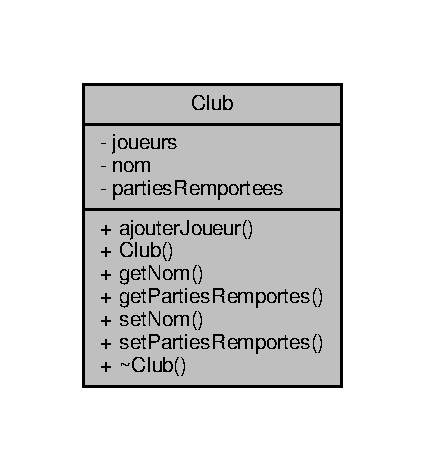
\includegraphics[width=204pt]{class_club__coll__graph}
\end{center}
\end{figure}
\subsubsection*{Fonctions membres publiques}
\begin{DoxyCompactItemize}
\item 
void \hyperlink{class_club_af7cf902fc29f6d587b11a10eec87edff}{ajouter\+Joueur} (char \&lettre, \hyperlink{class_joueur}{Joueur} \&j)
\item 
\hyperlink{class_club_a6d6fa5971608a06394c40453289d6251}{Club} (Q\+String \hyperlink{class_club_a18e1489d02110a82a0c8706f52091002}{nom}=\char`\"{}\char`\"{})
\item 
Q\+String \hyperlink{class_club_aaa3c96659bf305d7a1988ecbd27de30f}{get\+Nom} () const
\item 
int \hyperlink{class_club_af4f28219aa51c3742cddfae4b66cec4b}{get\+Parties\+Remportes} () const
\item 
void \hyperlink{class_club_a6cb8e81d8cfd3d5febd6ce48e33ba94e}{set\+Nom} (Q\+String \&n)
\item 
void \hyperlink{class_club_ad1711f2742e385ef00174b3ebd98b165}{set\+Parties\+Remportes} (int \&p)
\item 
\hyperlink{class_club_a1c2993e141cfa6468284274359cc7de5}{$\sim$\+Club} ()
\end{DoxyCompactItemize}
\subsubsection*{Attributs privés}
\begin{DoxyCompactItemize}
\item 
Q\+Map$<$ char, \hyperlink{class_joueur}{Joueur} $>$ \hyperlink{class_club_a1546f281ba72a07e52cbfd2a60af699b}{joueurs}
\item 
Q\+String \hyperlink{class_club_a18e1489d02110a82a0c8706f52091002}{nom}
\item 
int \hyperlink{class_club_a1c5dd1362656cb4829de483255ffc39a}{parties\+Remportees}
\end{DoxyCompactItemize}


\subsubsection{Description détaillée}


Définition à la ligne \hyperlink{_club_8h_source_l00017}{17} du fichier \hyperlink{_club_8h_source}{Club.\+h}.



\subsubsection{Documentation des constructeurs et destructeur}
\mbox{\Hypertarget{class_club_a6d6fa5971608a06394c40453289d6251}\label{class_club_a6d6fa5971608a06394c40453289d6251}} 
\index{Club@{Club}!Club@{Club}}
\index{Club@{Club}!Club@{Club}}
\paragraph{\texorpdfstring{Club()}{Club()}}
{\footnotesize\ttfamily Club\+::\+Club (\begin{DoxyParamCaption}\item[{Q\+String}]{nom = {\ttfamily \char`\"{}\char`\"{}} }\end{DoxyParamCaption})}



Définition à la ligne \hyperlink{_club_8cpp_source_l00013}{13} du fichier \hyperlink{_club_8cpp_source}{Club.\+cpp}.


\begin{DoxyCode}
00013                       : \hyperlink{class_club_a18e1489d02110a82a0c8706f52091002}{nom}(\hyperlink{class_club_a18e1489d02110a82a0c8706f52091002}{nom}), \hyperlink{class_club_a1c5dd1362656cb4829de483255ffc39a}{partiesRemportees}(0)
00014 \{
00015     qDebug() << Q\_FUNC\_INFO << \hyperlink{class_club_a18e1489d02110a82a0c8706f52091002}{nom} << \textcolor{keyword}{this};
00016 \}
\end{DoxyCode}
\mbox{\Hypertarget{class_club_a1c2993e141cfa6468284274359cc7de5}\label{class_club_a1c2993e141cfa6468284274359cc7de5}} 
\index{Club@{Club}!````~Club@{$\sim$\+Club}}
\index{````~Club@{$\sim$\+Club}!Club@{Club}}
\paragraph{\texorpdfstring{$\sim$\+Club()}{~Club()}}
{\footnotesize\ttfamily Club\+::$\sim$\+Club (\begin{DoxyParamCaption}{ }\end{DoxyParamCaption})}



Définition à la ligne \hyperlink{_club_8cpp_source_l00018}{18} du fichier \hyperlink{_club_8cpp_source}{Club.\+cpp}.


\begin{DoxyCode}
00019 \{
00020     qDebug() << Q\_FUNC\_INFO << \textcolor{keyword}{this};
00021 \}
\end{DoxyCode}


\subsubsection{Documentation des fonctions membres}
\mbox{\Hypertarget{class_club_af7cf902fc29f6d587b11a10eec87edff}\label{class_club_af7cf902fc29f6d587b11a10eec87edff}} 
\index{Club@{Club}!ajouter\+Joueur@{ajouter\+Joueur}}
\index{ajouter\+Joueur@{ajouter\+Joueur}!Club@{Club}}
\paragraph{\texorpdfstring{ajouter\+Joueur()}{ajouterJoueur()}}
{\footnotesize\ttfamily void Club\+::ajouter\+Joueur (\begin{DoxyParamCaption}\item[{char \&}]{lettre,  }\item[{\hyperlink{class_joueur}{Joueur} \&}]{j }\end{DoxyParamCaption})}



Définition à la ligne \hyperlink{_club_8cpp_source_l00043}{43} du fichier \hyperlink{_club_8cpp_source}{Club.\+cpp}.



Références \hyperlink{_club_8h_source_l00022}{joueurs}.


\begin{DoxyCode}
00044 \{
00045     \hyperlink{class_club_a1546f281ba72a07e52cbfd2a60af699b}{joueurs}.insert(lettre,j);
00046 \}
\end{DoxyCode}
\mbox{\Hypertarget{class_club_aaa3c96659bf305d7a1988ecbd27de30f}\label{class_club_aaa3c96659bf305d7a1988ecbd27de30f}} 
\index{Club@{Club}!get\+Nom@{get\+Nom}}
\index{get\+Nom@{get\+Nom}!Club@{Club}}
\paragraph{\texorpdfstring{get\+Nom()}{getNom()}}
{\footnotesize\ttfamily Q\+String Club\+::get\+Nom (\begin{DoxyParamCaption}{ }\end{DoxyParamCaption}) const}



Définition à la ligne \hyperlink{_club_8cpp_source_l00023}{23} du fichier \hyperlink{_club_8cpp_source}{Club.\+cpp}.



Références \hyperlink{_club_8h_source_l00020}{nom}.


\begin{DoxyCode}
00024 \{
00025     \textcolor{keywordflow}{return} this->\hyperlink{class_club_a18e1489d02110a82a0c8706f52091002}{nom};
00026 \}
\end{DoxyCode}
\mbox{\Hypertarget{class_club_af4f28219aa51c3742cddfae4b66cec4b}\label{class_club_af4f28219aa51c3742cddfae4b66cec4b}} 
\index{Club@{Club}!get\+Parties\+Remportes@{get\+Parties\+Remportes}}
\index{get\+Parties\+Remportes@{get\+Parties\+Remportes}!Club@{Club}}
\paragraph{\texorpdfstring{get\+Parties\+Remportes()}{getPartiesRemportes()}}
{\footnotesize\ttfamily int Club\+::get\+Parties\+Remportes (\begin{DoxyParamCaption}{ }\end{DoxyParamCaption}) const}



Définition à la ligne \hyperlink{_club_8cpp_source_l00033}{33} du fichier \hyperlink{_club_8cpp_source}{Club.\+cpp}.



Références \hyperlink{_club_8h_source_l00021}{parties\+Remportees}.


\begin{DoxyCode}
00034 \{
00035     \textcolor{keywordflow}{return} this->\hyperlink{class_club_a1c5dd1362656cb4829de483255ffc39a}{partiesRemportees};
00036 \}
\end{DoxyCode}
\mbox{\Hypertarget{class_club_a6cb8e81d8cfd3d5febd6ce48e33ba94e}\label{class_club_a6cb8e81d8cfd3d5febd6ce48e33ba94e}} 
\index{Club@{Club}!set\+Nom@{set\+Nom}}
\index{set\+Nom@{set\+Nom}!Club@{Club}}
\paragraph{\texorpdfstring{set\+Nom()}{setNom()}}
{\footnotesize\ttfamily void Club\+::set\+Nom (\begin{DoxyParamCaption}\item[{Q\+String \&}]{n }\end{DoxyParamCaption})}



Définition à la ligne \hyperlink{_club_8cpp_source_l00028}{28} du fichier \hyperlink{_club_8cpp_source}{Club.\+cpp}.



Références \hyperlink{_club_8h_source_l00020}{nom}.


\begin{DoxyCode}
00029 \{
00030     \hyperlink{class_club_a18e1489d02110a82a0c8706f52091002}{nom} = n;
00031 \}
\end{DoxyCode}
\mbox{\Hypertarget{class_club_ad1711f2742e385ef00174b3ebd98b165}\label{class_club_ad1711f2742e385ef00174b3ebd98b165}} 
\index{Club@{Club}!set\+Parties\+Remportes@{set\+Parties\+Remportes}}
\index{set\+Parties\+Remportes@{set\+Parties\+Remportes}!Club@{Club}}
\paragraph{\texorpdfstring{set\+Parties\+Remportes()}{setPartiesRemportes()}}
{\footnotesize\ttfamily void Club\+::set\+Parties\+Remportes (\begin{DoxyParamCaption}\item[{int \&}]{p }\end{DoxyParamCaption})}



Définition à la ligne \hyperlink{_club_8cpp_source_l00038}{38} du fichier \hyperlink{_club_8cpp_source}{Club.\+cpp}.



Références \hyperlink{_club_8h_source_l00021}{parties\+Remportees}.


\begin{DoxyCode}
00039 \{
00040     \hyperlink{class_club_a1c5dd1362656cb4829de483255ffc39a}{partiesRemportees} = p;
00041 \}
\end{DoxyCode}


\subsubsection{Documentation des données membres}
\mbox{\Hypertarget{class_club_a1546f281ba72a07e52cbfd2a60af699b}\label{class_club_a1546f281ba72a07e52cbfd2a60af699b}} 
\index{Club@{Club}!joueurs@{joueurs}}
\index{joueurs@{joueurs}!Club@{Club}}
\paragraph{\texorpdfstring{joueurs}{joueurs}}
{\footnotesize\ttfamily Q\+Map$<$char,\hyperlink{class_joueur}{Joueur}$>$ Club\+::joueurs\hspace{0.3cm}{\ttfamily [private]}}



Définition à la ligne \hyperlink{_club_8h_source_l00022}{22} du fichier \hyperlink{_club_8h_source}{Club.\+h}.



Référencé par \hyperlink{_club_8cpp_source_l00043}{ajouter\+Joueur()}.

\mbox{\Hypertarget{class_club_a18e1489d02110a82a0c8706f52091002}\label{class_club_a18e1489d02110a82a0c8706f52091002}} 
\index{Club@{Club}!nom@{nom}}
\index{nom@{nom}!Club@{Club}}
\paragraph{\texorpdfstring{nom}{nom}}
{\footnotesize\ttfamily Q\+String Club\+::nom\hspace{0.3cm}{\ttfamily [private]}}



Définition à la ligne \hyperlink{_club_8h_source_l00020}{20} du fichier \hyperlink{_club_8h_source}{Club.\+h}.



Référencé par \hyperlink{_club_8cpp_source_l00023}{get\+Nom()}, et \hyperlink{_club_8cpp_source_l00028}{set\+Nom()}.

\mbox{\Hypertarget{class_club_a1c5dd1362656cb4829de483255ffc39a}\label{class_club_a1c5dd1362656cb4829de483255ffc39a}} 
\index{Club@{Club}!parties\+Remportees@{parties\+Remportees}}
\index{parties\+Remportees@{parties\+Remportees}!Club@{Club}}
\paragraph{\texorpdfstring{parties\+Remportees}{partiesRemportees}}
{\footnotesize\ttfamily int Club\+::parties\+Remportees\hspace{0.3cm}{\ttfamily [private]}}



Définition à la ligne \hyperlink{_club_8h_source_l00021}{21} du fichier \hyperlink{_club_8h_source}{Club.\+h}.



Référencé par \hyperlink{_club_8cpp_source_l00033}{get\+Parties\+Remportes()}, et \hyperlink{_club_8cpp_source_l00038}{set\+Parties\+Remportes()}.



La documentation de cette classe a été générée à partir des fichiers suivants \+:\begin{DoxyCompactItemize}
\item 
\hyperlink{_club_8h}{Club.\+h}\item 
\hyperlink{_club_8cpp}{Club.\+cpp}\end{DoxyCompactItemize}

\hypertarget{class_communication}{}\subsection{Référence de la classe Communication}
\label{class_communication}\index{Communication@{Communication}}


Déclaration de la classe \hyperlink{class_communication}{Communication}.  




{\ttfamily \#include $<$Communication.\+h$>$}



Graphe de collaboration de Communication\+:
\nopagebreak
\begin{figure}[H]
\begin{center}
\leavevmode
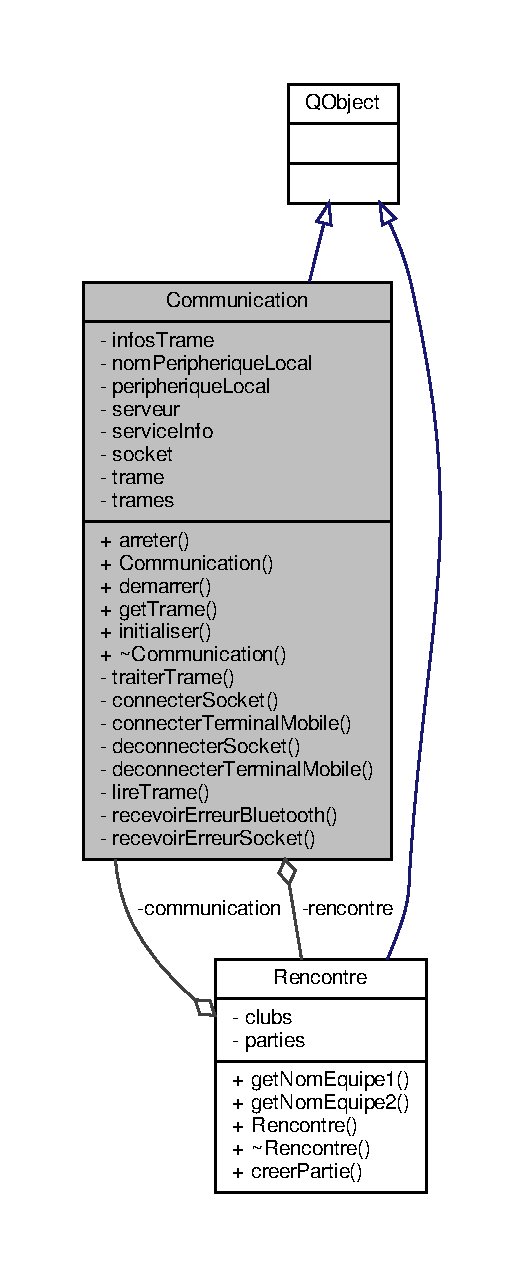
\includegraphics[height=550pt]{class_communication__coll__graph}
\end{center}
\end{figure}
\subsubsection*{Signaux}
\begin{DoxyCompactItemize}
\item 
void \hyperlink{class_communication_af5444d470230a6e817ca8bc9484eb169}{changement\+Etat\+Partie} ()
\item 
void \hyperlink{class_communication_a3d8a1dccee9867e6b84932ddc3072b45}{creation\+Partie} (Q\+String\+List info\+Trame)
\item 
void \hyperlink{class_communication_af3430c844d728e4ec3961744243324e1}{debut\+Rencontre} (Q\+String club1, Q\+String club2)
\item 
void \hyperlink{class_communication_ab2dd9f10ceaba18016017104683b6fc1}{demande\+Temps\+Mort} ()
\item 
void \hyperlink{class_communication_a4c828450e0ff92818c878ee28f240662}{detection\+N\+ET} ()
\item 
void \hyperlink{class_communication_acf4446d47652e0c508296e52df6fb11b}{nouveau\+Score\+Partie} ()
\end{DoxyCompactItemize}
\subsubsection*{Fonctions membres publiques}
\begin{DoxyCompactItemize}
\item 
void \hyperlink{class_communication_a1f4b02441803f9c8e231cb9f304d776b}{arreter} ()
\begin{DoxyCompactList}\small\item\em Méthode qui arrête le serveur Bluetooth. \end{DoxyCompactList}\item 
\hyperlink{class_communication_a56cf4b262e592bcae1d987c3dd00487f}{Communication} (\hyperlink{class_q_object}{Q\+Object} $\ast$parent=nullptr)
\begin{DoxyCompactList}\small\item\em Constructeur de la classe \hyperlink{class_communication}{Communication}. \end{DoxyCompactList}\item 
void \hyperlink{class_communication_af29ea9a1c2ce29436f2331c322f6ebbf}{demarrer} ()
\begin{DoxyCompactList}\small\item\em Méthode qui démarre le serveur Bluetooth. \end{DoxyCompactList}\item 
Q\+String \hyperlink{class_communication_ad8dbd75b168bc02c76306361e650bbba}{get\+Trame} () const
\item 
void \hyperlink{class_communication_a2c10a52807bc7bdc520ec3fae622f672}{initialiser} ()
\begin{DoxyCompactList}\small\item\em Méthode qui prépare la connexion Bluetooth en mode serveur. \end{DoxyCompactList}\item 
\hyperlink{class_communication_a75ba08ce908d45251e28e4c1db94e6f4}{$\sim$\+Communication} ()
\begin{DoxyCompactList}\small\item\em Destructeur de la classe \hyperlink{class_communication}{Communication}. \end{DoxyCompactList}\end{DoxyCompactItemize}
\subsubsection*{Connecteurs privés}
\begin{DoxyCompactItemize}
\item 
void \hyperlink{class_communication_a1ef7e4107d98346290f19f76d7eecf32}{connecter\+Socket} ()
\item 
void \hyperlink{class_communication_a9640339b93f4a99f80426b7345615037}{connecter\+Terminal\+Mobile} (const Q\+Bluetooth\+Address \&adresse)
\item 
void \hyperlink{class_communication_a5280c11bea5ead32e7a7101fd5b0f9b2}{deconnecter\+Socket} ()
\item 
void \hyperlink{class_communication_aeeb47bc3c4d7419fefb737168638442e}{deconnecter\+Terminal\+Mobile} (const Q\+Bluetooth\+Address \&adresse)
\item 
void \hyperlink{class_communication_ad99afe857470e6e95432b3adcb97fea2}{lire\+Trame} ()
\item 
void \hyperlink{class_communication_adbbab5630096d6374c4d7e52508b8a37}{recevoir\+Erreur\+Bluetooth} (Q\+Bluetooth\+Local\+Device\+::\+Error erreur\+Bluetooth)
\item 
void \hyperlink{class_communication_a94a9c34e683d590fc6abbc4111a57f29}{recevoir\+Erreur\+Socket} (Q\+Bluetooth\+Socket\+::\+Socket\+Error e)
\end{DoxyCompactItemize}
\subsubsection*{Fonctions membres privées}
\begin{DoxyCompactItemize}
\item 
bool \hyperlink{class_communication_a1f17fd8330b55b3ab30263d15e6e740b}{traiter\+Trame} (Q\+String\+List \hyperlink{class_communication_a219fe9a4cd04470241f26f1f6159d721}{infos\+Trame})
\end{DoxyCompactItemize}
\subsubsection*{Attributs privés}
\begin{DoxyCompactItemize}
\item 
Q\+String\+List \hyperlink{class_communication_a219fe9a4cd04470241f26f1f6159d721}{infos\+Trame}
\begin{DoxyCompactList}\small\item\em Les informations transmises dans la trame. \end{DoxyCompactList}\item 
Q\+String \hyperlink{class_communication_acfe0b2b569ebf174fcdd766272b89ba8}{nom\+Peripherique\+Local}
\begin{DoxyCompactList}\small\item\em Nom du périphérique local. \end{DoxyCompactList}\item 
Q\+Bluetooth\+Local\+Device \hyperlink{class_communication_a2d643d199169dfe1d258df54d3ee5728}{peripherique\+Local}
\begin{DoxyCompactList}\small\item\em L\textquotesingle{}interface Bluetooth de la Raspberry Pi. \end{DoxyCompactList}\item 
\hyperlink{class_rencontre}{Rencontre} $\ast$ \hyperlink{class_communication_acb471e5da168acc149c5e4e90d8b601c}{rencontre}
\item 
Q\+Bluetooth\+Server $\ast$ \hyperlink{class_communication_a6384747297d6efa9e8fd2fc79ed0c269}{serveur}
\begin{DoxyCompactList}\small\item\em Le serveur Bluetooth. \end{DoxyCompactList}\item 
Q\+Bluetooth\+Service\+Info \hyperlink{class_communication_aa7f9ee5e5d90336a56857ebc229e4274}{service\+Info}
\begin{DoxyCompactList}\small\item\em Informations sur le service bluetooth. \end{DoxyCompactList}\item 
Q\+Bluetooth\+Socket $\ast$ \hyperlink{class_communication_aa4ddc3151b305db0135d5826384645cc}{socket}
\begin{DoxyCompactList}\small\item\em La socket de communication Bluetooth. \end{DoxyCompactList}\item 
Q\+String \hyperlink{class_communication_ac8f5004bfaaf7f538ba5ae93255f772b}{trame}
\begin{DoxyCompactList}\small\item\em Une trame extraite. \end{DoxyCompactList}\item 
Q\+String \hyperlink{class_communication_a89b75dc8f2d3427478660b45c01f4186}{trames}
\begin{DoxyCompactList}\small\item\em Les trames recues. \end{DoxyCompactList}\end{DoxyCompactItemize}


\subsubsection{Description détaillée}
Déclaration de la classe \hyperlink{class_communication}{Communication}. 

Cette classe gère la communication Bluetooth 

Définition à la ligne \hyperlink{_communication_8h_source_l00046}{46} du fichier \hyperlink{_communication_8h_source}{Communication.\+h}.



\subsubsection{Documentation des constructeurs et destructeur}
\mbox{\Hypertarget{class_communication_a56cf4b262e592bcae1d987c3dd00487f}\label{class_communication_a56cf4b262e592bcae1d987c3dd00487f}} 
\index{Communication@{Communication}!Communication@{Communication}}
\index{Communication@{Communication}!Communication@{Communication}}
\paragraph{\texorpdfstring{Communication()}{Communication()}}
{\footnotesize\ttfamily Communication\+::\+Communication (\begin{DoxyParamCaption}\item[{\hyperlink{class_q_object}{Q\+Object} $\ast$}]{parent = {\ttfamily nullptr} }\end{DoxyParamCaption})}



Constructeur de la classe \hyperlink{class_communication}{Communication}. 


\begin{DoxyParams}{Paramètres}
{\em parent} & L\textquotesingle{}adresse de l\textquotesingle{}objet parent \\
\hline
\end{DoxyParams}


Définition à la ligne \hyperlink{_communication_8cpp_source_l00020}{20} du fichier \hyperlink{_communication_8cpp_source}{Communication.\+cpp}.



Références \hyperlink{_communication_8cpp_source_l00044}{initialiser()}.


\begin{DoxyCode}
00020                                             : \hyperlink{class_q_object}{QObject}(parent), \hyperlink{class_communication_a6384747297d6efa9e8fd2fc79ed0c269}{serveur}(\textcolor{keyword}{nullptr}), 
      \hyperlink{class_communication_aa4ddc3151b305db0135d5826384645cc}{socket}(\textcolor{keyword}{nullptr})
00021 \{
00022     qDebug() << Q\_FUNC\_INFO;
00023 
00024     \hyperlink{class_communication_a2c10a52807bc7bdc520ec3fae622f672}{initialiser}();
00025 \}
\end{DoxyCode}
\mbox{\Hypertarget{class_communication_a75ba08ce908d45251e28e4c1db94e6f4}\label{class_communication_a75ba08ce908d45251e28e4c1db94e6f4}} 
\index{Communication@{Communication}!````~Communication@{$\sim$\+Communication}}
\index{````~Communication@{$\sim$\+Communication}!Communication@{Communication}}
\paragraph{\texorpdfstring{$\sim$\+Communication()}{~Communication()}}
{\footnotesize\ttfamily Communication\+::$\sim$\+Communication (\begin{DoxyParamCaption}{ }\end{DoxyParamCaption})}



Destructeur de la classe \hyperlink{class_communication}{Communication}. 



Définition à la ligne \hyperlink{_communication_8cpp_source_l00032}{32} du fichier \hyperlink{_communication_8cpp_source}{Communication.\+cpp}.



Références \hyperlink{_communication_8cpp_source_l00099}{arreter()}.


\begin{DoxyCode}
00033 \{
00034     qDebug() << Q\_FUNC\_INFO;
00035 
00036     \hyperlink{class_communication_a1f4b02441803f9c8e231cb9f304d776b}{arreter}();
00037 \}
\end{DoxyCode}


\subsubsection{Documentation des fonctions membres}
\mbox{\Hypertarget{class_communication_a1f4b02441803f9c8e231cb9f304d776b}\label{class_communication_a1f4b02441803f9c8e231cb9f304d776b}} 
\index{Communication@{Communication}!arreter@{arreter}}
\index{arreter@{arreter}!Communication@{Communication}}
\paragraph{\texorpdfstring{arreter()}{arreter()}}
{\footnotesize\ttfamily void Communication\+::arreter (\begin{DoxyParamCaption}{ }\end{DoxyParamCaption})}



Méthode qui arrête le serveur Bluetooth. 

Arrête la communication Bluetooth en mode serveur. 

Définition à la ligne \hyperlink{_communication_8cpp_source_l00099}{99} du fichier \hyperlink{_communication_8cpp_source}{Communication.\+cpp}.



Références \hyperlink{_communication_8cpp_source_l00133}{deconnecter\+Socket()}, \hyperlink{_communication_8h_source_l00053}{peripherique\+Local}, \hyperlink{_communication_8h_source_l00051}{serveur}, et \hyperlink{_communication_8h_source_l00052}{socket}.



Référencé par \hyperlink{_communication_8cpp_source_l00032}{$\sim$\+Communication()}.


\begin{DoxyCode}
00100 \{    
00101     \textcolor{keywordflow}{if} (\hyperlink{class_communication_a6384747297d6efa9e8fd2fc79ed0c269}{serveur} == \textcolor{keyword}{nullptr})
00102         \textcolor{keywordflow}{return};
00103 
00104     \textcolor{keywordflow}{if} (\hyperlink{class_communication_aa4ddc3151b305db0135d5826384645cc}{socket} != \textcolor{keyword}{nullptr})
00105     \{
00106         \hyperlink{class_communication_a5280c11bea5ead32e7a7101fd5b0f9b2}{deconnecterSocket}();
00107     \}
00108 
00109     \textcolor{keyword}{delete} \hyperlink{class_communication_a6384747297d6efa9e8fd2fc79ed0c269}{serveur};
00110     \hyperlink{class_communication_a6384747297d6efa9e8fd2fc79ed0c269}{serveur} = \textcolor{keyword}{nullptr};
00111     qDebug() << Q\_FUNC\_INFO;
00112 
00113     \hyperlink{class_communication_a2d643d199169dfe1d258df54d3ee5728}{peripheriqueLocal}.setHostMode(QBluetoothLocalDevice::HostPoweredOff);
00114 \}
\end{DoxyCode}
\mbox{\Hypertarget{class_communication_af5444d470230a6e817ca8bc9484eb169}\label{class_communication_af5444d470230a6e817ca8bc9484eb169}} 
\index{Communication@{Communication}!changement\+Etat\+Partie@{changement\+Etat\+Partie}}
\index{changement\+Etat\+Partie@{changement\+Etat\+Partie}!Communication@{Communication}}
\paragraph{\texorpdfstring{changement\+Etat\+Partie}{changementEtatPartie}}
{\footnotesize\ttfamily void Communication\+::changement\+Etat\+Partie (\begin{DoxyParamCaption}{ }\end{DoxyParamCaption})\hspace{0.3cm}{\ttfamily [signal]}}



Référencé par \hyperlink{_communication_8cpp_source_l00208}{traiter\+Trame()}.

\mbox{\Hypertarget{class_communication_a1ef7e4107d98346290f19f76d7eecf32}\label{class_communication_a1ef7e4107d98346290f19f76d7eecf32}} 
\index{Communication@{Communication}!connecter\+Socket@{connecter\+Socket}}
\index{connecter\+Socket@{connecter\+Socket}!Communication@{Communication}}
\paragraph{\texorpdfstring{connecter\+Socket}{connecterSocket}}
{\footnotesize\ttfamily void Communication\+::connecter\+Socket (\begin{DoxyParamCaption}{ }\end{DoxyParamCaption})\hspace{0.3cm}{\ttfamily [private]}, {\ttfamily [slot]}}

\begin{DoxyRefDesc}{A faire}
\item[\hyperlink{todo__todo000001}{A faire}]Signaler la connexion de la socket \end{DoxyRefDesc}


Définition à la ligne \hyperlink{_communication_8cpp_source_l00116}{116} du fichier \hyperlink{_communication_8cpp_source}{Communication.\+cpp}.



Références \hyperlink{_communication_8cpp_source_l00133}{deconnecter\+Socket()}, \hyperlink{_communication_8cpp_source_l00173}{lire\+Trame()}, \hyperlink{_communication_8cpp_source_l00142}{recevoir\+Erreur\+Socket()}, \hyperlink{_communication_8h_source_l00051}{serveur}, et \hyperlink{_communication_8h_source_l00052}{socket}.



Référencé par \hyperlink{_communication_8cpp_source_l00073}{demarrer()}.


\begin{DoxyCode}
00117 \{
00118     \hyperlink{class_communication_aa4ddc3151b305db0135d5826384645cc}{socket} = \hyperlink{class_communication_a6384747297d6efa9e8fd2fc79ed0c269}{serveur}->nextPendingConnection();
00119     \textcolor{keywordflow}{if} (!\hyperlink{class_communication_aa4ddc3151b305db0135d5826384645cc}{socket})
00120         \textcolor{keywordflow}{return};
00121 
00122     qDebug() << Q\_FUNC\_INFO;
00123     \hyperlink{class_communication_aa4ddc3151b305db0135d5826384645cc}{socket}->open(QIODevice::ReadOnly);
00124     connect(\hyperlink{class_communication_aa4ddc3151b305db0135d5826384645cc}{socket}, SIGNAL(readyRead()), \textcolor{keyword}{this}, SLOT(\hyperlink{class_communication_ad99afe857470e6e95432b3adcb97fea2}{lireTrame}()));
00125     connect(\hyperlink{class_communication_aa4ddc3151b305db0135d5826384645cc}{socket}, SIGNAL(disconnected()), \textcolor{keyword}{this}, SLOT(\hyperlink{class_communication_a5280c11bea5ead32e7a7101fd5b0f9b2}{deconnecterSocket}()));
00126     connect(\hyperlink{class_communication_aa4ddc3151b305db0135d5826384645cc}{socket}, SIGNAL(error(QBluetoothSocket::SocketError)), \textcolor{keyword}{this}, SLOT(
      \hyperlink{class_communication_a94a9c34e683d590fc6abbc4111a57f29}{recevoirErreurSocket}(QBluetoothSocket::SocketError)));
00127 
00131 \}
\end{DoxyCode}
\mbox{\Hypertarget{class_communication_a9640339b93f4a99f80426b7345615037}\label{class_communication_a9640339b93f4a99f80426b7345615037}} 
\index{Communication@{Communication}!connecter\+Terminal\+Mobile@{connecter\+Terminal\+Mobile}}
\index{connecter\+Terminal\+Mobile@{connecter\+Terminal\+Mobile}!Communication@{Communication}}
\paragraph{\texorpdfstring{connecter\+Terminal\+Mobile}{connecterTerminalMobile}}
{\footnotesize\ttfamily void Communication\+::connecter\+Terminal\+Mobile (\begin{DoxyParamCaption}\item[{const Q\+Bluetooth\+Address \&}]{adresse }\end{DoxyParamCaption})\hspace{0.3cm}{\ttfamily [private]}, {\ttfamily [slot]}}

\begin{DoxyRefDesc}{A faire}
\item[\hyperlink{todo__todo000002}{A faire}]Signaler la connexion d\textquotesingle{}un appareil \end{DoxyRefDesc}


Définition à la ligne \hyperlink{_communication_8cpp_source_l00147}{147} du fichier \hyperlink{_communication_8cpp_source}{Communication.\+cpp}.



Références \hyperlink{_communication_8h_source_l00053}{peripherique\+Local}.



Référencé par \hyperlink{_communication_8cpp_source_l00044}{initialiser()}.


\begin{DoxyCode}
00148 \{
00149     \textcolor{keywordflow}{if} (\hyperlink{class_communication_a2d643d199169dfe1d258df54d3ee5728}{peripheriqueLocal}.pairingStatus(adresse) == QBluetoothLocalDevice::Paired || 
      \hyperlink{class_communication_a2d643d199169dfe1d258df54d3ee5728}{peripheriqueLocal}.pairingStatus(adresse) == QBluetoothLocalDevice::AuthorizedPaired)
00150     \{
00151         qDebug() << Q\_FUNC\_INFO << adresse.toString() << \textcolor{stringliteral}{"appairé"};
00155     \}
00156     \textcolor{keywordflow}{else}
00157         qDebug() << Q\_FUNC\_INFO << adresse.toString() << \textcolor{stringliteral}{"non appairé"};
00158 \}
\end{DoxyCode}
\mbox{\Hypertarget{class_communication_a3d8a1dccee9867e6b84932ddc3072b45}\label{class_communication_a3d8a1dccee9867e6b84932ddc3072b45}} 
\index{Communication@{Communication}!creation\+Partie@{creation\+Partie}}
\index{creation\+Partie@{creation\+Partie}!Communication@{Communication}}
\paragraph{\texorpdfstring{creation\+Partie}{creationPartie}}
{\footnotesize\ttfamily void Communication\+::creation\+Partie (\begin{DoxyParamCaption}\item[{Q\+String\+List}]{info\+Trame }\end{DoxyParamCaption})\hspace{0.3cm}{\ttfamily [signal]}}



Référencé par \hyperlink{_communication_8cpp_source_l00208}{traiter\+Trame()}.

\mbox{\Hypertarget{class_communication_af3430c844d728e4ec3961744243324e1}\label{class_communication_af3430c844d728e4ec3961744243324e1}} 
\index{Communication@{Communication}!debut\+Rencontre@{debut\+Rencontre}}
\index{debut\+Rencontre@{debut\+Rencontre}!Communication@{Communication}}
\paragraph{\texorpdfstring{debut\+Rencontre}{debutRencontre}}
{\footnotesize\ttfamily void Communication\+::debut\+Rencontre (\begin{DoxyParamCaption}\item[{Q\+String}]{club1,  }\item[{Q\+String}]{club2 }\end{DoxyParamCaption})\hspace{0.3cm}{\ttfamily [signal]}}



Référencé par \hyperlink{_communication_8cpp_source_l00208}{traiter\+Trame()}.

\mbox{\Hypertarget{class_communication_a5280c11bea5ead32e7a7101fd5b0f9b2}\label{class_communication_a5280c11bea5ead32e7a7101fd5b0f9b2}} 
\index{Communication@{Communication}!deconnecter\+Socket@{deconnecter\+Socket}}
\index{deconnecter\+Socket@{deconnecter\+Socket}!Communication@{Communication}}
\paragraph{\texorpdfstring{deconnecter\+Socket}{deconnecterSocket}}
{\footnotesize\ttfamily void Communication\+::deconnecter\+Socket (\begin{DoxyParamCaption}{ }\end{DoxyParamCaption})\hspace{0.3cm}{\ttfamily [private]}, {\ttfamily [slot]}}



Définition à la ligne \hyperlink{_communication_8cpp_source_l00133}{133} du fichier \hyperlink{_communication_8cpp_source}{Communication.\+cpp}.



Références \hyperlink{_communication_8h_source_l00052}{socket}.



Référencé par \hyperlink{_communication_8cpp_source_l00099}{arreter()}, et \hyperlink{_communication_8cpp_source_l00116}{connecter\+Socket()}.


\begin{DoxyCode}
00134 \{    
00135     \textcolor{keywordflow}{if} (\hyperlink{class_communication_aa4ddc3151b305db0135d5826384645cc}{socket}->isOpen())
00136        \hyperlink{class_communication_aa4ddc3151b305db0135d5826384645cc}{socket}->close();
00137     \textcolor{keyword}{delete} \hyperlink{class_communication_aa4ddc3151b305db0135d5826384645cc}{socket};
00138     \hyperlink{class_communication_aa4ddc3151b305db0135d5826384645cc}{socket} = \textcolor{keyword}{nullptr};
00139     qDebug() << Q\_FUNC\_INFO;
00140 \}
\end{DoxyCode}
\mbox{\Hypertarget{class_communication_aeeb47bc3c4d7419fefb737168638442e}\label{class_communication_aeeb47bc3c4d7419fefb737168638442e}} 
\index{Communication@{Communication}!deconnecter\+Terminal\+Mobile@{deconnecter\+Terminal\+Mobile}}
\index{deconnecter\+Terminal\+Mobile@{deconnecter\+Terminal\+Mobile}!Communication@{Communication}}
\paragraph{\texorpdfstring{deconnecter\+Terminal\+Mobile}{deconnecterTerminalMobile}}
{\footnotesize\ttfamily void Communication\+::deconnecter\+Terminal\+Mobile (\begin{DoxyParamCaption}\item[{const Q\+Bluetooth\+Address \&}]{adresse }\end{DoxyParamCaption})\hspace{0.3cm}{\ttfamily [private]}, {\ttfamily [slot]}}

\begin{DoxyRefDesc}{A faire}
\item[\hyperlink{todo__todo000003}{A faire}]Signaler la déconnexion d\textquotesingle{}un appareil \end{DoxyRefDesc}


Définition à la ligne \hyperlink{_communication_8cpp_source_l00160}{160} du fichier \hyperlink{_communication_8cpp_source}{Communication.\+cpp}.



Référencé par \hyperlink{_communication_8cpp_source_l00044}{initialiser()}.


\begin{DoxyCode}
00161 \{
00162     qDebug() << Q\_FUNC\_INFO << adresse;
00166 \}
\end{DoxyCode}
\mbox{\Hypertarget{class_communication_ab2dd9f10ceaba18016017104683b6fc1}\label{class_communication_ab2dd9f10ceaba18016017104683b6fc1}} 
\index{Communication@{Communication}!demande\+Temps\+Mort@{demande\+Temps\+Mort}}
\index{demande\+Temps\+Mort@{demande\+Temps\+Mort}!Communication@{Communication}}
\paragraph{\texorpdfstring{demande\+Temps\+Mort}{demandeTempsMort}}
{\footnotesize\ttfamily void Communication\+::demande\+Temps\+Mort (\begin{DoxyParamCaption}{ }\end{DoxyParamCaption})\hspace{0.3cm}{\ttfamily [signal]}}



Référencé par \hyperlink{_communication_8cpp_source_l00208}{traiter\+Trame()}.

\mbox{\Hypertarget{class_communication_af29ea9a1c2ce29436f2331c322f6ebbf}\label{class_communication_af29ea9a1c2ce29436f2331c322f6ebbf}} 
\index{Communication@{Communication}!demarrer@{demarrer}}
\index{demarrer@{demarrer}!Communication@{Communication}}
\paragraph{\texorpdfstring{demarrer()}{demarrer()}}
{\footnotesize\ttfamily void Communication\+::demarrer (\begin{DoxyParamCaption}{ }\end{DoxyParamCaption})}



Méthode qui démarre le serveur Bluetooth. 

Démarre la communication Bluetooth en mode serveur. 

Définition à la ligne \hyperlink{_communication_8cpp_source_l00073}{73} du fichier \hyperlink{_communication_8cpp_source}{Communication.\+cpp}.



Références \hyperlink{_communication_8cpp_source_l00116}{connecter\+Socket()}, \hyperlink{_communication_8h_afd6061bebcd621de34bc921326538181}{nom\+Service()}, \hyperlink{_communication_8h_source_l00053}{peripherique\+Local}, \hyperlink{_communication_8h_source_l00051}{serveur}, \hyperlink{_communication_8h_source_l00054}{service\+Info}, et \hyperlink{_communication_8h_a6f285f3a7cee5c6573729d7e6b99dbf4}{uuid\+Service()}.



Référencé par \hyperlink{_i_h_m_afficheur_8cpp_source_l00074}{I\+H\+M\+Afficheur\+::initialiser\+Communication()}.


\begin{DoxyCode}
00074 \{
00075     \textcolor{comment}{// vérifier la présence du Bluetooth}
00076     \textcolor{keywordflow}{if} (\hyperlink{class_communication_a2d643d199169dfe1d258df54d3ee5728}{peripheriqueLocal}.isValid() && \hyperlink{class_communication_a6384747297d6efa9e8fd2fc79ed0c269}{serveur} == \textcolor{keyword}{nullptr})
00077     \{
00078         \textcolor{comment}{// créer une socket serveur}
00079         \hyperlink{class_communication_a6384747297d6efa9e8fd2fc79ed0c269}{serveur} = \textcolor{keyword}{new} QBluetoothServer(QBluetoothServiceInfo::RfcommProtocol, \textcolor{keyword}{this});
00080 
00081         \textcolor{comment}{// connecter les signaux et les slots}
00082         connect(\hyperlink{class_communication_a6384747297d6efa9e8fd2fc79ed0c269}{serveur}, SIGNAL(newConnection()), \textcolor{keyword}{this}, SLOT(
      \hyperlink{class_communication_a1ef7e4107d98346290f19f76d7eecf32}{connecterSocket}()));
00083 
00084         \textcolor{comment}{// placer le serveur en écoute}
00085         QBluetoothUuid uuid = QBluetoothUuid(\hyperlink{_communication_8h_a6f285f3a7cee5c6573729d7e6b99dbf4}{uuidService});
00086         \hyperlink{class_communication_aa7f9ee5e5d90336a56857ebc229e4274}{serviceInfo} = \hyperlink{class_communication_a6384747297d6efa9e8fd2fc79ed0c269}{serveur}->listen(uuid, \hyperlink{_communication_8h_afd6061bebcd621de34bc921326538181}{nomService});
00087 
00088         qDebug() << Q\_FUNC\_INFO << \textcolor{stringliteral}{"Attente de connexion"};
00089     \}
00090     \textcolor{keywordflow}{else}
00091         qDebug() << Q\_FUNC\_INFO << \textcolor{stringliteral}{"Bluetooth non disponible !"};
00092 \}
\end{DoxyCode}
\mbox{\Hypertarget{class_communication_a4c828450e0ff92818c878ee28f240662}\label{class_communication_a4c828450e0ff92818c878ee28f240662}} 
\index{Communication@{Communication}!detection\+N\+ET@{detection\+N\+ET}}
\index{detection\+N\+ET@{detection\+N\+ET}!Communication@{Communication}}
\paragraph{\texorpdfstring{detection\+N\+ET}{detectionNET}}
{\footnotesize\ttfamily void Communication\+::detection\+N\+ET (\begin{DoxyParamCaption}{ }\end{DoxyParamCaption})\hspace{0.3cm}{\ttfamily [signal]}}



Référencé par \hyperlink{_communication_8cpp_source_l00208}{traiter\+Trame()}.

\mbox{\Hypertarget{class_communication_ad8dbd75b168bc02c76306361e650bbba}\label{class_communication_ad8dbd75b168bc02c76306361e650bbba}} 
\index{Communication@{Communication}!get\+Trame@{get\+Trame}}
\index{get\+Trame@{get\+Trame}!Communication@{Communication}}
\paragraph{\texorpdfstring{get\+Trame()}{getTrame()}}
{\footnotesize\ttfamily Q\+String Communication\+::get\+Trame (\begin{DoxyParamCaption}{ }\end{DoxyParamCaption}) const}



Définition à la ligne \hyperlink{_communication_8cpp_source_l00252}{252} du fichier \hyperlink{_communication_8cpp_source}{Communication.\+cpp}.



Références \hyperlink{_communication_8h_source_l00056}{trame}.


\begin{DoxyCode}
00253 \{
00254     \textcolor{keywordflow}{return} \hyperlink{class_communication_ac8f5004bfaaf7f538ba5ae93255f772b}{trame};
00255 \}
\end{DoxyCode}
\mbox{\Hypertarget{class_communication_a2c10a52807bc7bdc520ec3fae622f672}\label{class_communication_a2c10a52807bc7bdc520ec3fae622f672}} 
\index{Communication@{Communication}!initialiser@{initialiser}}
\index{initialiser@{initialiser}!Communication@{Communication}}
\paragraph{\texorpdfstring{initialiser()}{initialiser()}}
{\footnotesize\ttfamily void Communication\+::initialiser (\begin{DoxyParamCaption}{ }\end{DoxyParamCaption})}



Méthode qui prépare la connexion Bluetooth en mode serveur. 

Initialise la liaison Bluetooth en mode serveur. 

Définition à la ligne \hyperlink{_communication_8cpp_source_l00044}{44} du fichier \hyperlink{_communication_8cpp_source}{Communication.\+cpp}.



Références \hyperlink{_communication_8cpp_source_l00147}{connecter\+Terminal\+Mobile()}, \hyperlink{_communication_8cpp_source_l00160}{deconnecter\+Terminal\+Mobile()}, \hyperlink{_communication_8h_source_l00055}{nom\+Peripherique\+Local}, \hyperlink{_communication_8h_source_l00053}{peripherique\+Local}, et \hyperlink{_communication_8cpp_source_l00168}{recevoir\+Erreur\+Bluetooth()}.



Référencé par \hyperlink{_communication_8cpp_source_l00020}{Communication()}.


\begin{DoxyCode}
00045 \{
00046     \textcolor{comment}{// vérifier la présence du Bluetooth}
00047     \textcolor{keywordflow}{if} (\hyperlink{class_communication_a2d643d199169dfe1d258df54d3ee5728}{peripheriqueLocal}.isValid())
00048     \{
00049         \textcolor{comment}{// activer le bluetooth}
00050         \hyperlink{class_communication_a2d643d199169dfe1d258df54d3ee5728}{peripheriqueLocal}.powerOn();
00051 
00052         \textcolor{comment}{// récupérer le nom du périphérique local}
00053         \hyperlink{class_communication_acfe0b2b569ebf174fcdd766272b89ba8}{nomPeripheriqueLocal} = \hyperlink{class_communication_a2d643d199169dfe1d258df54d3ee5728}{peripheriqueLocal}.name();
00054         qDebug() << Q\_FUNC\_INFO << \hyperlink{class_communication_acfe0b2b569ebf174fcdd766272b89ba8}{nomPeripheriqueLocal};
00055 
00056         \textcolor{comment}{// rendre le périphérique local découvrable et jumelable}
00057         \hyperlink{class_communication_a2d643d199169dfe1d258df54d3ee5728}{peripheriqueLocal}.setHostMode(QBluetoothLocalDevice::HostDiscoverable);
00058 
00059         \textcolor{comment}{// connecter les signaux et les slots}
00060         connect(&\hyperlink{class_communication_a2d643d199169dfe1d258df54d3ee5728}{peripheriqueLocal}, SIGNAL(deviceConnected(QBluetoothAddress)), \textcolor{keyword}{this}, SLOT
      (\hyperlink{class_communication_a9640339b93f4a99f80426b7345615037}{connecterTerminalMobile}(QBluetoothAddress)));
00061         connect(&\hyperlink{class_communication_a2d643d199169dfe1d258df54d3ee5728}{peripheriqueLocal}, SIGNAL(deviceDisconnected(QBluetoothAddress)), \textcolor{keyword}{this}, 
      SLOT(\hyperlink{class_communication_aeeb47bc3c4d7419fefb737168638442e}{deconnecterTerminalMobile}(QBluetoothAddress)));
00062         connect(&\hyperlink{class_communication_a2d643d199169dfe1d258df54d3ee5728}{peripheriqueLocal}, SIGNAL(error(QBluetoothLocalDevice::Error)), \textcolor{keyword}{this}, 
      SLOT(\hyperlink{class_communication_adbbab5630096d6374c4d7e52508b8a37}{recevoirErreurBluetooth}(QBluetoothLocalDevice::Error)));
00063     \}
00064     \textcolor{keywordflow}{else}
00065         qDebug() << Q\_FUNC\_INFO << \textcolor{stringliteral}{"Bluetooth non disponible !"};
00066 \}
\end{DoxyCode}
\mbox{\Hypertarget{class_communication_ad99afe857470e6e95432b3adcb97fea2}\label{class_communication_ad99afe857470e6e95432b3adcb97fea2}} 
\index{Communication@{Communication}!lire\+Trame@{lire\+Trame}}
\index{lire\+Trame@{lire\+Trame}!Communication@{Communication}}
\paragraph{\texorpdfstring{lire\+Trame}{lireTrame}}
{\footnotesize\ttfamily void Communication\+::lire\+Trame (\begin{DoxyParamCaption}{ }\end{DoxyParamCaption})\hspace{0.3cm}{\ttfamily [private]}, {\ttfamily [slot]}}



Définition à la ligne \hyperlink{_communication_8cpp_source_l00173}{173} du fichier \hyperlink{_communication_8cpp_source}{Communication.\+cpp}.



Références \hyperlink{_communication_8h_source_l00019}{E\+N\+T\+E\+T\+E\+\_\+\+T\+R\+A\+ME}, \hyperlink{_communication_8h_source_l00058}{infos\+Trame}, \hyperlink{_communication_8h_source_l00052}{socket}, \hyperlink{_communication_8cpp_source_l00208}{traiter\+Trame()}, \hyperlink{_communication_8h_source_l00056}{trame}, et \hyperlink{_communication_8h_source_l00057}{trames}.



Référencé par \hyperlink{_communication_8cpp_source_l00116}{connecter\+Socket()}.


\begin{DoxyCode}
00174 \{
00175     QByteArray donnees;
00176 
00177     \textcolor{comment}{// lit les données reçues}
00178     donnees = \hyperlink{class_communication_aa4ddc3151b305db0135d5826384645cc}{socket}->readAll();
00179     qDebug() << Q\_FUNC\_INFO << donnees;
00180 
00181     \textcolor{comment}{// ajoute les données reçues}
00182     \hyperlink{class_communication_ac8f5004bfaaf7f538ba5ae93255f772b}{trame} += QString(donnees.data());
00183     qDebug() << Q\_FUNC\_INFO << \hyperlink{class_communication_ac8f5004bfaaf7f538ba5ae93255f772b}{trame};
00184 
00185     \textcolor{comment}{// au moins une trame complète reçue ?}
00186     \textcolor{keywordflow}{if}(trame.startsWith(\hyperlink{_communication_8h_a226742d7ade287673fb2295df90f462b}{ENTETE\_TRAME}) && trame.endsWith(\textcolor{stringliteral}{"\(\backslash\)r\(\backslash\)n"}))
00187     \{
00188         \textcolor{comment}{// si plusieurs trames reçues}
00189         QStringList \hyperlink{class_communication_a89b75dc8f2d3427478660b45c01f4186}{trames} = trame.split(\textcolor{stringliteral}{"\(\backslash\)r\(\backslash\)n"}, QString::SkipEmptyParts);
00190         qDebug() << Q\_FUNC\_INFO << \hyperlink{class_communication_a89b75dc8f2d3427478660b45c01f4186}{trames};
00191 
00192         \textcolor{comment}{// traite les trames reçues}
00193         \textcolor{keywordflow}{for}(\textcolor{keywordtype}{int} i = 0; i < trames.count(); ++i)
00194         \{
00195             qDebug() << Q\_FUNC\_INFO << i << trames[i];
00196 
00197             \textcolor{comment}{// découpe les champs de la trame}
00198             \hyperlink{class_communication_a219fe9a4cd04470241f26f1f6159d721}{infosTrame} = trames[i].split(\textcolor{stringliteral}{";"});
00199 
00200             \hyperlink{class_communication_a1f17fd8330b55b3ab30263d15e6e740b}{traiterTrame}(\hyperlink{class_communication_a219fe9a4cd04470241f26f1f6159d721}{infosTrame});
00201         \}
00202 
00203         \textcolor{comment}{// reinitialise trame pour la prochaine réception}
00204         trame.clear();
00205     \}
00206 \}
\end{DoxyCode}
\mbox{\Hypertarget{class_communication_acf4446d47652e0c508296e52df6fb11b}\label{class_communication_acf4446d47652e0c508296e52df6fb11b}} 
\index{Communication@{Communication}!nouveau\+Score\+Partie@{nouveau\+Score\+Partie}}
\index{nouveau\+Score\+Partie@{nouveau\+Score\+Partie}!Communication@{Communication}}
\paragraph{\texorpdfstring{nouveau\+Score\+Partie}{nouveauScorePartie}}
{\footnotesize\ttfamily void Communication\+::nouveau\+Score\+Partie (\begin{DoxyParamCaption}{ }\end{DoxyParamCaption})\hspace{0.3cm}{\ttfamily [signal]}}



Référencé par \hyperlink{_communication_8cpp_source_l00208}{traiter\+Trame()}.

\mbox{\Hypertarget{class_communication_adbbab5630096d6374c4d7e52508b8a37}\label{class_communication_adbbab5630096d6374c4d7e52508b8a37}} 
\index{Communication@{Communication}!recevoir\+Erreur\+Bluetooth@{recevoir\+Erreur\+Bluetooth}}
\index{recevoir\+Erreur\+Bluetooth@{recevoir\+Erreur\+Bluetooth}!Communication@{Communication}}
\paragraph{\texorpdfstring{recevoir\+Erreur\+Bluetooth}{recevoirErreurBluetooth}}
{\footnotesize\ttfamily void Communication\+::recevoir\+Erreur\+Bluetooth (\begin{DoxyParamCaption}\item[{Q\+Bluetooth\+Local\+Device\+::\+Error}]{erreur\+Bluetooth }\end{DoxyParamCaption})\hspace{0.3cm}{\ttfamily [private]}, {\ttfamily [slot]}}



Définition à la ligne \hyperlink{_communication_8cpp_source_l00168}{168} du fichier \hyperlink{_communication_8cpp_source}{Communication.\+cpp}.



Référencé par \hyperlink{_communication_8cpp_source_l00044}{initialiser()}.


\begin{DoxyCode}
00169 \{
00170     qDebug() << Q\_FUNC\_INFO << erreurBluetooth;
00171 \}
\end{DoxyCode}
\mbox{\Hypertarget{class_communication_a94a9c34e683d590fc6abbc4111a57f29}\label{class_communication_a94a9c34e683d590fc6abbc4111a57f29}} 
\index{Communication@{Communication}!recevoir\+Erreur\+Socket@{recevoir\+Erreur\+Socket}}
\index{recevoir\+Erreur\+Socket@{recevoir\+Erreur\+Socket}!Communication@{Communication}}
\paragraph{\texorpdfstring{recevoir\+Erreur\+Socket}{recevoirErreurSocket}}
{\footnotesize\ttfamily void Communication\+::recevoir\+Erreur\+Socket (\begin{DoxyParamCaption}\item[{Q\+Bluetooth\+Socket\+::\+Socket\+Error}]{e }\end{DoxyParamCaption})\hspace{0.3cm}{\ttfamily [private]}, {\ttfamily [slot]}}



Définition à la ligne \hyperlink{_communication_8cpp_source_l00142}{142} du fichier \hyperlink{_communication_8cpp_source}{Communication.\+cpp}.



Référencé par \hyperlink{_communication_8cpp_source_l00116}{connecter\+Socket()}.


\begin{DoxyCode}
00143 \{
00144     qDebug() << Q\_FUNC\_INFO << e;
00145 \}
\end{DoxyCode}
\mbox{\Hypertarget{class_communication_a1f17fd8330b55b3ab30263d15e6e740b}\label{class_communication_a1f17fd8330b55b3ab30263d15e6e740b}} 
\index{Communication@{Communication}!traiter\+Trame@{traiter\+Trame}}
\index{traiter\+Trame@{traiter\+Trame}!Communication@{Communication}}
\paragraph{\texorpdfstring{traiter\+Trame()}{traiterTrame()}}
{\footnotesize\ttfamily bool Communication\+::traiter\+Trame (\begin{DoxyParamCaption}\item[{Q\+String\+List}]{infos\+Trame }\end{DoxyParamCaption})\hspace{0.3cm}{\ttfamily [private]}}

\begin{DoxyRefDesc}{A faire}
\item[\hyperlink{todo__todo000004}{A faire}]Définir les constantes pour les champs de la trame !!! \end{DoxyRefDesc}


Définition à la ligne \hyperlink{_communication_8cpp_source_l00208}{208} du fichier \hyperlink{_communication_8cpp_source}{Communication.\+cpp}.



Références \hyperlink{_communication_8h_source_l00020}{C\+H\+A\+M\+P\+\_\+\+T\+Y\+P\+E\+\_\+\+T\+R\+A\+ME}, \hyperlink{class_communication_af5444d470230a6e817ca8bc9484eb169}{changement\+Etat\+Partie()}, \hyperlink{class_communication_a3d8a1dccee9867e6b84932ddc3072b45}{creation\+Partie()}, \hyperlink{class_communication_af3430c844d728e4ec3961744243324e1}{debut\+Rencontre()}, \hyperlink{class_communication_ab2dd9f10ceaba18016017104683b6fc1}{demande\+Temps\+Mort()}, \hyperlink{class_communication_a4c828450e0ff92818c878ee28f240662}{detection\+N\+E\+T()}, \hyperlink{_communication_8h_source_l00031}{E\+T\+A\+T\+\_\+\+P\+A\+R\+T\+IE}, \hyperlink{_communication_8h_source_l00029}{I\+N\+F\+O\+\_\+\+P\+A\+R\+T\+IE}, \hyperlink{_communication_8h_source_l00058}{infos\+Trame}, \hyperlink{_communication_8h_source_l00032}{N\+ET}, \hyperlink{class_communication_acf4446d47652e0c508296e52df6fb11b}{nouveau\+Score\+Partie()}, \hyperlink{_communication_8h_source_l00028}{R\+E\+N\+C\+O\+N\+T\+RE}, \hyperlink{_communication_8h_source_l00030}{S\+C\+O\+RE}, et \hyperlink{_communication_8h_source_l00033}{T\+E\+M\+P\+S\+\_\+\+M\+O\+RT}.



Référencé par \hyperlink{_communication_8cpp_source_l00173}{lire\+Trame()}.


\begin{DoxyCode}
00209 \{
00210     \textcolor{keywordflow}{if}(\hyperlink{class_communication_a219fe9a4cd04470241f26f1f6159d721}{infosTrame}.count() < \hyperlink{_communication_8h_a2aab79787b26ad74e8cb5ab837236791}{CHAMP\_TYPE\_TRAME})
00211         \textcolor{keywordflow}{return} \textcolor{keyword}{false};
00212 
00213     qDebug() << Q\_FUNC\_INFO << \hyperlink{class_communication_a219fe9a4cd04470241f26f1f6159d721}{infosTrame};
00214 
00215     \textcolor{keywordflow}{switch}(infosTrame[\hyperlink{_communication_8h_a2aab79787b26ad74e8cb5ab837236791}{CHAMP\_TYPE\_TRAME}].toInt())
00216     \{
00220         \textcolor{keywordflow}{case} \hyperlink{_communication_8h_ad794b2a211d6c4ead603d7ebd097a992af8ce6111c15264884121829746e18a1f}{TypeTrame::RENCONTRE}:
00221             emit(\hyperlink{class_communication_af3430c844d728e4ec3961744243324e1}{debutRencontre}(infosTrame[2], infosTrame[3]));
00222             \textcolor{keywordflow}{break};
00223 
00224         \textcolor{keywordflow}{case} \hyperlink{_communication_8h_ad794b2a211d6c4ead603d7ebd097a992ac3a2021df6ca4ad18f8af3ce95931122}{TypeTrame::INFO\_PARTIE}:
00225             emit(\hyperlink{class_communication_a3d8a1dccee9867e6b84932ddc3072b45}{creationPartie}(infosTrame));
00226             \textcolor{keywordflow}{break};
00227 
00228         \textcolor{keywordflow}{case} \hyperlink{_communication_8h_ad794b2a211d6c4ead603d7ebd097a992af57444a2814db96222f09035ff269767}{TypeTrame::SCORE}:
00229             emit(\hyperlink{class_communication_acf4446d47652e0c508296e52df6fb11b}{nouveauScorePartie}());
00230             \textcolor{keywordflow}{break};
00231 
00232         \textcolor{keywordflow}{case} \hyperlink{_communication_8h_ad794b2a211d6c4ead603d7ebd097a992a6f91d1f6dd2600af9ca6a66ffe2adba2}{TypeTrame::ETAT\_PARTIE}:
00233             emit(\hyperlink{class_communication_af5444d470230a6e817ca8bc9484eb169}{changementEtatPartie}());
00234             \textcolor{keywordflow}{break};
00235 
00236         \textcolor{keywordflow}{case} \hyperlink{_communication_8h_ad794b2a211d6c4ead603d7ebd097a992a09c331e69591a2470471d457a17b413c}{TypeTrame::NET}:
00237             emit(\hyperlink{class_communication_a4c828450e0ff92818c878ee28f240662}{detectionNET}());
00238             \textcolor{keywordflow}{break};
00239 
00240         \textcolor{keywordflow}{case} \hyperlink{_communication_8h_ad794b2a211d6c4ead603d7ebd097a992a2f4a926417575653ebbe1ca64a16974f}{TypeTrame::TEMPS\_MORT}:
00241             emit(\hyperlink{class_communication_ab2dd9f10ceaba18016017104683b6fc1}{demandeTempsMort}());
00242             \textcolor{keywordflow}{break};
00243 
00244         \textcolor{keywordflow}{default}:
00245             qDebug() << Q\_FUNC\_INFO << \textcolor{stringliteral}{"Type de trame inconnu !"};
00246             \textcolor{keywordflow}{return} \textcolor{keyword}{false};
00247     \}
00248 
00249     \textcolor{keywordflow}{return} \textcolor{keyword}{true};
00250 \}
\end{DoxyCode}


\subsubsection{Documentation des données membres}
\mbox{\Hypertarget{class_communication_a219fe9a4cd04470241f26f1f6159d721}\label{class_communication_a219fe9a4cd04470241f26f1f6159d721}} 
\index{Communication@{Communication}!infos\+Trame@{infos\+Trame}}
\index{infos\+Trame@{infos\+Trame}!Communication@{Communication}}
\paragraph{\texorpdfstring{infos\+Trame}{infosTrame}}
{\footnotesize\ttfamily Q\+String\+List Communication\+::infos\+Trame\hspace{0.3cm}{\ttfamily [private]}}



Les informations transmises dans la trame. 



Définition à la ligne \hyperlink{_communication_8h_source_l00058}{58} du fichier \hyperlink{_communication_8h_source}{Communication.\+h}.



Référencé par \hyperlink{_communication_8cpp_source_l00173}{lire\+Trame()}, et \hyperlink{_communication_8cpp_source_l00208}{traiter\+Trame()}.

\mbox{\Hypertarget{class_communication_acfe0b2b569ebf174fcdd766272b89ba8}\label{class_communication_acfe0b2b569ebf174fcdd766272b89ba8}} 
\index{Communication@{Communication}!nom\+Peripherique\+Local@{nom\+Peripherique\+Local}}
\index{nom\+Peripherique\+Local@{nom\+Peripherique\+Local}!Communication@{Communication}}
\paragraph{\texorpdfstring{nom\+Peripherique\+Local}{nomPeripheriqueLocal}}
{\footnotesize\ttfamily Q\+String Communication\+::nom\+Peripherique\+Local\hspace{0.3cm}{\ttfamily [private]}}



Nom du périphérique local. 



Définition à la ligne \hyperlink{_communication_8h_source_l00055}{55} du fichier \hyperlink{_communication_8h_source}{Communication.\+h}.



Référencé par \hyperlink{_communication_8cpp_source_l00044}{initialiser()}.

\mbox{\Hypertarget{class_communication_a2d643d199169dfe1d258df54d3ee5728}\label{class_communication_a2d643d199169dfe1d258df54d3ee5728}} 
\index{Communication@{Communication}!peripherique\+Local@{peripherique\+Local}}
\index{peripherique\+Local@{peripherique\+Local}!Communication@{Communication}}
\paragraph{\texorpdfstring{peripherique\+Local}{peripheriqueLocal}}
{\footnotesize\ttfamily Q\+Bluetooth\+Local\+Device Communication\+::peripherique\+Local\hspace{0.3cm}{\ttfamily [private]}}



L\textquotesingle{}interface Bluetooth de la Raspberry Pi. 



Définition à la ligne \hyperlink{_communication_8h_source_l00053}{53} du fichier \hyperlink{_communication_8h_source}{Communication.\+h}.



Référencé par \hyperlink{_communication_8cpp_source_l00099}{arreter()}, \hyperlink{_communication_8cpp_source_l00147}{connecter\+Terminal\+Mobile()}, \hyperlink{_communication_8cpp_source_l00073}{demarrer()}, et \hyperlink{_communication_8cpp_source_l00044}{initialiser()}.

\mbox{\Hypertarget{class_communication_acb471e5da168acc149c5e4e90d8b601c}\label{class_communication_acb471e5da168acc149c5e4e90d8b601c}} 
\index{Communication@{Communication}!rencontre@{rencontre}}
\index{rencontre@{rencontre}!Communication@{Communication}}
\paragraph{\texorpdfstring{rencontre}{rencontre}}
{\footnotesize\ttfamily \hyperlink{class_rencontre}{Rencontre}$\ast$ Communication\+::rencontre\hspace{0.3cm}{\ttfamily [private]}}



Définition à la ligne \hyperlink{_communication_8h_source_l00050}{50} du fichier \hyperlink{_communication_8h_source}{Communication.\+h}.

\mbox{\Hypertarget{class_communication_a6384747297d6efa9e8fd2fc79ed0c269}\label{class_communication_a6384747297d6efa9e8fd2fc79ed0c269}} 
\index{Communication@{Communication}!serveur@{serveur}}
\index{serveur@{serveur}!Communication@{Communication}}
\paragraph{\texorpdfstring{serveur}{serveur}}
{\footnotesize\ttfamily Q\+Bluetooth\+Server$\ast$ Communication\+::serveur\hspace{0.3cm}{\ttfamily [private]}}



Le serveur Bluetooth. 



Définition à la ligne \hyperlink{_communication_8h_source_l00051}{51} du fichier \hyperlink{_communication_8h_source}{Communication.\+h}.



Référencé par \hyperlink{_communication_8cpp_source_l00099}{arreter()}, \hyperlink{_communication_8cpp_source_l00116}{connecter\+Socket()}, et \hyperlink{_communication_8cpp_source_l00073}{demarrer()}.

\mbox{\Hypertarget{class_communication_aa7f9ee5e5d90336a56857ebc229e4274}\label{class_communication_aa7f9ee5e5d90336a56857ebc229e4274}} 
\index{Communication@{Communication}!service\+Info@{service\+Info}}
\index{service\+Info@{service\+Info}!Communication@{Communication}}
\paragraph{\texorpdfstring{service\+Info}{serviceInfo}}
{\footnotesize\ttfamily Q\+Bluetooth\+Service\+Info Communication\+::service\+Info\hspace{0.3cm}{\ttfamily [private]}}



Informations sur le service bluetooth. 



Définition à la ligne \hyperlink{_communication_8h_source_l00054}{54} du fichier \hyperlink{_communication_8h_source}{Communication.\+h}.



Référencé par \hyperlink{_communication_8cpp_source_l00073}{demarrer()}.

\mbox{\Hypertarget{class_communication_aa4ddc3151b305db0135d5826384645cc}\label{class_communication_aa4ddc3151b305db0135d5826384645cc}} 
\index{Communication@{Communication}!socket@{socket}}
\index{socket@{socket}!Communication@{Communication}}
\paragraph{\texorpdfstring{socket}{socket}}
{\footnotesize\ttfamily Q\+Bluetooth\+Socket$\ast$ Communication\+::socket\hspace{0.3cm}{\ttfamily [private]}}



La socket de communication Bluetooth. 



Définition à la ligne \hyperlink{_communication_8h_source_l00052}{52} du fichier \hyperlink{_communication_8h_source}{Communication.\+h}.



Référencé par \hyperlink{_communication_8cpp_source_l00099}{arreter()}, \hyperlink{_communication_8cpp_source_l00116}{connecter\+Socket()}, \hyperlink{_communication_8cpp_source_l00133}{deconnecter\+Socket()}, et \hyperlink{_communication_8cpp_source_l00173}{lire\+Trame()}.

\mbox{\Hypertarget{class_communication_ac8f5004bfaaf7f538ba5ae93255f772b}\label{class_communication_ac8f5004bfaaf7f538ba5ae93255f772b}} 
\index{Communication@{Communication}!trame@{trame}}
\index{trame@{trame}!Communication@{Communication}}
\paragraph{\texorpdfstring{trame}{trame}}
{\footnotesize\ttfamily Q\+String Communication\+::trame\hspace{0.3cm}{\ttfamily [private]}}



Une trame extraite. 



Définition à la ligne \hyperlink{_communication_8h_source_l00056}{56} du fichier \hyperlink{_communication_8h_source}{Communication.\+h}.



Référencé par \hyperlink{_communication_8cpp_source_l00252}{get\+Trame()}, et \hyperlink{_communication_8cpp_source_l00173}{lire\+Trame()}.

\mbox{\Hypertarget{class_communication_a89b75dc8f2d3427478660b45c01f4186}\label{class_communication_a89b75dc8f2d3427478660b45c01f4186}} 
\index{Communication@{Communication}!trames@{trames}}
\index{trames@{trames}!Communication@{Communication}}
\paragraph{\texorpdfstring{trames}{trames}}
{\footnotesize\ttfamily Q\+String Communication\+::trames\hspace{0.3cm}{\ttfamily [private]}}



Les trames recues. 



Définition à la ligne \hyperlink{_communication_8h_source_l00057}{57} du fichier \hyperlink{_communication_8h_source}{Communication.\+h}.



Référencé par \hyperlink{_communication_8cpp_source_l00173}{lire\+Trame()}.



La documentation de cette classe a été générée à partir des fichiers suivants \+:\begin{DoxyCompactItemize}
\item 
\hyperlink{_communication_8h}{Communication.\+h}\item 
\hyperlink{_communication_8cpp}{Communication.\+cpp}\end{DoxyCompactItemize}

\hypertarget{class_i_h_m_afficheur}{}\subsection{Référence de la classe I\+H\+M\+Afficheur}
\label{class_i_h_m_afficheur}\index{I\+H\+M\+Afficheur@{I\+H\+M\+Afficheur}}


Déclaration de la classe \hyperlink{class_i_h_m_afficheur}{I\+H\+M\+Afficheur}.  




{\ttfamily \#include $<$I\+H\+M\+Afficheur.\+h$>$}



Graphe de collaboration de I\+H\+M\+Afficheur\+:
\nopagebreak
\begin{figure}[H]
\begin{center}
\leavevmode
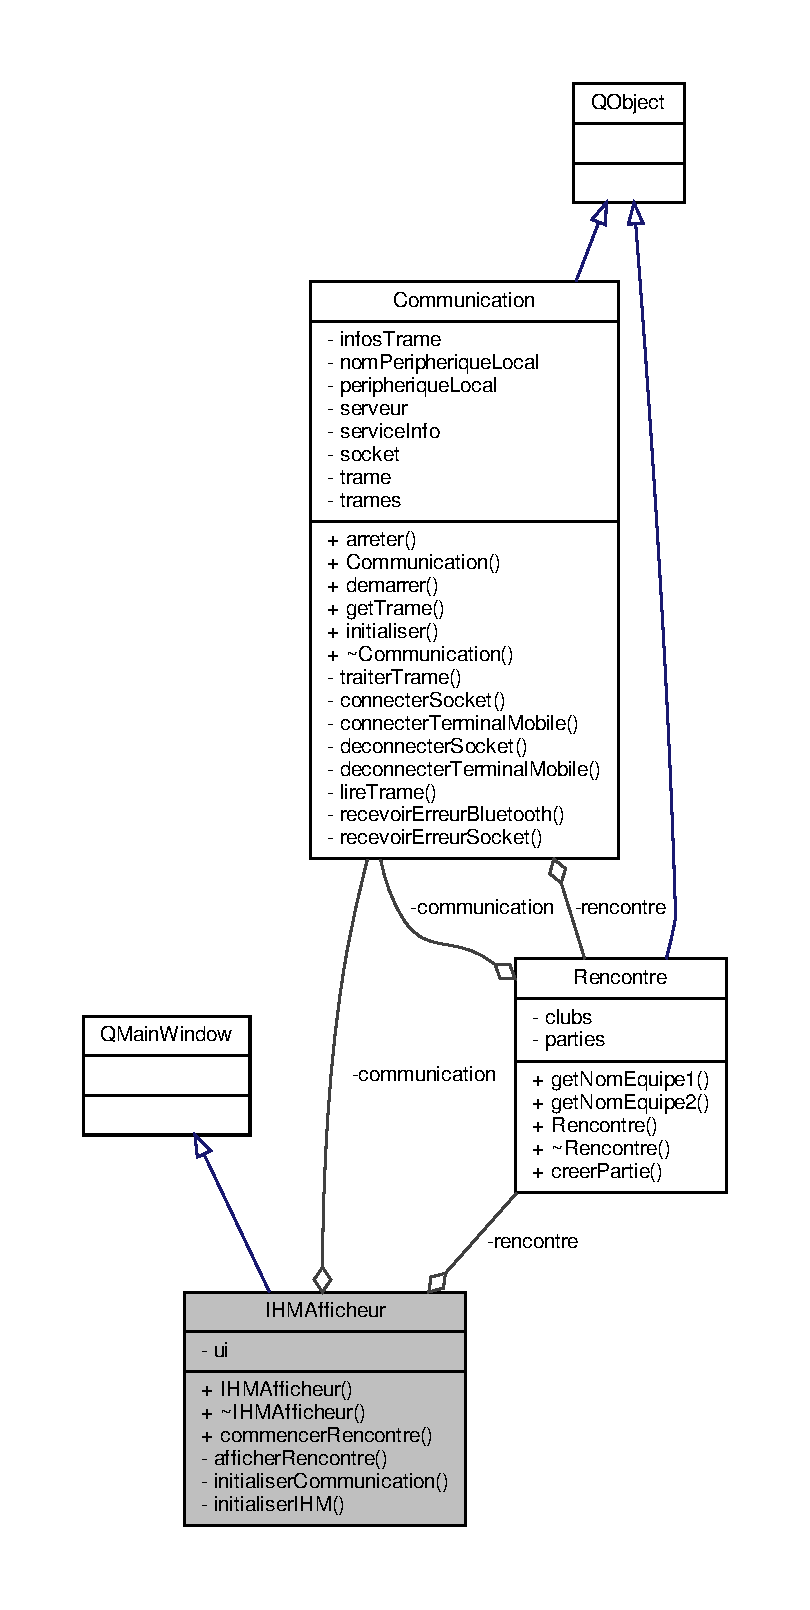
\includegraphics[height=550pt]{class_i_h_m_afficheur__coll__graph}
\end{center}
\end{figure}
\subsubsection*{Connecteurs publics}
\begin{DoxyCompactItemize}
\item 
void \hyperlink{class_i_h_m_afficheur_ad2dc0742d9cdda731a16c570fd6f2434}{commencer\+Rencontre} (Q\+String club1, Q\+String club2)
\begin{DoxyCompactList}\small\item\em Commence une rencontre entre deux clubs. \end{DoxyCompactList}\end{DoxyCompactItemize}
\subsubsection*{Fonctions membres publiques}
\begin{DoxyCompactItemize}
\item 
\hyperlink{class_i_h_m_afficheur_a2fdf6626a1d9c2c635110a6e6ab703f9}{I\+H\+M\+Afficheur} (Q\+Widget $\ast$parent=0)
\begin{DoxyCompactList}\small\item\em Constructeur de la classe \hyperlink{class_i_h_m_afficheur}{I\+H\+M\+Afficheur}. \end{DoxyCompactList}\item 
\hyperlink{class_i_h_m_afficheur_aba47ddf68f3966ed8f5c697b48e352a4}{$\sim$\+I\+H\+M\+Afficheur} ()
\begin{DoxyCompactList}\small\item\em Destructeur de la classe \hyperlink{class_i_h_m_afficheur}{I\+H\+M\+Afficheur}. \end{DoxyCompactList}\end{DoxyCompactItemize}
\subsubsection*{Fonctions membres privées}
\begin{DoxyCompactItemize}
\item 
void \hyperlink{class_i_h_m_afficheur_aec1fee14a130ea53206bf5f8e532b819}{afficher\+Rencontre} ()
\item 
void \hyperlink{class_i_h_m_afficheur_ab7a8db8e7cfa6dc86ab59a07ede75298}{initialiser\+Communication} ()
\begin{DoxyCompactList}\small\item\em Initialise la communication Bluetooth en mode serveur. \end{DoxyCompactList}\item 
void \hyperlink{class_i_h_m_afficheur_a119539fa51bf2e091e77faedf82eb146}{initialiser\+I\+HM} ()
\begin{DoxyCompactList}\small\item\em Initialise les widgets de l\textquotesingle{}I\+HM. \end{DoxyCompactList}\end{DoxyCompactItemize}
\subsubsection*{Attributs privés}
\begin{DoxyCompactItemize}
\item 
\hyperlink{class_communication}{Communication} $\ast$ \hyperlink{class_i_h_m_afficheur_a331b5544e96cc908336a1486b52c379b}{communication}
\item 
\hyperlink{class_rencontre}{Rencontre} $\ast$ \hyperlink{class_i_h_m_afficheur_aef34d340f7ea30f049a98efc47bd9779}{rencontre}
\item 
Ui\+::\+I\+H\+M\+Afficheur $\ast$ \hyperlink{class_i_h_m_afficheur_a26ca43f1ff87b1caa2191adcce444d23}{ui}
\begin{DoxyCompactList}\small\item\em Association vers l\textquotesingle{}interface utilisateur réalisé avec Qt Designer. \end{DoxyCompactList}\end{DoxyCompactItemize}


\subsubsection{Description détaillée}
Déclaration de la classe \hyperlink{class_i_h_m_afficheur}{I\+H\+M\+Afficheur}. 

Cette classe assure l\textquotesingle{}affichage de l\textquotesingle{}écran A\+R\+EA 

Définition à la ligne \hyperlink{_i_h_m_afficheur_8h_source_l00034}{34} du fichier \hyperlink{_i_h_m_afficheur_8h_source}{I\+H\+M\+Afficheur.\+h}.



\subsubsection{Documentation des constructeurs et destructeur}
\mbox{\Hypertarget{class_i_h_m_afficheur_a2fdf6626a1d9c2c635110a6e6ab703f9}\label{class_i_h_m_afficheur_a2fdf6626a1d9c2c635110a6e6ab703f9}} 
\index{I\+H\+M\+Afficheur@{I\+H\+M\+Afficheur}!I\+H\+M\+Afficheur@{I\+H\+M\+Afficheur}}
\index{I\+H\+M\+Afficheur@{I\+H\+M\+Afficheur}!I\+H\+M\+Afficheur@{I\+H\+M\+Afficheur}}
\paragraph{\texorpdfstring{I\+H\+M\+Afficheur()}{IHMAfficheur()}}
{\footnotesize\ttfamily I\+H\+M\+Afficheur\+::\+I\+H\+M\+Afficheur (\begin{DoxyParamCaption}\item[{Q\+Widget $\ast$}]{parent = {\ttfamily 0} }\end{DoxyParamCaption})\hspace{0.3cm}{\ttfamily [explicit]}}



Constructeur de la classe \hyperlink{class_i_h_m_afficheur}{I\+H\+M\+Afficheur}. 


\begin{DoxyParams}{Paramètres}
{\em parent} & L\textquotesingle{}adresse de l\textquotesingle{}objet parent, si nullptr \hyperlink{class_i_h_m_afficheur}{I\+H\+M\+Afficheur} sera la fenêtre principale \\
\hline
\end{DoxyParams}


Définition à la ligne \hyperlink{_i_h_m_afficheur_8cpp_source_l00022}{22} du fichier \hyperlink{_i_h_m_afficheur_8cpp_source}{I\+H\+M\+Afficheur.\+cpp}.



Références \hyperlink{_i_h_m_afficheur_8cpp_source_l00090}{commencer\+Rencontre()}, \hyperlink{_i_h_m_afficheur_8cpp_source_l00074}{initialiser\+Communication()}, et \hyperlink{_i_h_m_afficheur_8cpp_source_l00056}{initialiser\+I\+H\+M()}.


\begin{DoxyCode}
00022                                           : \hyperlink{class_q_main_window}{QMainWindow}(parent), \hyperlink{class_i_h_m_afficheur_a26ca43f1ff87b1caa2191adcce444d23}{ui}(\textcolor{keyword}{new} Ui::IHMAfficheur), 
      \hyperlink{class_i_h_m_afficheur_aef34d340f7ea30f049a98efc47bd9779}{rencontre}(\textcolor{keyword}{nullptr}), \hyperlink{class_i_h_m_afficheur_a331b5544e96cc908336a1486b52c379b}{communication}(\textcolor{keyword}{nullptr})
00023 \{
00024     qDebug() << Q\_FUNC\_INFO;
00025 
00026     \hyperlink{class_i_h_m_afficheur_a119539fa51bf2e091e77faedf82eb146}{initialiserIHM}();
00027 
00028 \textcolor{preprocessor}{    #ifndef TEST\_SANS\_BLUETOOTH}
00029     \hyperlink{class_i_h_m_afficheur_ab7a8db8e7cfa6dc86ab59a07ede75298}{initialiserCommunication}();
00030 \textcolor{preprocessor}{    #endif}
00031 
00032 \textcolor{preprocessor}{    #ifdef TEST\_SANS\_BLUETOOTH}
00033     \hyperlink{class_i_h_m_afficheur_ad2dc0742d9cdda731a16c570fd6f2434}{commencerRencontre}(\textcolor{stringliteral}{"Avignon"}, \textcolor{stringliteral}{"Orange"});
00034 \textcolor{preprocessor}{    #endif}
00035 \}
\end{DoxyCode}
\mbox{\Hypertarget{class_i_h_m_afficheur_aba47ddf68f3966ed8f5c697b48e352a4}\label{class_i_h_m_afficheur_aba47ddf68f3966ed8f5c697b48e352a4}} 
\index{I\+H\+M\+Afficheur@{I\+H\+M\+Afficheur}!````~I\+H\+M\+Afficheur@{$\sim$\+I\+H\+M\+Afficheur}}
\index{````~I\+H\+M\+Afficheur@{$\sim$\+I\+H\+M\+Afficheur}!I\+H\+M\+Afficheur@{I\+H\+M\+Afficheur}}
\paragraph{\texorpdfstring{$\sim$\+I\+H\+M\+Afficheur()}{~IHMAfficheur()}}
{\footnotesize\ttfamily I\+H\+M\+Afficheur\+::$\sim$\+I\+H\+M\+Afficheur (\begin{DoxyParamCaption}{ }\end{DoxyParamCaption})}



Destructeur de la classe \hyperlink{class_i_h_m_afficheur}{I\+H\+M\+Afficheur}. 

Libère les ressources de l\textquotesingle{}application 

Définition à la ligne \hyperlink{_i_h_m_afficheur_8cpp_source_l00043}{43} du fichier \hyperlink{_i_h_m_afficheur_8cpp_source}{I\+H\+M\+Afficheur.\+cpp}.



Références \hyperlink{_i_h_m_afficheur_8h_source_l00040}{rencontre}, et \hyperlink{_i_h_m_afficheur_8h_source_l00039}{ui}.


\begin{DoxyCode}
00044 \{
00045     \textcolor{keywordflow}{if}(\hyperlink{class_i_h_m_afficheur_aef34d340f7ea30f049a98efc47bd9779}{rencontre} != \textcolor{keyword}{nullptr})
00046         \textcolor{keyword}{delete} \hyperlink{class_i_h_m_afficheur_aef34d340f7ea30f049a98efc47bd9779}{rencontre};
00047     \textcolor{keyword}{delete} \hyperlink{class_i_h_m_afficheur_a26ca43f1ff87b1caa2191adcce444d23}{ui};
00048     qDebug() << Q\_FUNC\_INFO;
00049 \}
\end{DoxyCode}


\subsubsection{Documentation des fonctions membres}
\mbox{\Hypertarget{class_i_h_m_afficheur_aec1fee14a130ea53206bf5f8e532b819}\label{class_i_h_m_afficheur_aec1fee14a130ea53206bf5f8e532b819}} 
\index{I\+H\+M\+Afficheur@{I\+H\+M\+Afficheur}!afficher\+Rencontre@{afficher\+Rencontre}}
\index{afficher\+Rencontre@{afficher\+Rencontre}!I\+H\+M\+Afficheur@{I\+H\+M\+Afficheur}}
\paragraph{\texorpdfstring{afficher\+Rencontre()}{afficherRencontre()}}
{\footnotesize\ttfamily void I\+H\+M\+Afficheur\+::afficher\+Rencontre (\begin{DoxyParamCaption}{ }\end{DoxyParamCaption})\hspace{0.3cm}{\ttfamily [private]}}



Définition à la ligne \hyperlink{_i_h_m_afficheur_8cpp_source_l00100}{100} du fichier \hyperlink{_i_h_m_afficheur_8cpp_source}{I\+H\+M\+Afficheur.\+cpp}.



Références \hyperlink{_rencontre_8cpp_source_l00041}{Rencontre\+::get\+Nom\+Equipe1()}, \hyperlink{_rencontre_8cpp_source_l00049}{Rencontre\+::get\+Nom\+Equipe2()}, \hyperlink{_i_h_m_afficheur_8h_source_l00040}{rencontre}, et \hyperlink{_i_h_m_afficheur_8h_source_l00039}{ui}.



Référencé par \hyperlink{_i_h_m_afficheur_8cpp_source_l00090}{commencer\+Rencontre()}.


\begin{DoxyCode}
00101 \{
00102     \hyperlink{class_i_h_m_afficheur_a26ca43f1ff87b1caa2191adcce444d23}{ui}->nomEquipe1->setText(\hyperlink{class_i_h_m_afficheur_aef34d340f7ea30f049a98efc47bd9779}{rencontre}->\hyperlink{class_rencontre_a50df24caf57437d8eaaadae43ff846ec}{getNomEquipe1}());
00103     \hyperlink{class_i_h_m_afficheur_a26ca43f1ff87b1caa2191adcce444d23}{ui}->nomEquipe1->setAlignment(Qt::AlignCenter);
00104     \hyperlink{class_i_h_m_afficheur_a26ca43f1ff87b1caa2191adcce444d23}{ui}->nomEquipe2->setText(\hyperlink{class_i_h_m_afficheur_aef34d340f7ea30f049a98efc47bd9779}{rencontre}->\hyperlink{class_rencontre_ac544f97755480e0e2718d0802d308585}{getNomEquipe2}());
00105     \hyperlink{class_i_h_m_afficheur_a26ca43f1ff87b1caa2191adcce444d23}{ui}->nomEquipe2->setAlignment(Qt::AlignCenter);
00106 \}
\end{DoxyCode}
\mbox{\Hypertarget{class_i_h_m_afficheur_ad2dc0742d9cdda731a16c570fd6f2434}\label{class_i_h_m_afficheur_ad2dc0742d9cdda731a16c570fd6f2434}} 
\index{I\+H\+M\+Afficheur@{I\+H\+M\+Afficheur}!commencer\+Rencontre@{commencer\+Rencontre}}
\index{commencer\+Rencontre@{commencer\+Rencontre}!I\+H\+M\+Afficheur@{I\+H\+M\+Afficheur}}
\paragraph{\texorpdfstring{commencer\+Rencontre}{commencerRencontre}}
{\footnotesize\ttfamily void I\+H\+M\+Afficheur\+::commencer\+Rencontre (\begin{DoxyParamCaption}\item[{Q\+String}]{club1,  }\item[{Q\+String}]{club2 }\end{DoxyParamCaption})\hspace{0.3cm}{\ttfamily [slot]}}



Commence une rencontre entre deux clubs. 


\begin{DoxyParams}{Paramètres}
{\em club1} & \\
\hline
{\em club2} & \\
\hline
\end{DoxyParams}


Définition à la ligne \hyperlink{_i_h_m_afficheur_8cpp_source_l00090}{90} du fichier \hyperlink{_i_h_m_afficheur_8cpp_source}{I\+H\+M\+Afficheur.\+cpp}.



Références \hyperlink{_i_h_m_afficheur_8cpp_source_l00100}{afficher\+Rencontre()}, \hyperlink{_i_h_m_afficheur_8h_source_l00041}{communication}, \hyperlink{_rencontre_8cpp_source_l00041}{Rencontre\+::get\+Nom\+Equipe1()}, \hyperlink{_rencontre_8cpp_source_l00049}{Rencontre\+::get\+Nom\+Equipe2()}, et \hyperlink{_i_h_m_afficheur_8h_source_l00040}{rencontre}.



Référencé par \hyperlink{_i_h_m_afficheur_8cpp_source_l00022}{I\+H\+M\+Afficheur()}, et \hyperlink{_i_h_m_afficheur_8cpp_source_l00074}{initialiser\+Communication()}.


\begin{DoxyCode}
00091 \{
00092     \hyperlink{class_i_h_m_afficheur_aef34d340f7ea30f049a98efc47bd9779}{rencontre} = \textcolor{keyword}{new} \hyperlink{class_rencontre}{Rencontre}(club1, club2);
00093     qDebug() << Q\_FUNC\_INFO << \hyperlink{class_i_h_m_afficheur_aef34d340f7ea30f049a98efc47bd9779}{rencontre}->\hyperlink{class_rencontre_a50df24caf57437d8eaaadae43ff846ec}{getNomEquipe1}() << \textcolor{stringliteral}{"vs"} << 
      \hyperlink{class_i_h_m_afficheur_aef34d340f7ea30f049a98efc47bd9779}{rencontre}->\hyperlink{class_rencontre_ac544f97755480e0e2718d0802d308585}{getNomEquipe2}();
00094 
00095     \hyperlink{class_i_h_m_afficheur_aec1fee14a130ea53206bf5f8e532b819}{afficherRencontre}();
00096 
00097     connect(\hyperlink{class_i_h_m_afficheur_a331b5544e96cc908336a1486b52c379b}{communication}, SIGNAL(creationPartie(QStringList)), 
      \hyperlink{class_i_h_m_afficheur_aef34d340f7ea30f049a98efc47bd9779}{rencontre}, SLOT(creerPartie(QStringList)));
00098 \}
\end{DoxyCode}
\mbox{\Hypertarget{class_i_h_m_afficheur_ab7a8db8e7cfa6dc86ab59a07ede75298}\label{class_i_h_m_afficheur_ab7a8db8e7cfa6dc86ab59a07ede75298}} 
\index{I\+H\+M\+Afficheur@{I\+H\+M\+Afficheur}!initialiser\+Communication@{initialiser\+Communication}}
\index{initialiser\+Communication@{initialiser\+Communication}!I\+H\+M\+Afficheur@{I\+H\+M\+Afficheur}}
\paragraph{\texorpdfstring{initialiser\+Communication()}{initialiserCommunication()}}
{\footnotesize\ttfamily void I\+H\+M\+Afficheur\+::initialiser\+Communication (\begin{DoxyParamCaption}{ }\end{DoxyParamCaption})\hspace{0.3cm}{\ttfamily [private]}}



Initialise la communication Bluetooth en mode serveur. 



Définition à la ligne \hyperlink{_i_h_m_afficheur_8cpp_source_l00074}{74} du fichier \hyperlink{_i_h_m_afficheur_8cpp_source}{I\+H\+M\+Afficheur.\+cpp}.



Références \hyperlink{_i_h_m_afficheur_8cpp_source_l00090}{commencer\+Rencontre()}, \hyperlink{_i_h_m_afficheur_8h_source_l00041}{communication}, et \hyperlink{_communication_8cpp_source_l00073}{Communication\+::demarrer()}.



Référencé par \hyperlink{_i_h_m_afficheur_8cpp_source_l00022}{I\+H\+M\+Afficheur()}.


\begin{DoxyCode}
00075 \{
00076     \hyperlink{class_i_h_m_afficheur_a331b5544e96cc908336a1486b52c379b}{communication} = \textcolor{keyword}{new} \hyperlink{class_communication}{Communication}(\textcolor{keyword}{this});
00077 
00078     connect(\hyperlink{class_i_h_m_afficheur_a331b5544e96cc908336a1486b52c379b}{communication}, SIGNAL(debutRencontre(QString,QString)), \textcolor{keyword}{this}, SLOT(
      \hyperlink{class_i_h_m_afficheur_ad2dc0742d9cdda731a16c570fd6f2434}{commencerRencontre}(QString,QString)));
00079 
00080     \hyperlink{class_i_h_m_afficheur_a331b5544e96cc908336a1486b52c379b}{communication}->\hyperlink{class_communication_af29ea9a1c2ce29436f2331c322f6ebbf}{demarrer}();
00081 \}
\end{DoxyCode}
\mbox{\Hypertarget{class_i_h_m_afficheur_a119539fa51bf2e091e77faedf82eb146}\label{class_i_h_m_afficheur_a119539fa51bf2e091e77faedf82eb146}} 
\index{I\+H\+M\+Afficheur@{I\+H\+M\+Afficheur}!initialiser\+I\+HM@{initialiser\+I\+HM}}
\index{initialiser\+I\+HM@{initialiser\+I\+HM}!I\+H\+M\+Afficheur@{I\+H\+M\+Afficheur}}
\paragraph{\texorpdfstring{initialiser\+I\+H\+M()}{initialiserIHM()}}
{\footnotesize\ttfamily void I\+H\+M\+Afficheur\+::initialiser\+I\+HM (\begin{DoxyParamCaption}{ }\end{DoxyParamCaption})\hspace{0.3cm}{\ttfamily [private]}}



Initialise les widgets de l\textquotesingle{}I\+HM. 



Définition à la ligne \hyperlink{_i_h_m_afficheur_8cpp_source_l00056}{56} du fichier \hyperlink{_i_h_m_afficheur_8cpp_source}{I\+H\+M\+Afficheur.\+cpp}.



Références \hyperlink{_i_h_m_afficheur_8h_source_l00039}{ui}.



Référencé par \hyperlink{_i_h_m_afficheur_8cpp_source_l00022}{I\+H\+M\+Afficheur()}.


\begin{DoxyCode}
00057 \{
00058     \hyperlink{class_i_h_m_afficheur_a26ca43f1ff87b1caa2191adcce444d23}{ui}->setupUi(\textcolor{keyword}{this});
00059 
00060     \hyperlink{class_i_h_m_afficheur_a26ca43f1ff87b1caa2191adcce444d23}{ui}->centralWidget->setStyleSheet(\textcolor{stringliteral}{"QWidget#centralWidget \{background-color: black;\} QLabel \{color:
       white\}"});
00061 
00062     \textcolor{comment}{// Mode debug}
00063     QAction *quitter = \textcolor{keyword}{new} QAction(\textcolor{keyword}{this});
00064     quitter->setShortcut(QKeySequence(QKeySequence(Qt::Key\_Escape)));
00065     addAction(quitter);
00066     connect(quitter, SIGNAL(triggered()), \textcolor{keyword}{this}, SLOT(close()));
00067 \}
\end{DoxyCode}


\subsubsection{Documentation des données membres}
\mbox{\Hypertarget{class_i_h_m_afficheur_a331b5544e96cc908336a1486b52c379b}\label{class_i_h_m_afficheur_a331b5544e96cc908336a1486b52c379b}} 
\index{I\+H\+M\+Afficheur@{I\+H\+M\+Afficheur}!communication@{communication}}
\index{communication@{communication}!I\+H\+M\+Afficheur@{I\+H\+M\+Afficheur}}
\paragraph{\texorpdfstring{communication}{communication}}
{\footnotesize\ttfamily \hyperlink{class_communication}{Communication}$\ast$ I\+H\+M\+Afficheur\+::communication\hspace{0.3cm}{\ttfamily [private]}}



Définition à la ligne \hyperlink{_i_h_m_afficheur_8h_source_l00041}{41} du fichier \hyperlink{_i_h_m_afficheur_8h_source}{I\+H\+M\+Afficheur.\+h}.



Référencé par \hyperlink{_i_h_m_afficheur_8cpp_source_l00090}{commencer\+Rencontre()}, et \hyperlink{_i_h_m_afficheur_8cpp_source_l00074}{initialiser\+Communication()}.

\mbox{\Hypertarget{class_i_h_m_afficheur_aef34d340f7ea30f049a98efc47bd9779}\label{class_i_h_m_afficheur_aef34d340f7ea30f049a98efc47bd9779}} 
\index{I\+H\+M\+Afficheur@{I\+H\+M\+Afficheur}!rencontre@{rencontre}}
\index{rencontre@{rencontre}!I\+H\+M\+Afficheur@{I\+H\+M\+Afficheur}}
\paragraph{\texorpdfstring{rencontre}{rencontre}}
{\footnotesize\ttfamily \hyperlink{class_rencontre}{Rencontre}$\ast$ I\+H\+M\+Afficheur\+::rencontre\hspace{0.3cm}{\ttfamily [private]}}



Définition à la ligne \hyperlink{_i_h_m_afficheur_8h_source_l00040}{40} du fichier \hyperlink{_i_h_m_afficheur_8h_source}{I\+H\+M\+Afficheur.\+h}.



Référencé par \hyperlink{_i_h_m_afficheur_8cpp_source_l00100}{afficher\+Rencontre()}, \hyperlink{_i_h_m_afficheur_8cpp_source_l00090}{commencer\+Rencontre()}, et \hyperlink{_i_h_m_afficheur_8cpp_source_l00043}{$\sim$\+I\+H\+M\+Afficheur()}.

\mbox{\Hypertarget{class_i_h_m_afficheur_a26ca43f1ff87b1caa2191adcce444d23}\label{class_i_h_m_afficheur_a26ca43f1ff87b1caa2191adcce444d23}} 
\index{I\+H\+M\+Afficheur@{I\+H\+M\+Afficheur}!ui@{ui}}
\index{ui@{ui}!I\+H\+M\+Afficheur@{I\+H\+M\+Afficheur}}
\paragraph{\texorpdfstring{ui}{ui}}
{\footnotesize\ttfamily Ui\+::\+I\+H\+M\+Afficheur$\ast$ I\+H\+M\+Afficheur\+::ui\hspace{0.3cm}{\ttfamily [private]}}



Association vers l\textquotesingle{}interface utilisateur réalisé avec Qt Designer. 



Définition à la ligne \hyperlink{_i_h_m_afficheur_8h_source_l00039}{39} du fichier \hyperlink{_i_h_m_afficheur_8h_source}{I\+H\+M\+Afficheur.\+h}.



Référencé par \hyperlink{_i_h_m_afficheur_8cpp_source_l00100}{afficher\+Rencontre()}, \hyperlink{_i_h_m_afficheur_8cpp_source_l00056}{initialiser\+I\+H\+M()}, et \hyperlink{_i_h_m_afficheur_8cpp_source_l00043}{$\sim$\+I\+H\+M\+Afficheur()}.



La documentation de cette classe a été générée à partir des fichiers suivants \+:\begin{DoxyCompactItemize}
\item 
\hyperlink{_i_h_m_afficheur_8h}{I\+H\+M\+Afficheur.\+h}\item 
\hyperlink{_i_h_m_afficheur_8cpp}{I\+H\+M\+Afficheur.\+cpp}\end{DoxyCompactItemize}

\hypertarget{class_joueur}{}\subsection{Référence de la classe Joueur}
\label{class_joueur}\index{Joueur@{Joueur}}


{\ttfamily \#include $<$Joueur.\+h$>$}



Graphe de collaboration de Joueur\+:
\nopagebreak
\begin{figure}[H]
\begin{center}
\leavevmode
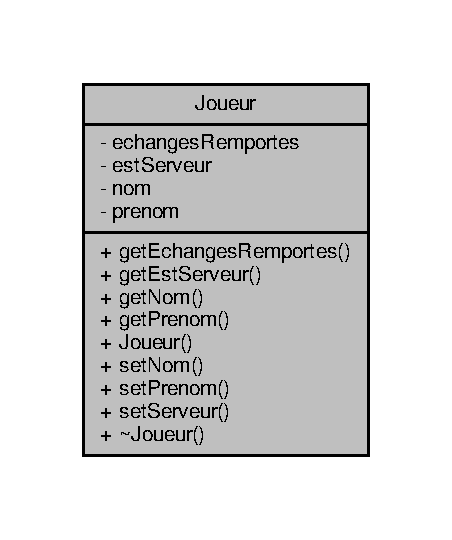
\includegraphics[width=217pt]{class_joueur__coll__graph}
\end{center}
\end{figure}
\subsubsection*{Fonctions membres publiques}
\begin{DoxyCompactItemize}
\item 
int \hyperlink{class_joueur_affde221fc6d6bf633991fff4f11dd62b}{get\+Echanges\+Remportes} () const
\item 
bool \hyperlink{class_joueur_a7bf0e45b6600ae3a68b4afdad6d884b7}{get\+Est\+Serveur} () const
\item 
Q\+String \hyperlink{class_joueur_a1d7082ab1f926eae1bd6834e901751a7}{get\+Nom} () const
\item 
Q\+String \hyperlink{class_joueur_ade527085b285ce86ea9e369bc9959032}{get\+Prenom} () const
\item 
\hyperlink{class_joueur_a75f73a73741b0faa59c75fc98b872765}{Joueur} (Q\+String \hyperlink{class_joueur_ab06d7f1e6b482299bb03919e0cd2166d}{nom}=\char`\"{}nom\+Joueur\char`\"{}, Q\+String \hyperlink{class_joueur_a96d4237143c2e57b8025c4e116e95909}{prenom}=\char`\"{}Prenom\+Joueur\char`\"{})
\item 
void \hyperlink{class_joueur_a30fdb194cbf6d7c378d173cc133fc23e}{set\+Nom} (Q\+String \&n)
\item 
void \hyperlink{class_joueur_a1425ea57a1f030a26d9beb1244e6caa2}{set\+Prenom} (Q\+String \&p)
\item 
void \hyperlink{class_joueur_aea42f5af160c61130d5252796378ad4f}{set\+Serveur} (bool \&e)
\item 
\hyperlink{class_joueur_a9fb594f755601ee77ce5884c4c0861f3}{$\sim$\+Joueur} ()
\end{DoxyCompactItemize}
\subsubsection*{Attributs privés}
\begin{DoxyCompactItemize}
\item 
int \hyperlink{class_joueur_a23ab203e6bbfc1b2679a8457b99206dc}{echanges\+Remportes}
\item 
bool \hyperlink{class_joueur_ac22161c9510ed38d6c65cdf6315737a5}{est\+Serveur}
\item 
Q\+String \hyperlink{class_joueur_ab06d7f1e6b482299bb03919e0cd2166d}{nom}
\item 
Q\+String \hyperlink{class_joueur_a96d4237143c2e57b8025c4e116e95909}{prenom}
\end{DoxyCompactItemize}


\subsubsection{Description détaillée}


Définition à la ligne \hyperlink{_joueur_8h_source_l00015}{15} du fichier \hyperlink{_joueur_8h_source}{Joueur.\+h}.



\subsubsection{Documentation des constructeurs et destructeur}
\mbox{\Hypertarget{class_joueur_a75f73a73741b0faa59c75fc98b872765}\label{class_joueur_a75f73a73741b0faa59c75fc98b872765}} 
\index{Joueur@{Joueur}!Joueur@{Joueur}}
\index{Joueur@{Joueur}!Joueur@{Joueur}}
\paragraph{\texorpdfstring{Joueur()}{Joueur()}}
{\footnotesize\ttfamily Joueur\+::\+Joueur (\begin{DoxyParamCaption}\item[{Q\+String}]{nom = {\ttfamily \char`\"{}nomJoueur\char`\"{}},  }\item[{Q\+String}]{prenom = {\ttfamily \char`\"{}PrenomJoueur\char`\"{}} }\end{DoxyParamCaption})}



Définition à la ligne \hyperlink{_joueur_8cpp_source_l00013}{13} du fichier \hyperlink{_joueur_8cpp_source}{Joueur.\+cpp}.



Références \hyperlink{_joueur_8h_source_l00019}{prenom}.


\begin{DoxyCode}
00013                                           : \hyperlink{class_joueur_ab06d7f1e6b482299bb03919e0cd2166d}{nom}(\hyperlink{class_joueur_ab06d7f1e6b482299bb03919e0cd2166d}{nom}), \hyperlink{class_joueur_a96d4237143c2e57b8025c4e116e95909}{prenom}(\hyperlink{class_joueur_a96d4237143c2e57b8025c4e116e95909}{prenom}), 
      \hyperlink{class_joueur_ac22161c9510ed38d6c65cdf6315737a5}{estServeur}(\textcolor{keyword}{false}), \hyperlink{class_joueur_a23ab203e6bbfc1b2679a8457b99206dc}{echangesRemportes}(0)
00014 \{
00015     qDebug() << Q\_FUNC\_INFO << \hyperlink{class_joueur_ab06d7f1e6b482299bb03919e0cd2166d}{nom} << \hyperlink{class_joueur_a96d4237143c2e57b8025c4e116e95909}{prenom};
00016 \}
\end{DoxyCode}
\mbox{\Hypertarget{class_joueur_a9fb594f755601ee77ce5884c4c0861f3}\label{class_joueur_a9fb594f755601ee77ce5884c4c0861f3}} 
\index{Joueur@{Joueur}!````~Joueur@{$\sim$\+Joueur}}
\index{````~Joueur@{$\sim$\+Joueur}!Joueur@{Joueur}}
\paragraph{\texorpdfstring{$\sim$\+Joueur()}{~Joueur()}}
{\footnotesize\ttfamily Joueur\+::$\sim$\+Joueur (\begin{DoxyParamCaption}{ }\end{DoxyParamCaption})}



Définition à la ligne \hyperlink{_joueur_8cpp_source_l00018}{18} du fichier \hyperlink{_joueur_8cpp_source}{Joueur.\+cpp}.


\begin{DoxyCode}
00019 \{
00020     qDebug() << Q\_FUNC\_INFO;
00021 \}
\end{DoxyCode}


\subsubsection{Documentation des fonctions membres}
\mbox{\Hypertarget{class_joueur_affde221fc6d6bf633991fff4f11dd62b}\label{class_joueur_affde221fc6d6bf633991fff4f11dd62b}} 
\index{Joueur@{Joueur}!get\+Echanges\+Remportes@{get\+Echanges\+Remportes}}
\index{get\+Echanges\+Remportes@{get\+Echanges\+Remportes}!Joueur@{Joueur}}
\paragraph{\texorpdfstring{get\+Echanges\+Remportes()}{getEchangesRemportes()}}
{\footnotesize\ttfamily int Joueur\+::get\+Echanges\+Remportes (\begin{DoxyParamCaption}{ }\end{DoxyParamCaption}) const}



Définition à la ligne \hyperlink{_joueur_8cpp_source_l00053}{53} du fichier \hyperlink{_joueur_8cpp_source}{Joueur.\+cpp}.



Références \hyperlink{_joueur_8h_source_l00021}{echanges\+Remportes}.


\begin{DoxyCode}
00054 \{
00055     \textcolor{keywordflow}{return} \hyperlink{class_joueur_a23ab203e6bbfc1b2679a8457b99206dc}{echangesRemportes};
00056 \}
\end{DoxyCode}
\mbox{\Hypertarget{class_joueur_a7bf0e45b6600ae3a68b4afdad6d884b7}\label{class_joueur_a7bf0e45b6600ae3a68b4afdad6d884b7}} 
\index{Joueur@{Joueur}!get\+Est\+Serveur@{get\+Est\+Serveur}}
\index{get\+Est\+Serveur@{get\+Est\+Serveur}!Joueur@{Joueur}}
\paragraph{\texorpdfstring{get\+Est\+Serveur()}{getEstServeur()}}
{\footnotesize\ttfamily bool Joueur\+::get\+Est\+Serveur (\begin{DoxyParamCaption}{ }\end{DoxyParamCaption}) const}



Définition à la ligne \hyperlink{_joueur_8cpp_source_l00043}{43} du fichier \hyperlink{_joueur_8cpp_source}{Joueur.\+cpp}.



Références \hyperlink{_joueur_8h_source_l00020}{est\+Serveur}.


\begin{DoxyCode}
00044 \{
00045     \textcolor{keywordflow}{return} this->\hyperlink{class_joueur_ac22161c9510ed38d6c65cdf6315737a5}{estServeur};
00046 \}
\end{DoxyCode}
\mbox{\Hypertarget{class_joueur_a1d7082ab1f926eae1bd6834e901751a7}\label{class_joueur_a1d7082ab1f926eae1bd6834e901751a7}} 
\index{Joueur@{Joueur}!get\+Nom@{get\+Nom}}
\index{get\+Nom@{get\+Nom}!Joueur@{Joueur}}
\paragraph{\texorpdfstring{get\+Nom()}{getNom()}}
{\footnotesize\ttfamily Q\+String Joueur\+::get\+Nom (\begin{DoxyParamCaption}{ }\end{DoxyParamCaption}) const}



Définition à la ligne \hyperlink{_joueur_8cpp_source_l00023}{23} du fichier \hyperlink{_joueur_8cpp_source}{Joueur.\+cpp}.



Références \hyperlink{_joueur_8h_source_l00018}{nom}.


\begin{DoxyCode}
00024 \{
00025     \textcolor{keywordflow}{return} this->\hyperlink{class_joueur_ab06d7f1e6b482299bb03919e0cd2166d}{nom};
00026 \}
\end{DoxyCode}
\mbox{\Hypertarget{class_joueur_ade527085b285ce86ea9e369bc9959032}\label{class_joueur_ade527085b285ce86ea9e369bc9959032}} 
\index{Joueur@{Joueur}!get\+Prenom@{get\+Prenom}}
\index{get\+Prenom@{get\+Prenom}!Joueur@{Joueur}}
\paragraph{\texorpdfstring{get\+Prenom()}{getPrenom()}}
{\footnotesize\ttfamily Q\+String Joueur\+::get\+Prenom (\begin{DoxyParamCaption}{ }\end{DoxyParamCaption}) const}



Définition à la ligne \hyperlink{_joueur_8cpp_source_l00033}{33} du fichier \hyperlink{_joueur_8cpp_source}{Joueur.\+cpp}.



Références \hyperlink{_joueur_8h_source_l00019}{prenom}.


\begin{DoxyCode}
00034 \{
00035     \textcolor{keywordflow}{return} this->\hyperlink{class_joueur_a96d4237143c2e57b8025c4e116e95909}{prenom};
00036 \}
\end{DoxyCode}
\mbox{\Hypertarget{class_joueur_a30fdb194cbf6d7c378d173cc133fc23e}\label{class_joueur_a30fdb194cbf6d7c378d173cc133fc23e}} 
\index{Joueur@{Joueur}!set\+Nom@{set\+Nom}}
\index{set\+Nom@{set\+Nom}!Joueur@{Joueur}}
\paragraph{\texorpdfstring{set\+Nom()}{setNom()}}
{\footnotesize\ttfamily void Joueur\+::set\+Nom (\begin{DoxyParamCaption}\item[{Q\+String \&}]{n }\end{DoxyParamCaption})}



Définition à la ligne \hyperlink{_joueur_8cpp_source_l00028}{28} du fichier \hyperlink{_joueur_8cpp_source}{Joueur.\+cpp}.



Références \hyperlink{_joueur_8h_source_l00018}{nom}.


\begin{DoxyCode}
00029 \{
00030     \hyperlink{class_joueur_ab06d7f1e6b482299bb03919e0cd2166d}{nom} = n;
00031 \}
\end{DoxyCode}
\mbox{\Hypertarget{class_joueur_a1425ea57a1f030a26d9beb1244e6caa2}\label{class_joueur_a1425ea57a1f030a26d9beb1244e6caa2}} 
\index{Joueur@{Joueur}!set\+Prenom@{set\+Prenom}}
\index{set\+Prenom@{set\+Prenom}!Joueur@{Joueur}}
\paragraph{\texorpdfstring{set\+Prenom()}{setPrenom()}}
{\footnotesize\ttfamily void Joueur\+::set\+Prenom (\begin{DoxyParamCaption}\item[{Q\+String \&}]{p }\end{DoxyParamCaption})}



Définition à la ligne \hyperlink{_joueur_8cpp_source_l00038}{38} du fichier \hyperlink{_joueur_8cpp_source}{Joueur.\+cpp}.



Références \hyperlink{_joueur_8h_source_l00019}{prenom}.


\begin{DoxyCode}
00039 \{
00040     \hyperlink{class_joueur_a96d4237143c2e57b8025c4e116e95909}{prenom} = p;
00041 \}
\end{DoxyCode}
\mbox{\Hypertarget{class_joueur_aea42f5af160c61130d5252796378ad4f}\label{class_joueur_aea42f5af160c61130d5252796378ad4f}} 
\index{Joueur@{Joueur}!set\+Serveur@{set\+Serveur}}
\index{set\+Serveur@{set\+Serveur}!Joueur@{Joueur}}
\paragraph{\texorpdfstring{set\+Serveur()}{setServeur()}}
{\footnotesize\ttfamily void Joueur\+::set\+Serveur (\begin{DoxyParamCaption}\item[{bool \&}]{e }\end{DoxyParamCaption})}



Définition à la ligne \hyperlink{_joueur_8cpp_source_l00048}{48} du fichier \hyperlink{_joueur_8cpp_source}{Joueur.\+cpp}.



Références \hyperlink{_joueur_8h_source_l00020}{est\+Serveur}.


\begin{DoxyCode}
00049 \{
00050     \hyperlink{class_joueur_ac22161c9510ed38d6c65cdf6315737a5}{estServeur} = e;
00051 \}
\end{DoxyCode}


\subsubsection{Documentation des données membres}
\mbox{\Hypertarget{class_joueur_a23ab203e6bbfc1b2679a8457b99206dc}\label{class_joueur_a23ab203e6bbfc1b2679a8457b99206dc}} 
\index{Joueur@{Joueur}!echanges\+Remportes@{echanges\+Remportes}}
\index{echanges\+Remportes@{echanges\+Remportes}!Joueur@{Joueur}}
\paragraph{\texorpdfstring{echanges\+Remportes}{echangesRemportes}}
{\footnotesize\ttfamily int Joueur\+::echanges\+Remportes\hspace{0.3cm}{\ttfamily [private]}}



Définition à la ligne \hyperlink{_joueur_8h_source_l00021}{21} du fichier \hyperlink{_joueur_8h_source}{Joueur.\+h}.



Référencé par \hyperlink{_joueur_8cpp_source_l00053}{get\+Echanges\+Remportes()}.

\mbox{\Hypertarget{class_joueur_ac22161c9510ed38d6c65cdf6315737a5}\label{class_joueur_ac22161c9510ed38d6c65cdf6315737a5}} 
\index{Joueur@{Joueur}!est\+Serveur@{est\+Serveur}}
\index{est\+Serveur@{est\+Serveur}!Joueur@{Joueur}}
\paragraph{\texorpdfstring{est\+Serveur}{estServeur}}
{\footnotesize\ttfamily bool Joueur\+::est\+Serveur\hspace{0.3cm}{\ttfamily [private]}}



Définition à la ligne \hyperlink{_joueur_8h_source_l00020}{20} du fichier \hyperlink{_joueur_8h_source}{Joueur.\+h}.



Référencé par \hyperlink{_joueur_8cpp_source_l00043}{get\+Est\+Serveur()}, et \hyperlink{_joueur_8cpp_source_l00048}{set\+Serveur()}.

\mbox{\Hypertarget{class_joueur_ab06d7f1e6b482299bb03919e0cd2166d}\label{class_joueur_ab06d7f1e6b482299bb03919e0cd2166d}} 
\index{Joueur@{Joueur}!nom@{nom}}
\index{nom@{nom}!Joueur@{Joueur}}
\paragraph{\texorpdfstring{nom}{nom}}
{\footnotesize\ttfamily Q\+String Joueur\+::nom\hspace{0.3cm}{\ttfamily [private]}}



Définition à la ligne \hyperlink{_joueur_8h_source_l00018}{18} du fichier \hyperlink{_joueur_8h_source}{Joueur.\+h}.



Référencé par \hyperlink{_joueur_8cpp_source_l00023}{get\+Nom()}, et \hyperlink{_joueur_8cpp_source_l00028}{set\+Nom()}.

\mbox{\Hypertarget{class_joueur_a96d4237143c2e57b8025c4e116e95909}\label{class_joueur_a96d4237143c2e57b8025c4e116e95909}} 
\index{Joueur@{Joueur}!prenom@{prenom}}
\index{prenom@{prenom}!Joueur@{Joueur}}
\paragraph{\texorpdfstring{prenom}{prenom}}
{\footnotesize\ttfamily Q\+String Joueur\+::prenom\hspace{0.3cm}{\ttfamily [private]}}



Définition à la ligne \hyperlink{_joueur_8h_source_l00019}{19} du fichier \hyperlink{_joueur_8h_source}{Joueur.\+h}.



Référencé par \hyperlink{_joueur_8cpp_source_l00033}{get\+Prenom()}, \hyperlink{_joueur_8cpp_source_l00013}{Joueur()}, et \hyperlink{_joueur_8cpp_source_l00038}{set\+Prenom()}.



La documentation de cette classe a été générée à partir des fichiers suivants \+:\begin{DoxyCompactItemize}
\item 
\hyperlink{_joueur_8h}{Joueur.\+h}\item 
\hyperlink{_joueur_8cpp}{Joueur.\+cpp}\end{DoxyCompactItemize}

\hypertarget{class_partie}{}\subsection{Référence de la classe Partie}
\label{class_partie}\index{Partie@{Partie}}


{\ttfamily \#include $<$Partie.\+h$>$}



Graphe de collaboration de Partie\+:
\nopagebreak
\begin{figure}[H]
\begin{center}
\leavevmode
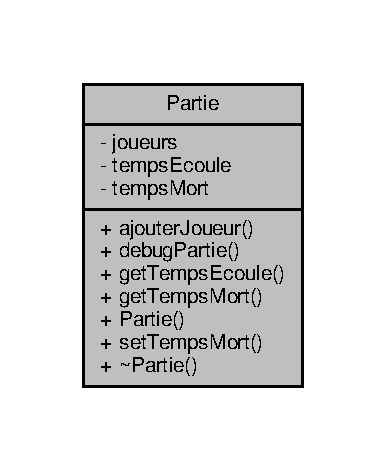
\includegraphics[width=185pt]{class_partie__coll__graph}
\end{center}
\end{figure}
\subsubsection*{Fonctions membres publiques}
\begin{DoxyCompactItemize}
\item 
void \hyperlink{class_partie_ab9900d3b66d9ac7eabc837c790faa6b8}{ajouter\+Joueur} (Q\+String \&nom\+Joueur, Q\+String \&prenom\+Joueur)
\item 
void \hyperlink{class_partie_aea05906078462b32bf08a3172ab14328}{debug\+Partie} ()
\item 
int \hyperlink{class_partie_ab5bb77bcbdb9a145016ebb4ff2bf6c38}{get\+Temps\+Ecoule} () const
\item 
int \hyperlink{class_partie_ad78c6daffd7a676ce6c0a8e511991a75}{get\+Temps\+Mort} () const
\item 
\hyperlink{class_partie_ae1a2da8080f9f51bdd7e9d864080444c}{Partie} (\hyperlink{class_joueur}{Joueur} joueurA=\hyperlink{class_joueur}{Joueur}(\char`\"{}nom\+Joueur1\char`\"{}, \char`\"{}prenom\+Joueur1\char`\"{}), Joueur joueurB=\hyperlink{class_joueur}{Joueur}(\char`\"{}nom\+Joueur2\char`\"{}, \char`\"{}prenom\+Joueur2\char`\"{}))
\item 
void \hyperlink{class_partie_a4c9c799ba4057c15c0600bdf8b7f296f}{set\+Temps\+Mort} (int \&t)
\item 
\hyperlink{class_partie_ae4afeb7336bb84427272cfb7018b5e3d}{$\sim$\+Partie} ()
\end{DoxyCompactItemize}
\subsubsection*{Attributs privés}
\begin{DoxyCompactItemize}
\item 
Q\+Vector$<$ \hyperlink{class_joueur}{Joueur} $>$ \hyperlink{class_partie_a98fa2810599b3eb46d57df2b5836a3f4}{joueurs}
\item 
int \hyperlink{class_partie_a58664212ddb4954a59298f1de8256477}{temps\+Ecoule}
\item 
int \hyperlink{class_partie_a55a5e6e0b757d74fa9aceefa7228ead9}{temps\+Mort}
\end{DoxyCompactItemize}


\subsubsection{Description détaillée}


Définition à la ligne \hyperlink{_partie_8h_source_l00016}{16} du fichier \hyperlink{_partie_8h_source}{Partie.\+h}.



\subsubsection{Documentation des constructeurs et destructeur}
\mbox{\Hypertarget{class_partie_ae1a2da8080f9f51bdd7e9d864080444c}\label{class_partie_ae1a2da8080f9f51bdd7e9d864080444c}} 
\index{Partie@{Partie}!Partie@{Partie}}
\index{Partie@{Partie}!Partie@{Partie}}
\paragraph{\texorpdfstring{Partie()}{Partie()}}
{\footnotesize\ttfamily Partie\+::\+Partie (\begin{DoxyParamCaption}\item[{\hyperlink{class_joueur}{Joueur}}]{joueurA = {\ttfamily \hyperlink{class_joueur}{Joueur}(\char`\"{}nomJoueur1\char`\"{},~\char`\"{}prenomJoueur1\char`\"{})},  }\item[{\hyperlink{class_joueur}{Joueur}}]{joueurB = {\ttfamily \hyperlink{class_joueur}{Joueur}(\char`\"{}nomJoueur2\char`\"{},~\char`\"{}prenomJoueur2\char`\"{})} }\end{DoxyParamCaption})}



Définition à la ligne \hyperlink{_partie_8cpp_source_l00013}{13} du fichier \hyperlink{_partie_8cpp_source}{Partie.\+cpp}.



Références \hyperlink{_partie_8h_source_l00020}{temps\+Ecoule}, et \hyperlink{_partie_8h_source_l00021}{temps\+Mort}.


\begin{DoxyCode}
00013                                              : \hyperlink{class_partie_a98fa2810599b3eb46d57df2b5836a3f4}{joueurs}(\{joueurA, joueurB\}), 
      \hyperlink{class_partie_a58664212ddb4954a59298f1de8256477}{tempsEcoule}(0), \hyperlink{class_partie_a55a5e6e0b757d74fa9aceefa7228ead9}{tempsMort}(0)
00014 \{
00015     qDebug() << Q\_FUNC\_INFO << joueurA.\hyperlink{class_joueur_a1d7082ab1f926eae1bd6834e901751a7}{getNom}() << joueurA.\hyperlink{class_joueur_ade527085b285ce86ea9e369bc9959032}{getPrenom}() << \textcolor{stringliteral}{"vs"} << joueurB.
      \hyperlink{class_joueur_a1d7082ab1f926eae1bd6834e901751a7}{getNom}() << joueurB.\hyperlink{class_joueur_ade527085b285ce86ea9e369bc9959032}{getPrenom}();
00016 \}
\end{DoxyCode}
\mbox{\Hypertarget{class_partie_ae4afeb7336bb84427272cfb7018b5e3d}\label{class_partie_ae4afeb7336bb84427272cfb7018b5e3d}} 
\index{Partie@{Partie}!````~Partie@{$\sim$\+Partie}}
\index{````~Partie@{$\sim$\+Partie}!Partie@{Partie}}
\paragraph{\texorpdfstring{$\sim$\+Partie()}{~Partie()}}
{\footnotesize\ttfamily Partie\+::$\sim$\+Partie (\begin{DoxyParamCaption}{ }\end{DoxyParamCaption})}



Définition à la ligne \hyperlink{_partie_8cpp_source_l00018}{18} du fichier \hyperlink{_partie_8cpp_source}{Partie.\+cpp}.


\begin{DoxyCode}
00019 \{
00020     qDebug() << Q\_FUNC\_INFO;
00021 \}
\end{DoxyCode}


\subsubsection{Documentation des fonctions membres}
\mbox{\Hypertarget{class_partie_ab9900d3b66d9ac7eabc837c790faa6b8}\label{class_partie_ab9900d3b66d9ac7eabc837c790faa6b8}} 
\index{Partie@{Partie}!ajouter\+Joueur@{ajouter\+Joueur}}
\index{ajouter\+Joueur@{ajouter\+Joueur}!Partie@{Partie}}
\paragraph{\texorpdfstring{ajouter\+Joueur()}{ajouterJoueur()}}
{\footnotesize\ttfamily void Partie\+::ajouter\+Joueur (\begin{DoxyParamCaption}\item[{Q\+String \&}]{nom\+Joueur,  }\item[{Q\+String \&}]{prenom\+Joueur }\end{DoxyParamCaption})}



Définition à la ligne \hyperlink{_partie_8cpp_source_l00038}{38} du fichier \hyperlink{_partie_8cpp_source}{Partie.\+cpp}.



Références \hyperlink{_partie_8h_source_l00019}{joueurs}.


\begin{DoxyCode}
00039 \{
00040     qDebug() << Q\_FUNC\_INFO << nomJoueur << prenomJoueur;
00041     \hyperlink{class_joueur}{Joueur} joueur(nomJoueur,prenomJoueur);
00042     \hyperlink{class_partie_a98fa2810599b3eb46d57df2b5836a3f4}{joueurs}.push\_back(joueur);
00043 \}
\end{DoxyCode}
\mbox{\Hypertarget{class_partie_aea05906078462b32bf08a3172ab14328}\label{class_partie_aea05906078462b32bf08a3172ab14328}} 
\index{Partie@{Partie}!debug\+Partie@{debug\+Partie}}
\index{debug\+Partie@{debug\+Partie}!Partie@{Partie}}
\paragraph{\texorpdfstring{debug\+Partie()}{debugPartie()}}
{\footnotesize\ttfamily void Partie\+::debug\+Partie (\begin{DoxyParamCaption}{ }\end{DoxyParamCaption})}



Définition à la ligne \hyperlink{_partie_8cpp_source_l00045}{45} du fichier \hyperlink{_partie_8cpp_source}{Partie.\+cpp}.



Références \hyperlink{_partie_8h_source_l00019}{joueurs}.


\begin{DoxyCode}
00046 \{
00047     qDebug() << \textcolor{stringliteral}{"Nb joueurs : "} << \hyperlink{class_partie_a98fa2810599b3eb46d57df2b5836a3f4}{joueurs}.size();
00048     qDebug() << \textcolor{stringliteral}{"Partie existente"} << \hyperlink{class_partie_a98fa2810599b3eb46d57df2b5836a3f4}{joueurs}[0].getNom() << \hyperlink{class_partie_a98fa2810599b3eb46d57df2b5836a3f4}{joueurs}[0].getPrenom() << \textcolor{stringliteral}{"vs"} <
      < \hyperlink{class_partie_a98fa2810599b3eb46d57df2b5836a3f4}{joueurs}[1].getNom() << \hyperlink{class_partie_a98fa2810599b3eb46d57df2b5836a3f4}{joueurs}[1].getPrenom();
00049 \}
\end{DoxyCode}
\mbox{\Hypertarget{class_partie_ab5bb77bcbdb9a145016ebb4ff2bf6c38}\label{class_partie_ab5bb77bcbdb9a145016ebb4ff2bf6c38}} 
\index{Partie@{Partie}!get\+Temps\+Ecoule@{get\+Temps\+Ecoule}}
\index{get\+Temps\+Ecoule@{get\+Temps\+Ecoule}!Partie@{Partie}}
\paragraph{\texorpdfstring{get\+Temps\+Ecoule()}{getTempsEcoule()}}
{\footnotesize\ttfamily int Partie\+::get\+Temps\+Ecoule (\begin{DoxyParamCaption}{ }\end{DoxyParamCaption}) const}



Définition à la ligne \hyperlink{_partie_8cpp_source_l00023}{23} du fichier \hyperlink{_partie_8cpp_source}{Partie.\+cpp}.



Références \hyperlink{_partie_8h_source_l00020}{temps\+Ecoule}.


\begin{DoxyCode}
00024 \{
00025     \textcolor{keywordflow}{return} this->\hyperlink{class_partie_a58664212ddb4954a59298f1de8256477}{tempsEcoule};
00026 \}
\end{DoxyCode}
\mbox{\Hypertarget{class_partie_ad78c6daffd7a676ce6c0a8e511991a75}\label{class_partie_ad78c6daffd7a676ce6c0a8e511991a75}} 
\index{Partie@{Partie}!get\+Temps\+Mort@{get\+Temps\+Mort}}
\index{get\+Temps\+Mort@{get\+Temps\+Mort}!Partie@{Partie}}
\paragraph{\texorpdfstring{get\+Temps\+Mort()}{getTempsMort()}}
{\footnotesize\ttfamily int Partie\+::get\+Temps\+Mort (\begin{DoxyParamCaption}{ }\end{DoxyParamCaption}) const}



Définition à la ligne \hyperlink{_partie_8cpp_source_l00033}{33} du fichier \hyperlink{_partie_8cpp_source}{Partie.\+cpp}.



Références \hyperlink{_partie_8h_source_l00021}{temps\+Mort}.


\begin{DoxyCode}
00034 \{
00035     \textcolor{keywordflow}{return} this->\hyperlink{class_partie_a55a5e6e0b757d74fa9aceefa7228ead9}{tempsMort};
00036 \}
\end{DoxyCode}
\mbox{\Hypertarget{class_partie_a4c9c799ba4057c15c0600bdf8b7f296f}\label{class_partie_a4c9c799ba4057c15c0600bdf8b7f296f}} 
\index{Partie@{Partie}!set\+Temps\+Mort@{set\+Temps\+Mort}}
\index{set\+Temps\+Mort@{set\+Temps\+Mort}!Partie@{Partie}}
\paragraph{\texorpdfstring{set\+Temps\+Mort()}{setTempsMort()}}
{\footnotesize\ttfamily void Partie\+::set\+Temps\+Mort (\begin{DoxyParamCaption}\item[{int \&}]{t }\end{DoxyParamCaption})}



Définition à la ligne \hyperlink{_partie_8cpp_source_l00028}{28} du fichier \hyperlink{_partie_8cpp_source}{Partie.\+cpp}.



Références \hyperlink{_partie_8h_source_l00021}{temps\+Mort}.


\begin{DoxyCode}
00029 \{
00030     \hyperlink{class_partie_a55a5e6e0b757d74fa9aceefa7228ead9}{tempsMort} = t;
00031 \}
\end{DoxyCode}


\subsubsection{Documentation des données membres}
\mbox{\Hypertarget{class_partie_a98fa2810599b3eb46d57df2b5836a3f4}\label{class_partie_a98fa2810599b3eb46d57df2b5836a3f4}} 
\index{Partie@{Partie}!joueurs@{joueurs}}
\index{joueurs@{joueurs}!Partie@{Partie}}
\paragraph{\texorpdfstring{joueurs}{joueurs}}
{\footnotesize\ttfamily Q\+Vector$<$\hyperlink{class_joueur}{Joueur}$>$ Partie\+::joueurs\hspace{0.3cm}{\ttfamily [private]}}



Définition à la ligne \hyperlink{_partie_8h_source_l00019}{19} du fichier \hyperlink{_partie_8h_source}{Partie.\+h}.



Référencé par \hyperlink{_partie_8cpp_source_l00038}{ajouter\+Joueur()}, et \hyperlink{_partie_8cpp_source_l00045}{debug\+Partie()}.

\mbox{\Hypertarget{class_partie_a58664212ddb4954a59298f1de8256477}\label{class_partie_a58664212ddb4954a59298f1de8256477}} 
\index{Partie@{Partie}!temps\+Ecoule@{temps\+Ecoule}}
\index{temps\+Ecoule@{temps\+Ecoule}!Partie@{Partie}}
\paragraph{\texorpdfstring{temps\+Ecoule}{tempsEcoule}}
{\footnotesize\ttfamily int Partie\+::temps\+Ecoule\hspace{0.3cm}{\ttfamily [private]}}



Définition à la ligne \hyperlink{_partie_8h_source_l00020}{20} du fichier \hyperlink{_partie_8h_source}{Partie.\+h}.



Référencé par \hyperlink{_partie_8cpp_source_l00023}{get\+Temps\+Ecoule()}, et \hyperlink{_partie_8cpp_source_l00013}{Partie()}.

\mbox{\Hypertarget{class_partie_a55a5e6e0b757d74fa9aceefa7228ead9}\label{class_partie_a55a5e6e0b757d74fa9aceefa7228ead9}} 
\index{Partie@{Partie}!temps\+Mort@{temps\+Mort}}
\index{temps\+Mort@{temps\+Mort}!Partie@{Partie}}
\paragraph{\texorpdfstring{temps\+Mort}{tempsMort}}
{\footnotesize\ttfamily int Partie\+::temps\+Mort\hspace{0.3cm}{\ttfamily [private]}}



Définition à la ligne \hyperlink{_partie_8h_source_l00021}{21} du fichier \hyperlink{_partie_8h_source}{Partie.\+h}.



Référencé par \hyperlink{_partie_8cpp_source_l00033}{get\+Temps\+Mort()}, \hyperlink{_partie_8cpp_source_l00013}{Partie()}, et \hyperlink{_partie_8cpp_source_l00028}{set\+Temps\+Mort()}.



La documentation de cette classe a été générée à partir des fichiers suivants \+:\begin{DoxyCompactItemize}
\item 
\hyperlink{_partie_8h}{Partie.\+h}\item 
\hyperlink{_partie_8cpp}{Partie.\+cpp}\end{DoxyCompactItemize}

\hypertarget{class_q_main_window}{}\subsection{Référence de la classe Q\+Main\+Window}
\label{class_q_main_window}\index{Q\+Main\+Window@{Q\+Main\+Window}}


Graphe de collaboration de Q\+Main\+Window\+:
\nopagebreak
\begin{figure}[H]
\begin{center}
\leavevmode
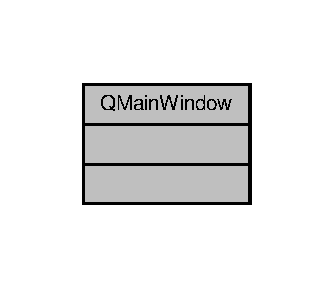
\includegraphics[width=160pt]{class_q_main_window__coll__graph}
\end{center}
\end{figure}


La documentation de cette classe a été générée à partir du fichier suivant \+:\begin{DoxyCompactItemize}
\item 
\hyperlink{_i_h_m_afficheur_8h}{I\+H\+M\+Afficheur.\+h}\end{DoxyCompactItemize}

\hypertarget{class_q_object}{}\subsection{Référence de la classe Q\+Object}
\label{class_q_object}\index{Q\+Object@{Q\+Object}}


Graphe de collaboration de Q\+Object\+:
\nopagebreak
\begin{figure}[H]
\begin{center}
\leavevmode
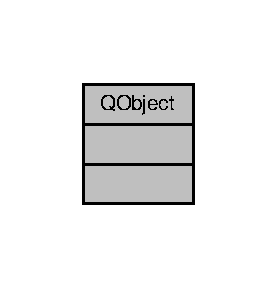
\includegraphics[width=133pt]{class_q_object__coll__graph}
\end{center}
\end{figure}


La documentation de cette classe a été générée à partir du fichier suivant \+:\begin{DoxyCompactItemize}
\item 
\hyperlink{_rencontre_8h}{Rencontre.\+h}\end{DoxyCompactItemize}

\hypertarget{class_rencontre}{}\subsection{Référence de la classe Rencontre}
\label{class_rencontre}\index{Rencontre@{Rencontre}}


{\ttfamily \#include $<$Rencontre.\+h$>$}



Graphe de collaboration de Rencontre\+:
\nopagebreak
\begin{figure}[H]
\begin{center}
\leavevmode
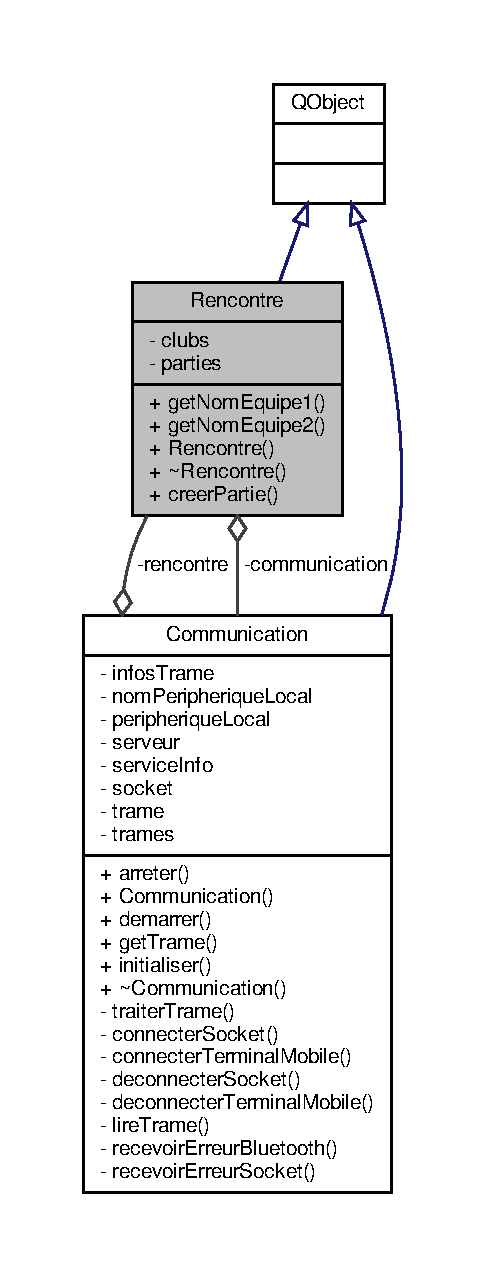
\includegraphics[height=550pt]{class_rencontre__coll__graph}
\end{center}
\end{figure}
\subsubsection*{Connecteurs publics}
\begin{DoxyCompactItemize}
\item 
void \hyperlink{class_rencontre_a8eb8eb61ed543925626e7680a1ecef5b}{creer\+Partie} (Q\+String\+List info\+Trame)
\end{DoxyCompactItemize}
\subsubsection*{Fonctions membres publiques}
\begin{DoxyCompactItemize}
\item 
Q\+String \hyperlink{class_rencontre_a50df24caf57437d8eaaadae43ff846ec}{get\+Nom\+Equipe1} ()
\item 
Q\+String \hyperlink{class_rencontre_ac544f97755480e0e2718d0802d308585}{get\+Nom\+Equipe2} ()
\item 
\hyperlink{class_rencontre_aab1bbf3ea211e00186ab7f866994b77a}{Rencontre} (Q\+String nom\+Club1=\char`\"{}nom\+Club1\char`\"{}, Q\+String nom\+Club2=\char`\"{}nom\+Club1\char`\"{})
\item 
\hyperlink{class_rencontre_a437de7d5f9adced5124dcfdd13e504d3}{$\sim$\+Rencontre} ()
\end{DoxyCompactItemize}
\subsubsection*{Attributs privés}
\begin{DoxyCompactItemize}
\item 
Q\+Vector$<$ \hyperlink{class_club}{Club} $\ast$ $>$ \hyperlink{class_rencontre_a12f6cef62070ecb095971e704a9d92a6}{clubs}
\item 
\hyperlink{class_communication}{Communication} $\ast$ \hyperlink{class_rencontre_a843a1b93c1cb909f2706c6f81438661e}{communication}
\item 
Q\+Vector$<$ \hyperlink{class_partie}{Partie} $>$ \hyperlink{class_rencontre_a6b52ccf9b5d083718928b207ae5316fe}{parties}
\end{DoxyCompactItemize}


\subsubsection{Description détaillée}


Définition à la ligne \hyperlink{_rencontre_8h_source_l00025}{25} du fichier \hyperlink{_rencontre_8h_source}{Rencontre.\+h}.



\subsubsection{Documentation des constructeurs et destructeur}
\mbox{\Hypertarget{class_rencontre_aab1bbf3ea211e00186ab7f866994b77a}\label{class_rencontre_aab1bbf3ea211e00186ab7f866994b77a}} 
\index{Rencontre@{Rencontre}!Rencontre@{Rencontre}}
\index{Rencontre@{Rencontre}!Rencontre@{Rencontre}}
\paragraph{\texorpdfstring{Rencontre()}{Rencontre()}}
{\footnotesize\ttfamily Rencontre\+::\+Rencontre (\begin{DoxyParamCaption}\item[{Q\+String}]{nom\+Club1 = {\ttfamily \char`\"{}nomClub1\char`\"{}},  }\item[{Q\+String}]{nom\+Club2 = {\ttfamily \char`\"{}nomClub1\char`\"{}} }\end{DoxyParamCaption})}



Définition à la ligne \hyperlink{_rencontre_8cpp_source_l00015}{15} du fichier \hyperlink{_rencontre_8cpp_source}{Rencontre.\+cpp}.



Références \hyperlink{_rencontre_8h_source_l00030}{clubs}.


\begin{DoxyCode}
00016 \{
00017     qDebug() << Q\_FUNC\_INFO << nomClub1 << nomClub2;
00018     \hyperlink{class_rencontre_a12f6cef62070ecb095971e704a9d92a6}{clubs}.push\_back(\textcolor{keyword}{new} \hyperlink{class_club}{Club}(nomClub1));
00019     \hyperlink{class_rencontre_a12f6cef62070ecb095971e704a9d92a6}{clubs}.push\_back(\textcolor{keyword}{new} \hyperlink{class_club}{Club}(nomClub2));
00020 \}
\end{DoxyCode}
\mbox{\Hypertarget{class_rencontre_a437de7d5f9adced5124dcfdd13e504d3}\label{class_rencontre_a437de7d5f9adced5124dcfdd13e504d3}} 
\index{Rencontre@{Rencontre}!````~Rencontre@{$\sim$\+Rencontre}}
\index{````~Rencontre@{$\sim$\+Rencontre}!Rencontre@{Rencontre}}
\paragraph{\texorpdfstring{$\sim$\+Rencontre()}{~Rencontre()}}
{\footnotesize\ttfamily Rencontre\+::$\sim$\+Rencontre (\begin{DoxyParamCaption}{ }\end{DoxyParamCaption})}



Définition à la ligne \hyperlink{_rencontre_8cpp_source_l00022}{22} du fichier \hyperlink{_rencontre_8cpp_source}{Rencontre.\+cpp}.



Références \hyperlink{_rencontre_8h_source_l00030}{clubs}.


\begin{DoxyCode}
00023 \{
00024     \textcolor{keywordflow}{for}(\textcolor{keywordtype}{int} i=0; i<\hyperlink{class_rencontre_a12f6cef62070ecb095971e704a9d92a6}{clubs}.size(); i++)
00025     \{
00026         \textcolor{keyword}{delete} \hyperlink{class_rencontre_a12f6cef62070ecb095971e704a9d92a6}{clubs}[i];
00027     \}
00028     qDebug() << Q\_FUNC\_INFO;
00029 \}
\end{DoxyCode}


\subsubsection{Documentation des fonctions membres}
\mbox{\Hypertarget{class_rencontre_a8eb8eb61ed543925626e7680a1ecef5b}\label{class_rencontre_a8eb8eb61ed543925626e7680a1ecef5b}} 
\index{Rencontre@{Rencontre}!creer\+Partie@{creer\+Partie}}
\index{creer\+Partie@{creer\+Partie}!Rencontre@{Rencontre}}
\paragraph{\texorpdfstring{creer\+Partie}{creerPartie}}
{\footnotesize\ttfamily void Rencontre\+::creer\+Partie (\begin{DoxyParamCaption}\item[{Q\+String\+List}]{info\+Trame }\end{DoxyParamCaption})\hspace{0.3cm}{\ttfamily [slot]}}



Définition à la ligne \hyperlink{_rencontre_8cpp_source_l00031}{31} du fichier \hyperlink{_rencontre_8cpp_source}{Rencontre.\+cpp}.



Références \hyperlink{_rencontre_8h_source_l00031}{parties}.


\begin{DoxyCode}
00032 \{
00033     qDebug() << Q\_FUNC\_INFO;
00034     \hyperlink{class_rencontre_a6b52ccf9b5d083718928b207ae5316fe}{parties}.push\_back(\hyperlink{class_partie}{Partie}(\hyperlink{class_joueur}{Joueur}(infoTrame[3],infoTrame[4]), 
      \hyperlink{class_joueur}{Joueur}(infoTrame[5], infoTrame[6])));
00035 
00036 \textcolor{preprocessor}{    #ifdef DEBUG\_PARTIE}
00037     \hyperlink{class_rencontre_a6b52ccf9b5d083718928b207ae5316fe}{parties}[0].debugPartie();
00038 \textcolor{preprocessor}{    #endif}
00039 \}
\end{DoxyCode}
\mbox{\Hypertarget{class_rencontre_a50df24caf57437d8eaaadae43ff846ec}\label{class_rencontre_a50df24caf57437d8eaaadae43ff846ec}} 
\index{Rencontre@{Rencontre}!get\+Nom\+Equipe1@{get\+Nom\+Equipe1}}
\index{get\+Nom\+Equipe1@{get\+Nom\+Equipe1}!Rencontre@{Rencontre}}
\paragraph{\texorpdfstring{get\+Nom\+Equipe1()}{getNomEquipe1()}}
{\footnotesize\ttfamily Q\+String Rencontre\+::get\+Nom\+Equipe1 (\begin{DoxyParamCaption}{ }\end{DoxyParamCaption})}



Définition à la ligne \hyperlink{_rencontre_8cpp_source_l00041}{41} du fichier \hyperlink{_rencontre_8cpp_source}{Rencontre.\+cpp}.



Références \hyperlink{_rencontre_8h_source_l00030}{clubs}, et \hyperlink{_rencontre_8h_source_l00017}{E\+Q\+U\+I\+P\+E\+\_\+A}.



Référencé par \hyperlink{_i_h_m_afficheur_8cpp_source_l00100}{I\+H\+M\+Afficheur\+::afficher\+Rencontre()}, et \hyperlink{_i_h_m_afficheur_8cpp_source_l00090}{I\+H\+M\+Afficheur\+::commencer\+Rencontre()}.


\begin{DoxyCode}
00042 \{
00043     \textcolor{keywordflow}{if}(\hyperlink{class_rencontre_a12f6cef62070ecb095971e704a9d92a6}{clubs}.count() > 0)
00044         \textcolor{keywordflow}{return} \hyperlink{class_rencontre_a12f6cef62070ecb095971e704a9d92a6}{clubs}[\hyperlink{_rencontre_8h_ab4f4f1173fbbb2f1f27e2b18c5de79dc}{EQUIPE\_A}]->getNom();
00045     \textcolor{keywordflow}{else}
00046         \textcolor{keywordflow}{return} QString();
00047 \}
\end{DoxyCode}
\mbox{\Hypertarget{class_rencontre_ac544f97755480e0e2718d0802d308585}\label{class_rencontre_ac544f97755480e0e2718d0802d308585}} 
\index{Rencontre@{Rencontre}!get\+Nom\+Equipe2@{get\+Nom\+Equipe2}}
\index{get\+Nom\+Equipe2@{get\+Nom\+Equipe2}!Rencontre@{Rencontre}}
\paragraph{\texorpdfstring{get\+Nom\+Equipe2()}{getNomEquipe2()}}
{\footnotesize\ttfamily Q\+String Rencontre\+::get\+Nom\+Equipe2 (\begin{DoxyParamCaption}{ }\end{DoxyParamCaption})}



Définition à la ligne \hyperlink{_rencontre_8cpp_source_l00049}{49} du fichier \hyperlink{_rencontre_8cpp_source}{Rencontre.\+cpp}.



Références \hyperlink{_rencontre_8h_source_l00030}{clubs}, et \hyperlink{_rencontre_8h_source_l00018}{E\+Q\+U\+I\+P\+E\+\_\+X}.



Référencé par \hyperlink{_i_h_m_afficheur_8cpp_source_l00100}{I\+H\+M\+Afficheur\+::afficher\+Rencontre()}, et \hyperlink{_i_h_m_afficheur_8cpp_source_l00090}{I\+H\+M\+Afficheur\+::commencer\+Rencontre()}.


\begin{DoxyCode}
00050 \{
00051     \textcolor{keywordflow}{if}(\hyperlink{class_rencontre_a12f6cef62070ecb095971e704a9d92a6}{clubs}.count() > 0)
00052         \textcolor{keywordflow}{return} \hyperlink{class_rencontre_a12f6cef62070ecb095971e704a9d92a6}{clubs}[\hyperlink{_rencontre_8h_abee6bce8b9cc687177c72a76428afcff}{EQUIPE\_X}]->getNom();
00053     \textcolor{keywordflow}{else}
00054         \textcolor{keywordflow}{return} QString();
00055 \}
\end{DoxyCode}


\subsubsection{Documentation des données membres}
\mbox{\Hypertarget{class_rencontre_a12f6cef62070ecb095971e704a9d92a6}\label{class_rencontre_a12f6cef62070ecb095971e704a9d92a6}} 
\index{Rencontre@{Rencontre}!clubs@{clubs}}
\index{clubs@{clubs}!Rencontre@{Rencontre}}
\paragraph{\texorpdfstring{clubs}{clubs}}
{\footnotesize\ttfamily Q\+Vector$<$\hyperlink{class_club}{Club}$\ast$$>$ Rencontre\+::clubs\hspace{0.3cm}{\ttfamily [private]}}



Définition à la ligne \hyperlink{_rencontre_8h_source_l00030}{30} du fichier \hyperlink{_rencontre_8h_source}{Rencontre.\+h}.



Référencé par \hyperlink{_rencontre_8cpp_source_l00041}{get\+Nom\+Equipe1()}, \hyperlink{_rencontre_8cpp_source_l00049}{get\+Nom\+Equipe2()}, \hyperlink{_rencontre_8cpp_source_l00015}{Rencontre()}, et \hyperlink{_rencontre_8cpp_source_l00022}{$\sim$\+Rencontre()}.

\mbox{\Hypertarget{class_rencontre_a843a1b93c1cb909f2706c6f81438661e}\label{class_rencontre_a843a1b93c1cb909f2706c6f81438661e}} 
\index{Rencontre@{Rencontre}!communication@{communication}}
\index{communication@{communication}!Rencontre@{Rencontre}}
\paragraph{\texorpdfstring{communication}{communication}}
{\footnotesize\ttfamily \hyperlink{class_communication}{Communication}$\ast$ Rencontre\+::communication\hspace{0.3cm}{\ttfamily [private]}}



Définition à la ligne \hyperlink{_rencontre_8h_source_l00032}{32} du fichier \hyperlink{_rencontre_8h_source}{Rencontre.\+h}.

\mbox{\Hypertarget{class_rencontre_a6b52ccf9b5d083718928b207ae5316fe}\label{class_rencontre_a6b52ccf9b5d083718928b207ae5316fe}} 
\index{Rencontre@{Rencontre}!parties@{parties}}
\index{parties@{parties}!Rencontre@{Rencontre}}
\paragraph{\texorpdfstring{parties}{parties}}
{\footnotesize\ttfamily Q\+Vector$<$\hyperlink{class_partie}{Partie}$>$ Rencontre\+::parties\hspace{0.3cm}{\ttfamily [private]}}



Définition à la ligne \hyperlink{_rencontre_8h_source_l00031}{31} du fichier \hyperlink{_rencontre_8h_source}{Rencontre.\+h}.



Référencé par \hyperlink{_rencontre_8cpp_source_l00031}{creer\+Partie()}.



La documentation de cette classe a été générée à partir des fichiers suivants \+:\begin{DoxyCompactItemize}
\item 
\hyperlink{_rencontre_8h}{Rencontre.\+h}\item 
\hyperlink{_rencontre_8cpp}{Rencontre.\+cpp}\end{DoxyCompactItemize}

\section{Documentation des fichiers}
\hypertarget{_club_8cpp}{}\subsection{Référence du fichier Club.\+cpp}
\label{_club_8cpp}\index{Club.\+cpp@{Club.\+cpp}}


Définition de la classe \hyperlink{class_club}{Club}.  


{\ttfamily \#include \char`\"{}Club.\+h\char`\"{}}\newline
{\ttfamily \#include $<$Q\+Debug$>$}\newline


\subsubsection{Description détaillée}
Définition de la classe \hyperlink{class_club}{Club}. 

\begin{DoxyVersion}{Version}
1.\+0 
\end{DoxyVersion}
\begin{DoxyAuthor}{Auteur}
William G\+E\+R\+O\+U\+V\+I\+L\+LE \href{mailto:gerouwilliam@gmail.com}{\tt gerouwilliam@gmail.\+com} \$\+Last\+Changed\+Revision\$ \$\+Last\+Changed\+Date\$ 
\end{DoxyAuthor}


Définition dans le fichier \hyperlink{_club_8cpp_source}{Club.\+cpp}.


\hypertarget{_club_8cpp_source}{}\subsection{Club.\+cpp}

\begin{DoxyCode}
00001 \textcolor{preprocessor}{#include "\hyperlink{_club_8h}{Club.h}"}
00002 \textcolor{preprocessor}{#include <QDebug>}
00003 
\Hypertarget{_club_8cpp_source_l00013}\hyperlink{class_club_a6d6fa5971608a06394c40453289d6251}{00013} \hyperlink{class_club_a6d6fa5971608a06394c40453289d6251}{Club::Club}(QString nom) : nom(nom), partiesRemportees(0)
00014 \{
00015     qDebug() << Q\_FUNC\_INFO << nom << \textcolor{keyword}{this};
00016 \}
00017 
\Hypertarget{_club_8cpp_source_l00018}\hyperlink{class_club_a1c2993e141cfa6468284274359cc7de5}{00018} \hyperlink{class_club_a1c2993e141cfa6468284274359cc7de5}{Club::~Club}()
00019 \{
00020     qDebug() << Q\_FUNC\_INFO << \textcolor{keyword}{this};
00021 \}
00022 
\Hypertarget{_club_8cpp_source_l00023}\hyperlink{class_club_aaa3c96659bf305d7a1988ecbd27de30f}{00023} QString \hyperlink{class_club_aaa3c96659bf305d7a1988ecbd27de30f}{Club::getNom}()\textcolor{keyword}{ const}
00024 \textcolor{keyword}{}\{
00025     \textcolor{keywordflow}{return} this->\hyperlink{class_club_a18e1489d02110a82a0c8706f52091002}{nom};
00026 \}
00027 
\Hypertarget{_club_8cpp_source_l00028}\hyperlink{class_club_a6cb8e81d8cfd3d5febd6ce48e33ba94e}{00028} \textcolor{keywordtype}{void} \hyperlink{class_club_a6cb8e81d8cfd3d5febd6ce48e33ba94e}{Club::setNom}(QString &n)
00029 \{
00030     \hyperlink{class_club_a18e1489d02110a82a0c8706f52091002}{nom} = n;
00031 \}
00032 
\Hypertarget{_club_8cpp_source_l00033}\hyperlink{class_club_af4f28219aa51c3742cddfae4b66cec4b}{00033} \textcolor{keywordtype}{int} \hyperlink{class_club_af4f28219aa51c3742cddfae4b66cec4b}{Club::getPartiesRemportes}()\textcolor{keyword}{ const}
00034 \textcolor{keyword}{}\{
00035     \textcolor{keywordflow}{return} this->\hyperlink{class_club_a1c5dd1362656cb4829de483255ffc39a}{partiesRemportees};
00036 \}
00037 
\Hypertarget{_club_8cpp_source_l00038}\hyperlink{class_club_ad1711f2742e385ef00174b3ebd98b165}{00038} \textcolor{keywordtype}{void} \hyperlink{class_club_ad1711f2742e385ef00174b3ebd98b165}{Club::setPartiesRemportes}(\textcolor{keywordtype}{int} &p)
00039 \{
00040     \hyperlink{class_club_a1c5dd1362656cb4829de483255ffc39a}{partiesRemportees} = p;
00041 \}
00042 
\Hypertarget{_club_8cpp_source_l00043}\hyperlink{class_club_af7cf902fc29f6d587b11a10eec87edff}{00043} \textcolor{keywordtype}{void} \hyperlink{class_club_af7cf902fc29f6d587b11a10eec87edff}{Club::ajouterJoueur}(\textcolor{keywordtype}{char} &lettre, \hyperlink{class_joueur}{Joueur} &j)
00044 \{
00045     \hyperlink{class_club_a1546f281ba72a07e52cbfd2a60af699b}{joueurs}.insert(lettre,j);
00046 \}
\end{DoxyCode}

\hypertarget{_club_8h}{}\subsection{Référence du fichier Club.\+h}
\label{_club_8h}\index{Club.\+h@{Club.\+h}}


Déclaration de la classe \hyperlink{class_club}{Club}.  


{\ttfamily \#include $<$Q\+String$>$}\newline
{\ttfamily \#include $<$Q\+Map$>$}\newline
{\ttfamily \#include \char`\"{}Joueur.\+h\char`\"{}}\newline
\subsubsection*{Classes}
\begin{DoxyCompactItemize}
\item 
class \hyperlink{class_club}{Club}
\end{DoxyCompactItemize}


\subsubsection{Description détaillée}
Déclaration de la classe \hyperlink{class_club}{Club}. 

\begin{DoxyVersion}{Version}
1.\+0 
\end{DoxyVersion}
\begin{DoxyAuthor}{Auteur}
William G\+E\+R\+O\+U\+V\+I\+L\+LE \href{mailto:gerouwilliam@gmail.com}{\tt gerouwilliam@gmail.\+com} \$\+Last\+Changed\+Revision\$ \$\+Last\+Changed\+Date\$ 
\end{DoxyAuthor}


Définition dans le fichier \hyperlink{_club_8h_source}{Club.\+h}.


\hypertarget{_club_8h_source}{}\subsection{Club.\+h}

\begin{DoxyCode}
00001 \textcolor{preprocessor}{#ifndef CLUB\_H}
00002 \textcolor{preprocessor}{#define CLUB\_H}
00003 
00013 \textcolor{preprocessor}{#include <QString>}
00014 \textcolor{preprocessor}{#include <QMap>}
00015 \textcolor{preprocessor}{#include "\hyperlink{_joueur_8h}{Joueur.h}"}
00016 
\Hypertarget{_club_8h_source_l00017}\hyperlink{class_club}{00017} \textcolor{keyword}{class }\hyperlink{class_club}{Club}
00018 \{
00019 \textcolor{keyword}{private}:
\Hypertarget{_club_8h_source_l00020}\hyperlink{class_club_a18e1489d02110a82a0c8706f52091002}{00020}     QString \hyperlink{class_club_a18e1489d02110a82a0c8706f52091002}{nom};
\Hypertarget{_club_8h_source_l00021}\hyperlink{class_club_a1c5dd1362656cb4829de483255ffc39a}{00021}     \textcolor{keywordtype}{int} \hyperlink{class_club_a1c5dd1362656cb4829de483255ffc39a}{partiesRemportees};
\Hypertarget{_club_8h_source_l00022}\hyperlink{class_club_a1546f281ba72a07e52cbfd2a60af699b}{00022}     QMap<char,Joueur> \hyperlink{class_club_a1546f281ba72a07e52cbfd2a60af699b}{joueurs};
00023 
00024 \textcolor{keyword}{public}:
00025     \hyperlink{class_club_a6d6fa5971608a06394c40453289d6251}{Club}(QString nom = \textcolor{stringliteral}{""});
00026     \hyperlink{class_club_a1c2993e141cfa6468284274359cc7de5}{~Club}();
00027     QString \hyperlink{class_club_aaa3c96659bf305d7a1988ecbd27de30f}{getNom}()\textcolor{keyword}{const};
00028     \textcolor{keywordtype}{void} \hyperlink{class_club_a6cb8e81d8cfd3d5febd6ce48e33ba94e}{setNom}(QString &n);
00029     \textcolor{keywordtype}{int} \hyperlink{class_club_af4f28219aa51c3742cddfae4b66cec4b}{getPartiesRemportes}() \textcolor{keyword}{const};
00030     \textcolor{keywordtype}{void} \hyperlink{class_club_ad1711f2742e385ef00174b3ebd98b165}{setPartiesRemportes}(\textcolor{keywordtype}{int} &p);
00031     \textcolor{keywordtype}{void} \hyperlink{class_club_af7cf902fc29f6d587b11a10eec87edff}{ajouterJoueur}(\textcolor{keywordtype}{char} &lettre, \hyperlink{class_joueur}{Joueur} &j);
00032 \};
00033 
00034 \textcolor{preprocessor}{#endif // CLUB\_H}
\end{DoxyCode}

\hypertarget{_communication_8cpp}{}\subsection{Référence du fichier Communication.\+cpp}
\label{_communication_8cpp}\index{Communication.\+cpp@{Communication.\+cpp}}


Définition de la classe \hyperlink{class_communication}{Communication}.  


{\ttfamily \#include \char`\"{}Communication.\+h\char`\"{}}\newline
{\ttfamily \#include \char`\"{}Rencontre.\+h\char`\"{}}\newline
{\ttfamily \#include $<$Qt\+Debug$>$}\newline


\subsubsection{Description détaillée}
Définition de la classe \hyperlink{class_communication}{Communication}. 

\begin{DoxyVersion}{Version}
1.\+0 
\end{DoxyVersion}
\begin{DoxyAuthor}{Auteur}
William G\+E\+R\+O\+U\+V\+I\+L\+LE \href{mailto:gerouwilliam@gmail.com}{\tt gerouwilliam@gmail.\+com} \$\+Last\+Changed\+Revision\$ \$\+Last\+Changed\+Date\$ 
\end{DoxyAuthor}


Définition dans le fichier \hyperlink{_communication_8cpp_source}{Communication.\+cpp}.


\hypertarget{_communication_8cpp_source}{}\subsection{Communication.\+cpp}

\begin{DoxyCode}
00001 \textcolor{preprocessor}{#include "\hyperlink{_communication_8h}{Communication.h}"}
00002 \textcolor{preprocessor}{#include "\hyperlink{_rencontre_8h}{Rencontre.h}"}
00003 \textcolor{preprocessor}{#include <QtDebug>}
00004 
\Hypertarget{_communication_8cpp_source_l00020}\hyperlink{class_communication_a56cf4b262e592bcae1d987c3dd00487f}{00020} \hyperlink{class_communication_a56cf4b262e592bcae1d987c3dd00487f}{Communication::Communication}(\hyperlink{class_q_object}{QObject} *parent) : 
      \hyperlink{class_q_object}{QObject}(parent), serveur(nullptr), socket(nullptr)
00021 \{
00022     qDebug() << Q\_FUNC\_INFO;
00023 
00024     \hyperlink{class_communication_a2c10a52807bc7bdc520ec3fae622f672}{initialiser}();
00025 \}
00026 
\Hypertarget{_communication_8cpp_source_l00032}\hyperlink{class_communication_a75ba08ce908d45251e28e4c1db94e6f4}{00032} \hyperlink{class_communication_a75ba08ce908d45251e28e4c1db94e6f4}{Communication::~Communication}()
00033 \{
00034     qDebug() << Q\_FUNC\_INFO;
00035 
00036     \hyperlink{class_communication_a1f4b02441803f9c8e231cb9f304d776b}{arreter}();
00037 \}
00038 
\Hypertarget{_communication_8cpp_source_l00044}\hyperlink{class_communication_a2c10a52807bc7bdc520ec3fae622f672}{00044} \textcolor{keywordtype}{void} \hyperlink{class_communication_a2c10a52807bc7bdc520ec3fae622f672}{Communication::initialiser}()
00045 \{
00046     \textcolor{comment}{// vérifier la présence du Bluetooth}
00047     \textcolor{keywordflow}{if} (\hyperlink{class_communication_a2d643d199169dfe1d258df54d3ee5728}{peripheriqueLocal}.isValid())
00048     \{
00049         \textcolor{comment}{// activer le bluetooth}
00050         \hyperlink{class_communication_a2d643d199169dfe1d258df54d3ee5728}{peripheriqueLocal}.powerOn();
00051 
00052         \textcolor{comment}{// récupérer le nom du périphérique local}
00053         \hyperlink{class_communication_acfe0b2b569ebf174fcdd766272b89ba8}{nomPeripheriqueLocal} = \hyperlink{class_communication_a2d643d199169dfe1d258df54d3ee5728}{peripheriqueLocal}.name();
00054         qDebug() << Q\_FUNC\_INFO << \hyperlink{class_communication_acfe0b2b569ebf174fcdd766272b89ba8}{nomPeripheriqueLocal};
00055 
00056         \textcolor{comment}{// rendre le périphérique local découvrable et jumelable}
00057         \hyperlink{class_communication_a2d643d199169dfe1d258df54d3ee5728}{peripheriqueLocal}.setHostMode(QBluetoothLocalDevice::HostDiscoverable);
00058 
00059         \textcolor{comment}{// connecter les signaux et les slots}
00060         connect(&\hyperlink{class_communication_a2d643d199169dfe1d258df54d3ee5728}{peripheriqueLocal}, SIGNAL(deviceConnected(QBluetoothAddress)), \textcolor{keyword}{this}, SLOT
      (\hyperlink{class_communication_a9640339b93f4a99f80426b7345615037}{connecterTerminalMobile}(QBluetoothAddress)));
00061         connect(&\hyperlink{class_communication_a2d643d199169dfe1d258df54d3ee5728}{peripheriqueLocal}, SIGNAL(deviceDisconnected(QBluetoothAddress)), \textcolor{keyword}{this}, 
      SLOT(\hyperlink{class_communication_aeeb47bc3c4d7419fefb737168638442e}{deconnecterTerminalMobile}(QBluetoothAddress)));
00062         connect(&\hyperlink{class_communication_a2d643d199169dfe1d258df54d3ee5728}{peripheriqueLocal}, SIGNAL(error(QBluetoothLocalDevice::Error)), \textcolor{keyword}{this}, 
      SLOT(\hyperlink{class_communication_adbbab5630096d6374c4d7e52508b8a37}{recevoirErreurBluetooth}(QBluetoothLocalDevice::Error)));
00063     \}
00064     \textcolor{keywordflow}{else}
00065         qDebug() << Q\_FUNC\_INFO << \textcolor{stringliteral}{"Bluetooth non disponible !"};
00066 \}
00067 
\Hypertarget{_communication_8cpp_source_l00073}\hyperlink{class_communication_af29ea9a1c2ce29436f2331c322f6ebbf}{00073} \textcolor{keywordtype}{void} \hyperlink{class_communication_af29ea9a1c2ce29436f2331c322f6ebbf}{Communication::demarrer}()
00074 \{
00075     \textcolor{comment}{// vérifier la présence du Bluetooth}
00076     \textcolor{keywordflow}{if} (\hyperlink{class_communication_a2d643d199169dfe1d258df54d3ee5728}{peripheriqueLocal}.isValid() && \hyperlink{class_communication_a6384747297d6efa9e8fd2fc79ed0c269}{serveur} == \textcolor{keyword}{nullptr})
00077     \{
00078         \textcolor{comment}{// créer une socket serveur}
00079         \hyperlink{class_communication_a6384747297d6efa9e8fd2fc79ed0c269}{serveur} = \textcolor{keyword}{new} QBluetoothServer(QBluetoothServiceInfo::RfcommProtocol, \textcolor{keyword}{this});
00080 
00081         \textcolor{comment}{// connecter les signaux et les slots}
00082         connect(\hyperlink{class_communication_a6384747297d6efa9e8fd2fc79ed0c269}{serveur}, SIGNAL(newConnection()), \textcolor{keyword}{this}, SLOT(
      \hyperlink{class_communication_a1ef7e4107d98346290f19f76d7eecf32}{connecterSocket}()));
00083 
00084         \textcolor{comment}{// placer le serveur en écoute}
00085         QBluetoothUuid uuid = QBluetoothUuid(\hyperlink{_communication_8h_a6f285f3a7cee5c6573729d7e6b99dbf4}{uuidService});
00086         \hyperlink{class_communication_aa7f9ee5e5d90336a56857ebc229e4274}{serviceInfo} = \hyperlink{class_communication_a6384747297d6efa9e8fd2fc79ed0c269}{serveur}->listen(uuid, \hyperlink{_communication_8h_afd6061bebcd621de34bc921326538181}{nomService});
00087 
00088         qDebug() << Q\_FUNC\_INFO << \textcolor{stringliteral}{"Attente de connexion"};
00089     \}
00090     \textcolor{keywordflow}{else}
00091         qDebug() << Q\_FUNC\_INFO << \textcolor{stringliteral}{"Bluetooth non disponible !"};
00092 \}
00093 
\Hypertarget{_communication_8cpp_source_l00099}\hyperlink{class_communication_a1f4b02441803f9c8e231cb9f304d776b}{00099} \textcolor{keywordtype}{void} \hyperlink{class_communication_a1f4b02441803f9c8e231cb9f304d776b}{Communication::arreter}()
00100 \{    
00101     \textcolor{keywordflow}{if} (\hyperlink{class_communication_a6384747297d6efa9e8fd2fc79ed0c269}{serveur} == \textcolor{keyword}{nullptr})
00102         \textcolor{keywordflow}{return};
00103 
00104     \textcolor{keywordflow}{if} (\hyperlink{class_communication_aa4ddc3151b305db0135d5826384645cc}{socket} != \textcolor{keyword}{nullptr})
00105     \{
00106         \hyperlink{class_communication_a5280c11bea5ead32e7a7101fd5b0f9b2}{deconnecterSocket}();
00107     \}
00108 
00109     \textcolor{keyword}{delete} \hyperlink{class_communication_a6384747297d6efa9e8fd2fc79ed0c269}{serveur};
00110     \hyperlink{class_communication_a6384747297d6efa9e8fd2fc79ed0c269}{serveur} = \textcolor{keyword}{nullptr};
00111     qDebug() << Q\_FUNC\_INFO;
00112 
00113     \hyperlink{class_communication_a2d643d199169dfe1d258df54d3ee5728}{peripheriqueLocal}.setHostMode(QBluetoothLocalDevice::HostPoweredOff);
00114 \}
00115 
\Hypertarget{_communication_8cpp_source_l00116}\hyperlink{class_communication_a1ef7e4107d98346290f19f76d7eecf32}{00116} \textcolor{keywordtype}{void} \hyperlink{class_communication_a1ef7e4107d98346290f19f76d7eecf32}{Communication::connecterSocket}()
00117 \{
00118     \hyperlink{class_communication_aa4ddc3151b305db0135d5826384645cc}{socket} = \hyperlink{class_communication_a6384747297d6efa9e8fd2fc79ed0c269}{serveur}->nextPendingConnection();
00119     \textcolor{keywordflow}{if} (!\hyperlink{class_communication_aa4ddc3151b305db0135d5826384645cc}{socket})
00120         \textcolor{keywordflow}{return};
00121 
00122     qDebug() << Q\_FUNC\_INFO;
00123     \hyperlink{class_communication_aa4ddc3151b305db0135d5826384645cc}{socket}->open(QIODevice::ReadOnly);
00124     connect(\hyperlink{class_communication_aa4ddc3151b305db0135d5826384645cc}{socket}, SIGNAL(readyRead()), \textcolor{keyword}{this}, SLOT(\hyperlink{class_communication_ad99afe857470e6e95432b3adcb97fea2}{lireTrame}()));
00125     connect(\hyperlink{class_communication_aa4ddc3151b305db0135d5826384645cc}{socket}, SIGNAL(disconnected()), \textcolor{keyword}{this}, SLOT(\hyperlink{class_communication_a5280c11bea5ead32e7a7101fd5b0f9b2}{deconnecterSocket}()));
00126     connect(\hyperlink{class_communication_aa4ddc3151b305db0135d5826384645cc}{socket}, SIGNAL(error(QBluetoothSocket::SocketError)), \textcolor{keyword}{this}, SLOT(
      \hyperlink{class_communication_a94a9c34e683d590fc6abbc4111a57f29}{recevoirErreurSocket}(QBluetoothSocket::SocketError)));
00127 
00131 \}
00132 
\Hypertarget{_communication_8cpp_source_l00133}\hyperlink{class_communication_a5280c11bea5ead32e7a7101fd5b0f9b2}{00133} \textcolor{keywordtype}{void} \hyperlink{class_communication_a5280c11bea5ead32e7a7101fd5b0f9b2}{Communication::deconnecterSocket}()
00134 \{    
00135     \textcolor{keywordflow}{if} (\hyperlink{class_communication_aa4ddc3151b305db0135d5826384645cc}{socket}->isOpen())
00136        \hyperlink{class_communication_aa4ddc3151b305db0135d5826384645cc}{socket}->close();
00137     \textcolor{keyword}{delete} \hyperlink{class_communication_aa4ddc3151b305db0135d5826384645cc}{socket};
00138     \hyperlink{class_communication_aa4ddc3151b305db0135d5826384645cc}{socket} = \textcolor{keyword}{nullptr};
00139     qDebug() << Q\_FUNC\_INFO;
00140 \}
00141 
\Hypertarget{_communication_8cpp_source_l00142}\hyperlink{class_communication_a94a9c34e683d590fc6abbc4111a57f29}{00142} \textcolor{keywordtype}{void} \hyperlink{class_communication_a94a9c34e683d590fc6abbc4111a57f29}{Communication::recevoirErreurSocket}(QBluetoothSocket::SocketError e
      )
00143 \{
00144     qDebug() << Q\_FUNC\_INFO << e;
00145 \}
00146 
\Hypertarget{_communication_8cpp_source_l00147}\hyperlink{class_communication_a9640339b93f4a99f80426b7345615037}{00147} \textcolor{keywordtype}{void} \hyperlink{class_communication_a9640339b93f4a99f80426b7345615037}{Communication::connecterTerminalMobile}(\textcolor{keyword}{const} QBluetoothAddress &
      adresse)
00148 \{
00149     \textcolor{keywordflow}{if} (\hyperlink{class_communication_a2d643d199169dfe1d258df54d3ee5728}{peripheriqueLocal}.pairingStatus(adresse) == QBluetoothLocalDevice::Paired || 
      \hyperlink{class_communication_a2d643d199169dfe1d258df54d3ee5728}{peripheriqueLocal}.pairingStatus(adresse) == QBluetoothLocalDevice::AuthorizedPaired)
00150     \{
00151         qDebug() << Q\_FUNC\_INFO << adresse.toString() << \textcolor{stringliteral}{"appairé"};
00155     \}
00156     \textcolor{keywordflow}{else}
00157         qDebug() << Q\_FUNC\_INFO << adresse.toString() << \textcolor{stringliteral}{"non appairé"};
00158 \}
00159 
\Hypertarget{_communication_8cpp_source_l00160}\hyperlink{class_communication_aeeb47bc3c4d7419fefb737168638442e}{00160} \textcolor{keywordtype}{void} \hyperlink{class_communication_aeeb47bc3c4d7419fefb737168638442e}{Communication::deconnecterTerminalMobile}(\textcolor{keyword}{const} 
      QBluetoothAddress &adresse)
00161 \{
00162     qDebug() << Q\_FUNC\_INFO << adresse;
00166 \}
00167 
\Hypertarget{_communication_8cpp_source_l00168}\hyperlink{class_communication_adbbab5630096d6374c4d7e52508b8a37}{00168} \textcolor{keywordtype}{void} \hyperlink{class_communication_adbbab5630096d6374c4d7e52508b8a37}{Communication::recevoirErreurBluetooth}(
      QBluetoothLocalDevice::Error erreurBluetooth)
00169 \{
00170     qDebug() << Q\_FUNC\_INFO << erreurBluetooth;
00171 \}
00172 
\Hypertarget{_communication_8cpp_source_l00173}\hyperlink{class_communication_ad99afe857470e6e95432b3adcb97fea2}{00173} \textcolor{keywordtype}{void} \hyperlink{class_communication_ad99afe857470e6e95432b3adcb97fea2}{Communication::lireTrame}()
00174 \{
00175     QByteArray donnees;
00176 
00177     \textcolor{comment}{// lit les données reçues}
00178     donnees = \hyperlink{class_communication_aa4ddc3151b305db0135d5826384645cc}{socket}->readAll();
00179     qDebug() << Q\_FUNC\_INFO << donnees;
00180 
00181     \textcolor{comment}{// ajoute les données reçues}
00182     \hyperlink{class_communication_ac8f5004bfaaf7f538ba5ae93255f772b}{trame} += QString(donnees.data());
00183     qDebug() << Q\_FUNC\_INFO << \hyperlink{class_communication_ac8f5004bfaaf7f538ba5ae93255f772b}{trame};
00184 
00185     \textcolor{comment}{// au moins une trame complète reçue ?}
00186     \textcolor{keywordflow}{if}(trame.startsWith(\hyperlink{_communication_8h_a226742d7ade287673fb2295df90f462b}{ENTETE\_TRAME}) && trame.endsWith(\textcolor{stringliteral}{"\(\backslash\)r\(\backslash\)n"}))
00187     \{
00188         \textcolor{comment}{// si plusieurs trames reçues}
00189         QStringList \hyperlink{class_communication_a89b75dc8f2d3427478660b45c01f4186}{trames} = trame.split(\textcolor{stringliteral}{"\(\backslash\)r\(\backslash\)n"}, QString::SkipEmptyParts);
00190         qDebug() << Q\_FUNC\_INFO << \hyperlink{class_communication_a89b75dc8f2d3427478660b45c01f4186}{trames};
00191 
00192         \textcolor{comment}{// traite les trames reçues}
00193         \textcolor{keywordflow}{for}(\textcolor{keywordtype}{int} i = 0; i < trames.count(); ++i)
00194         \{
00195             qDebug() << Q\_FUNC\_INFO << i << trames[i];
00196 
00197             \textcolor{comment}{// découpe les champs de la trame}
00198             \hyperlink{class_communication_a219fe9a4cd04470241f26f1f6159d721}{infosTrame} = trames[i].split(\textcolor{stringliteral}{";"});
00199 
00200             \hyperlink{class_communication_a1f17fd8330b55b3ab30263d15e6e740b}{traiterTrame}(\hyperlink{class_communication_a219fe9a4cd04470241f26f1f6159d721}{infosTrame});
00201         \}
00202 
00203         \textcolor{comment}{// reinitialise trame pour la prochaine réception}
00204         trame.clear();
00205     \}
00206 \}
00207 
\Hypertarget{_communication_8cpp_source_l00208}\hyperlink{class_communication_a1f17fd8330b55b3ab30263d15e6e740b}{00208} \textcolor{keywordtype}{bool} \hyperlink{class_communication_a1f17fd8330b55b3ab30263d15e6e740b}{Communication::traiterTrame}(QStringList 
      \hyperlink{class_communication_a219fe9a4cd04470241f26f1f6159d721}{infosTrame})
00209 \{
00210     \textcolor{keywordflow}{if}(infosTrame.count() < \hyperlink{_communication_8h_a2aab79787b26ad74e8cb5ab837236791}{CHAMP\_TYPE\_TRAME})
00211         \textcolor{keywordflow}{return} \textcolor{keyword}{false};
00212 
00213     qDebug() << Q\_FUNC\_INFO << \hyperlink{class_communication_a219fe9a4cd04470241f26f1f6159d721}{infosTrame};
00214 
00215     \textcolor{keywordflow}{switch}(infosTrame[\hyperlink{_communication_8h_a2aab79787b26ad74e8cb5ab837236791}{CHAMP\_TYPE\_TRAME}].toInt())
00216     \{
00220         \textcolor{keywordflow}{case} \hyperlink{_communication_8h_ad794b2a211d6c4ead603d7ebd097a992af8ce6111c15264884121829746e18a1f}{TypeTrame::RENCONTRE}:
00221             emit(\hyperlink{class_communication_af3430c844d728e4ec3961744243324e1}{debutRencontre}(infosTrame[2], infosTrame[3]));
00222             \textcolor{keywordflow}{break};
00223 
00224         \textcolor{keywordflow}{case} \hyperlink{_communication_8h_ad794b2a211d6c4ead603d7ebd097a992ac3a2021df6ca4ad18f8af3ce95931122}{TypeTrame::INFO\_PARTIE}:
00225             emit(\hyperlink{class_communication_a3d8a1dccee9867e6b84932ddc3072b45}{creationPartie}(infosTrame));
00226             \textcolor{keywordflow}{break};
00227 
00228         \textcolor{keywordflow}{case} \hyperlink{_communication_8h_ad794b2a211d6c4ead603d7ebd097a992af57444a2814db96222f09035ff269767}{TypeTrame::SCORE}:
00229             emit(\hyperlink{class_communication_acf4446d47652e0c508296e52df6fb11b}{nouveauScorePartie}());
00230             \textcolor{keywordflow}{break};
00231 
00232         \textcolor{keywordflow}{case} \hyperlink{_communication_8h_ad794b2a211d6c4ead603d7ebd097a992a6f91d1f6dd2600af9ca6a66ffe2adba2}{TypeTrame::ETAT\_PARTIE}:
00233             emit(\hyperlink{class_communication_af5444d470230a6e817ca8bc9484eb169}{changementEtatPartie}());
00234             \textcolor{keywordflow}{break};
00235 
00236         \textcolor{keywordflow}{case} \hyperlink{_communication_8h_ad794b2a211d6c4ead603d7ebd097a992a09c331e69591a2470471d457a17b413c}{TypeTrame::NET}:
00237             emit(\hyperlink{class_communication_a4c828450e0ff92818c878ee28f240662}{detectionNET}());
00238             \textcolor{keywordflow}{break};
00239 
00240         \textcolor{keywordflow}{case} \hyperlink{_communication_8h_ad794b2a211d6c4ead603d7ebd097a992a2f4a926417575653ebbe1ca64a16974f}{TypeTrame::TEMPS\_MORT}:
00241             emit(\hyperlink{class_communication_ab2dd9f10ceaba18016017104683b6fc1}{demandeTempsMort}());
00242             \textcolor{keywordflow}{break};
00243 
00244         \textcolor{keywordflow}{default}:
00245             qDebug() << Q\_FUNC\_INFO << \textcolor{stringliteral}{"Type de trame inconnu !"};
00246             \textcolor{keywordflow}{return} \textcolor{keyword}{false};
00247     \}
00248 
00249     \textcolor{keywordflow}{return} \textcolor{keyword}{true};
00250 \}
00251 
\Hypertarget{_communication_8cpp_source_l00252}\hyperlink{class_communication_ad8dbd75b168bc02c76306361e650bbba}{00252} QString \hyperlink{class_communication_ad8dbd75b168bc02c76306361e650bbba}{Communication::getTrame}()\textcolor{keyword}{ const}
00253 \textcolor{keyword}{}\{
00254     \textcolor{keywordflow}{return} \hyperlink{class_communication_ac8f5004bfaaf7f538ba5ae93255f772b}{trame};
00255 \}
\end{DoxyCode}

\hypertarget{_communication_8h}{}\subsection{Référence du fichier Communication.\+h}
\label{_communication_8h}\index{Communication.\+h@{Communication.\+h}}


Déclaration de la classe \hyperlink{class_communication}{Communication}.  


{\ttfamily \#include $<$Q\+Object$>$}\newline
{\ttfamily \#include $<$Q\+String$>$}\newline
{\ttfamily \#include $<$Q\+Bluetooth\+Local\+Device$>$}\newline
{\ttfamily \#include $<$Q\+Bluetooth\+Server$>$}\newline
{\ttfamily \#include $<$Q\+Bluetooth\+Socket$>$}\newline
\subsubsection*{Classes}
\begin{DoxyCompactItemize}
\item 
class \hyperlink{class_communication}{Communication}
\begin{DoxyCompactList}\small\item\em Déclaration de la classe \hyperlink{class_communication}{Communication}. \end{DoxyCompactList}\end{DoxyCompactItemize}
\subsubsection*{Macros}
\begin{DoxyCompactItemize}
\item 
\#define \hyperlink{_communication_8h_a2aab79787b26ad74e8cb5ab837236791}{C\+H\+A\+M\+P\+\_\+\+T\+Y\+P\+E\+\_\+\+T\+R\+A\+ME}~1
\item 
\#define \hyperlink{_communication_8h_a226742d7ade287673fb2295df90f462b}{E\+N\+T\+E\+T\+E\+\_\+\+T\+R\+A\+ME}~\char`\"{}M\+O\+B\+I\+L\+E\+\_\+\+A\+R\+EA\char`\"{}
\end{DoxyCompactItemize}
\subsubsection*{Énumérations}
\begin{DoxyCompactItemize}
\item 
enum \hyperlink{_communication_8h_ad794b2a211d6c4ead603d7ebd097a992}{Type\+Trame} \{ \newline
\hyperlink{_communication_8h_ad794b2a211d6c4ead603d7ebd097a992af8ce6111c15264884121829746e18a1f}{R\+E\+N\+C\+O\+N\+T\+RE}, 
\hyperlink{_communication_8h_ad794b2a211d6c4ead603d7ebd097a992ac3a2021df6ca4ad18f8af3ce95931122}{I\+N\+F\+O\+\_\+\+P\+A\+R\+T\+IE}, 
\hyperlink{_communication_8h_ad794b2a211d6c4ead603d7ebd097a992af57444a2814db96222f09035ff269767}{S\+C\+O\+RE}, 
\hyperlink{_communication_8h_ad794b2a211d6c4ead603d7ebd097a992a6f91d1f6dd2600af9ca6a66ffe2adba2}{E\+T\+A\+T\+\_\+\+P\+A\+R\+T\+IE}, 
\newline
\hyperlink{_communication_8h_ad794b2a211d6c4ead603d7ebd097a992a09c331e69591a2470471d457a17b413c}{N\+ET}, 
\hyperlink{_communication_8h_ad794b2a211d6c4ead603d7ebd097a992a2f4a926417575653ebbe1ca64a16974f}{T\+E\+M\+P\+S\+\_\+\+M\+O\+RT}
 \}\begin{DoxyCompactList}\small\item\em Les différents types de trame. \end{DoxyCompactList}
\end{DoxyCompactItemize}
\subsubsection*{Fonctions}
\begin{DoxyCompactItemize}
\item 
static const Q\+String \hyperlink{_communication_8h_afd6061bebcd621de34bc921326538181}{nom\+Service} (Q\+String\+Literal(\char`\"{}Afficheur\+\_\+\+A\+R\+EA\char`\"{}))
\item 
static const Q\+String \hyperlink{_communication_8h_a6f285f3a7cee5c6573729d7e6b99dbf4}{uuid\+Service} (Q\+String\+Literal(\char`\"{}0000110a-\/0000-\/1000-\/8000-\/00805f9b34fb\char`\"{}))
\end{DoxyCompactItemize}


\subsubsection{Description détaillée}
Déclaration de la classe \hyperlink{class_communication}{Communication}. 

\begin{DoxyVersion}{Version}
1.\+0 
\end{DoxyVersion}
\begin{DoxyAuthor}{Auteur}
William G\+E\+R\+O\+U\+V\+I\+L\+LE \href{mailto:gerouwilliam@gmail.com}{\tt gerouwilliam@gmail.\+com} \$\+Last\+Changed\+Revision\$ \$\+Last\+Changed\+Date\$ 
\end{DoxyAuthor}


Définition dans le fichier \hyperlink{_communication_8h_source}{Communication.\+h}.



\subsubsection{Documentation des macros}
\mbox{\Hypertarget{_communication_8h_a2aab79787b26ad74e8cb5ab837236791}\label{_communication_8h_a2aab79787b26ad74e8cb5ab837236791}} 
\index{Communication.\+h@{Communication.\+h}!C\+H\+A\+M\+P\+\_\+\+T\+Y\+P\+E\+\_\+\+T\+R\+A\+ME@{C\+H\+A\+M\+P\+\_\+\+T\+Y\+P\+E\+\_\+\+T\+R\+A\+ME}}
\index{C\+H\+A\+M\+P\+\_\+\+T\+Y\+P\+E\+\_\+\+T\+R\+A\+ME@{C\+H\+A\+M\+P\+\_\+\+T\+Y\+P\+E\+\_\+\+T\+R\+A\+ME}!Communication.\+h@{Communication.\+h}}
\paragraph{\texorpdfstring{C\+H\+A\+M\+P\+\_\+\+T\+Y\+P\+E\+\_\+\+T\+R\+A\+ME}{CHAMP\_TYPE\_TRAME}}
{\footnotesize\ttfamily \#define C\+H\+A\+M\+P\+\_\+\+T\+Y\+P\+E\+\_\+\+T\+R\+A\+ME~1}



Définition à la ligne \hyperlink{_communication_8h_source_l00020}{20} du fichier \hyperlink{_communication_8h_source}{Communication.\+h}.



Référencé par \hyperlink{_communication_8cpp_source_l00208}{Communication\+::traiter\+Trame()}.

\mbox{\Hypertarget{_communication_8h_a226742d7ade287673fb2295df90f462b}\label{_communication_8h_a226742d7ade287673fb2295df90f462b}} 
\index{Communication.\+h@{Communication.\+h}!E\+N\+T\+E\+T\+E\+\_\+\+T\+R\+A\+ME@{E\+N\+T\+E\+T\+E\+\_\+\+T\+R\+A\+ME}}
\index{E\+N\+T\+E\+T\+E\+\_\+\+T\+R\+A\+ME@{E\+N\+T\+E\+T\+E\+\_\+\+T\+R\+A\+ME}!Communication.\+h@{Communication.\+h}}
\paragraph{\texorpdfstring{E\+N\+T\+E\+T\+E\+\_\+\+T\+R\+A\+ME}{ENTETE\_TRAME}}
{\footnotesize\ttfamily \#define E\+N\+T\+E\+T\+E\+\_\+\+T\+R\+A\+ME~\char`\"{}M\+O\+B\+I\+L\+E\+\_\+\+A\+R\+EA\char`\"{}}



Définition à la ligne \hyperlink{_communication_8h_source_l00019}{19} du fichier \hyperlink{_communication_8h_source}{Communication.\+h}.



Référencé par \hyperlink{_communication_8cpp_source_l00173}{Communication\+::lire\+Trame()}.



\subsubsection{Documentation du type de l\textquotesingle{}énumération}
\mbox{\Hypertarget{_communication_8h_ad794b2a211d6c4ead603d7ebd097a992}\label{_communication_8h_ad794b2a211d6c4ead603d7ebd097a992}} 
\index{Communication.\+h@{Communication.\+h}!Type\+Trame@{Type\+Trame}}
\index{Type\+Trame@{Type\+Trame}!Communication.\+h@{Communication.\+h}}
\paragraph{\texorpdfstring{Type\+Trame}{TypeTrame}}
{\footnotesize\ttfamily enum \hyperlink{_communication_8h_ad794b2a211d6c4ead603d7ebd097a992}{Type\+Trame}}



Les différents types de trame. 

\begin{DoxyEnumFields}{Valeurs énumérées}
\raisebox{\heightof{T}}[0pt][0pt]{\index{R\+E\+N\+C\+O\+N\+T\+RE@{R\+E\+N\+C\+O\+N\+T\+RE}!Communication.\+h@{Communication.\+h}}\index{Communication.\+h@{Communication.\+h}!R\+E\+N\+C\+O\+N\+T\+RE@{R\+E\+N\+C\+O\+N\+T\+RE}}}\mbox{\Hypertarget{_communication_8h_ad794b2a211d6c4ead603d7ebd097a992af8ce6111c15264884121829746e18a1f}\label{_communication_8h_ad794b2a211d6c4ead603d7ebd097a992af8ce6111c15264884121829746e18a1f}} 
R\+E\+N\+C\+O\+N\+T\+RE&... \\
\hline

\raisebox{\heightof{T}}[0pt][0pt]{\index{I\+N\+F\+O\+\_\+\+P\+A\+R\+T\+IE@{I\+N\+F\+O\+\_\+\+P\+A\+R\+T\+IE}!Communication.\+h@{Communication.\+h}}\index{Communication.\+h@{Communication.\+h}!I\+N\+F\+O\+\_\+\+P\+A\+R\+T\+IE@{I\+N\+F\+O\+\_\+\+P\+A\+R\+T\+IE}}}\mbox{\Hypertarget{_communication_8h_ad794b2a211d6c4ead603d7ebd097a992ac3a2021df6ca4ad18f8af3ce95931122}\label{_communication_8h_ad794b2a211d6c4ead603d7ebd097a992ac3a2021df6ca4ad18f8af3ce95931122}} 
I\+N\+F\+O\+\_\+\+P\+A\+R\+T\+IE&\\
\hline

\raisebox{\heightof{T}}[0pt][0pt]{\index{S\+C\+O\+RE@{S\+C\+O\+RE}!Communication.\+h@{Communication.\+h}}\index{Communication.\+h@{Communication.\+h}!S\+C\+O\+RE@{S\+C\+O\+RE}}}\mbox{\Hypertarget{_communication_8h_ad794b2a211d6c4ead603d7ebd097a992af57444a2814db96222f09035ff269767}\label{_communication_8h_ad794b2a211d6c4ead603d7ebd097a992af57444a2814db96222f09035ff269767}} 
S\+C\+O\+RE&\\
\hline

\raisebox{\heightof{T}}[0pt][0pt]{\index{E\+T\+A\+T\+\_\+\+P\+A\+R\+T\+IE@{E\+T\+A\+T\+\_\+\+P\+A\+R\+T\+IE}!Communication.\+h@{Communication.\+h}}\index{Communication.\+h@{Communication.\+h}!E\+T\+A\+T\+\_\+\+P\+A\+R\+T\+IE@{E\+T\+A\+T\+\_\+\+P\+A\+R\+T\+IE}}}\mbox{\Hypertarget{_communication_8h_ad794b2a211d6c4ead603d7ebd097a992a6f91d1f6dd2600af9ca6a66ffe2adba2}\label{_communication_8h_ad794b2a211d6c4ead603d7ebd097a992a6f91d1f6dd2600af9ca6a66ffe2adba2}} 
E\+T\+A\+T\+\_\+\+P\+A\+R\+T\+IE&\\
\hline

\raisebox{\heightof{T}}[0pt][0pt]{\index{N\+ET@{N\+ET}!Communication.\+h@{Communication.\+h}}\index{Communication.\+h@{Communication.\+h}!N\+ET@{N\+ET}}}\mbox{\Hypertarget{_communication_8h_ad794b2a211d6c4ead603d7ebd097a992a09c331e69591a2470471d457a17b413c}\label{_communication_8h_ad794b2a211d6c4ead603d7ebd097a992a09c331e69591a2470471d457a17b413c}} 
N\+ET&\\
\hline

\raisebox{\heightof{T}}[0pt][0pt]{\index{T\+E\+M\+P\+S\+\_\+\+M\+O\+RT@{T\+E\+M\+P\+S\+\_\+\+M\+O\+RT}!Communication.\+h@{Communication.\+h}}\index{Communication.\+h@{Communication.\+h}!T\+E\+M\+P\+S\+\_\+\+M\+O\+RT@{T\+E\+M\+P\+S\+\_\+\+M\+O\+RT}}}\mbox{\Hypertarget{_communication_8h_ad794b2a211d6c4ead603d7ebd097a992a2f4a926417575653ebbe1ca64a16974f}\label{_communication_8h_ad794b2a211d6c4ead603d7ebd097a992a2f4a926417575653ebbe1ca64a16974f}} 
T\+E\+M\+P\+S\+\_\+\+M\+O\+RT&\\
\hline

\end{DoxyEnumFields}


Définition à la ligne \hyperlink{_communication_8h_source_l00026}{26} du fichier \hyperlink{_communication_8h_source}{Communication.\+h}.


\begin{DoxyCode}
00027 \{
00028     \hyperlink{_communication_8h_ad794b2a211d6c4ead603d7ebd097a992af8ce6111c15264884121829746e18a1f}{RENCONTRE}, 
00029     \hyperlink{_communication_8h_ad794b2a211d6c4ead603d7ebd097a992ac3a2021df6ca4ad18f8af3ce95931122}{INFO\_PARTIE},
00030     \hyperlink{_communication_8h_ad794b2a211d6c4ead603d7ebd097a992af57444a2814db96222f09035ff269767}{SCORE},
00031     \hyperlink{_communication_8h_ad794b2a211d6c4ead603d7ebd097a992a6f91d1f6dd2600af9ca6a66ffe2adba2}{ETAT\_PARTIE},
00032     \hyperlink{_communication_8h_ad794b2a211d6c4ead603d7ebd097a992a09c331e69591a2470471d457a17b413c}{NET},
00033     \hyperlink{_communication_8h_ad794b2a211d6c4ead603d7ebd097a992a2f4a926417575653ebbe1ca64a16974f}{TEMPS\_MORT},
00034 \};
\end{DoxyCode}


\subsubsection{Documentation des fonctions}
\mbox{\Hypertarget{_communication_8h_afd6061bebcd621de34bc921326538181}\label{_communication_8h_afd6061bebcd621de34bc921326538181}} 
\index{Communication.\+h@{Communication.\+h}!nom\+Service@{nom\+Service}}
\index{nom\+Service@{nom\+Service}!Communication.\+h@{Communication.\+h}}
\paragraph{\texorpdfstring{nom\+Service()}{nomService()}}
{\footnotesize\ttfamily static const Q\+String nom\+Service (\begin{DoxyParamCaption}\item[{Q\+String\+Literal(\char`\"{}Afficheur\+\_\+\+A\+R\+EA\char`\"{})}]{ }\end{DoxyParamCaption})\hspace{0.3cm}{\ttfamily [static]}}



Référencé par \hyperlink{_communication_8cpp_source_l00073}{Communication\+::demarrer()}.

\mbox{\Hypertarget{_communication_8h_a6f285f3a7cee5c6573729d7e6b99dbf4}\label{_communication_8h_a6f285f3a7cee5c6573729d7e6b99dbf4}} 
\index{Communication.\+h@{Communication.\+h}!uuid\+Service@{uuid\+Service}}
\index{uuid\+Service@{uuid\+Service}!Communication.\+h@{Communication.\+h}}
\paragraph{\texorpdfstring{uuid\+Service()}{uuidService()}}
{\footnotesize\ttfamily static const Q\+String uuid\+Service (\begin{DoxyParamCaption}\item[{Q\+String\+Literal(\char`\"{}0000110a-\/0000-\/1000-\/8000-\/00805f9b34fb\char`\"{})}]{ }\end{DoxyParamCaption})\hspace{0.3cm}{\ttfamily [static]}}



Référencé par \hyperlink{_communication_8cpp_source_l00073}{Communication\+::demarrer()}.


\hypertarget{_communication_8h_source}{}\subsection{Communication.\+h}

\begin{DoxyCode}
00001 \textcolor{preprocessor}{#ifndef COMMUNICATION\_H}
00002 \textcolor{preprocessor}{#define COMMUNICATION\_H}
00003 
00004 \textcolor{preprocessor}{#include <QObject>}
00005 \textcolor{preprocessor}{#include <QString>}
00006 \textcolor{preprocessor}{#include <QBluetoothLocalDevice>}
00007 \textcolor{preprocessor}{#include <QBluetoothServer>}
00008 \textcolor{preprocessor}{#include <QBluetoothSocket>}
00009 
\Hypertarget{_communication_8h_source_l00019}\hyperlink{_communication_8h_a226742d7ade287673fb2295df90f462b}{00019} \textcolor{preprocessor}{#define ENTETE\_TRAME        "MOBILE\_AREA"}
\Hypertarget{_communication_8h_source_l00020}\hyperlink{_communication_8h_a2aab79787b26ad74e8cb5ab837236791}{00020} \textcolor{preprocessor}{#define CHAMP\_TYPE\_TRAME    1}
00021 
\Hypertarget{_communication_8h_source_l00026}\hyperlink{_communication_8h_ad794b2a211d6c4ead603d7ebd097a992}{00026} \textcolor{keyword}{enum} \hyperlink{_communication_8h_ad794b2a211d6c4ead603d7ebd097a992}{TypeTrame}
00027 \{
\Hypertarget{_communication_8h_source_l00028}\hyperlink{_communication_8h_ad794b2a211d6c4ead603d7ebd097a992af8ce6111c15264884121829746e18a1f}{00028}     \hyperlink{_communication_8h_ad794b2a211d6c4ead603d7ebd097a992af8ce6111c15264884121829746e18a1f}{RENCONTRE}, 
\Hypertarget{_communication_8h_source_l00029}\hyperlink{_communication_8h_ad794b2a211d6c4ead603d7ebd097a992ac3a2021df6ca4ad18f8af3ce95931122}{00029}     \hyperlink{_communication_8h_ad794b2a211d6c4ead603d7ebd097a992ac3a2021df6ca4ad18f8af3ce95931122}{INFO\_PARTIE},
\Hypertarget{_communication_8h_source_l00030}\hyperlink{_communication_8h_ad794b2a211d6c4ead603d7ebd097a992af57444a2814db96222f09035ff269767}{00030}     \hyperlink{_communication_8h_ad794b2a211d6c4ead603d7ebd097a992af57444a2814db96222f09035ff269767}{SCORE},
\Hypertarget{_communication_8h_source_l00031}\hyperlink{_communication_8h_ad794b2a211d6c4ead603d7ebd097a992a6f91d1f6dd2600af9ca6a66ffe2adba2}{00031}     \hyperlink{_communication_8h_ad794b2a211d6c4ead603d7ebd097a992a6f91d1f6dd2600af9ca6a66ffe2adba2}{ETAT\_PARTIE},
\Hypertarget{_communication_8h_source_l00032}\hyperlink{_communication_8h_ad794b2a211d6c4ead603d7ebd097a992a09c331e69591a2470471d457a17b413c}{00032}     \hyperlink{_communication_8h_ad794b2a211d6c4ead603d7ebd097a992a09c331e69591a2470471d457a17b413c}{NET},
\Hypertarget{_communication_8h_source_l00033}\hyperlink{_communication_8h_ad794b2a211d6c4ead603d7ebd097a992a2f4a926417575653ebbe1ca64a16974f}{00033}     \hyperlink{_communication_8h_ad794b2a211d6c4ead603d7ebd097a992a2f4a926417575653ebbe1ca64a16974f}{TEMPS\_MORT},
00034 \};
00035 
00036 \textcolor{keyword}{static} \textcolor{keyword}{const} QString \hyperlink{_communication_8h_a6f285f3a7cee5c6573729d7e6b99dbf4}{uuidService}(QStringLiteral(\textcolor{stringliteral}{"0000110a-0000-1000-8000-00805f9b34fb"}));
00037 \textcolor{keyword}{static} \textcolor{keyword}{const} QString \hyperlink{_communication_8h_afd6061bebcd621de34bc921326538181}{nomService}(QStringLiteral(\textcolor{stringliteral}{"Afficheur\_AREA"}));
00038 
00039 \textcolor{keyword}{class }\hyperlink{class_rencontre}{Rencontre};
00040 
\Hypertarget{_communication_8h_source_l00046}\hyperlink{class_communication}{00046} \textcolor{keyword}{class }\hyperlink{class_communication}{Communication} : \textcolor{keyword}{public} \hyperlink{class_q_object}{QObject}
00047 \{
00048     Q\_OBJECT
00049 \textcolor{keyword}{private}:
\Hypertarget{_communication_8h_source_l00050}\hyperlink{class_communication_acb471e5da168acc149c5e4e90d8b601c}{00050}     \hyperlink{class_rencontre}{Rencontre} *\hyperlink{class_communication_acb471e5da168acc149c5e4e90d8b601c}{rencontre};
\Hypertarget{_communication_8h_source_l00051}\hyperlink{class_communication_a6384747297d6efa9e8fd2fc79ed0c269}{00051}     QBluetoothServer *\hyperlink{class_communication_a6384747297d6efa9e8fd2fc79ed0c269}{serveur};                  
\Hypertarget{_communication_8h_source_l00052}\hyperlink{class_communication_aa4ddc3151b305db0135d5826384645cc}{00052}     QBluetoothSocket *\hyperlink{class_communication_aa4ddc3151b305db0135d5826384645cc}{socket};                   
\Hypertarget{_communication_8h_source_l00053}\hyperlink{class_communication_a2d643d199169dfe1d258df54d3ee5728}{00053}     QBluetoothLocalDevice \hyperlink{class_communication_a2d643d199169dfe1d258df54d3ee5728}{peripheriqueLocal};    
\Hypertarget{_communication_8h_source_l00054}\hyperlink{class_communication_aa7f9ee5e5d90336a56857ebc229e4274}{00054}     QBluetoothServiceInfo \hyperlink{class_communication_aa7f9ee5e5d90336a56857ebc229e4274}{serviceInfo};          
\Hypertarget{_communication_8h_source_l00055}\hyperlink{class_communication_acfe0b2b569ebf174fcdd766272b89ba8}{00055}     QString \hyperlink{class_communication_acfe0b2b569ebf174fcdd766272b89ba8}{nomPeripheriqueLocal};               
\Hypertarget{_communication_8h_source_l00056}\hyperlink{class_communication_ac8f5004bfaaf7f538ba5ae93255f772b}{00056}     QString \hyperlink{class_communication_ac8f5004bfaaf7f538ba5ae93255f772b}{trame};                              
\Hypertarget{_communication_8h_source_l00057}\hyperlink{class_communication_a89b75dc8f2d3427478660b45c01f4186}{00057}     QString \hyperlink{class_communication_a89b75dc8f2d3427478660b45c01f4186}{trames};                             
\Hypertarget{_communication_8h_source_l00058}\hyperlink{class_communication_a219fe9a4cd04470241f26f1f6159d721}{00058}     QStringList \hyperlink{class_communication_a219fe9a4cd04470241f26f1f6159d721}{infosTrame};                     
00059 
00060     \textcolor{keywordtype}{bool} \hyperlink{class_communication_a1f17fd8330b55b3ab30263d15e6e740b}{traiterTrame}(QStringList infosTrame);
00061 
00062 \textcolor{keyword}{public}:
00063     \hyperlink{class_communication_a56cf4b262e592bcae1d987c3dd00487f}{Communication}(\hyperlink{class_q_object}{QObject} *parent = \textcolor{keyword}{nullptr});
00064     \hyperlink{class_communication_a75ba08ce908d45251e28e4c1db94e6f4}{~Communication}();
00065 
00066     \textcolor{keywordtype}{void} \hyperlink{class_communication_a2c10a52807bc7bdc520ec3fae622f672}{initialiser}();                         
00067     \textcolor{keywordtype}{void} \hyperlink{class_communication_af29ea9a1c2ce29436f2331c322f6ebbf}{demarrer}();                            
00068     \textcolor{keywordtype}{void} \hyperlink{class_communication_a1f4b02441803f9c8e231cb9f304d776b}{arreter}();                             
00069     QString \hyperlink{class_communication_ad8dbd75b168bc02c76306361e650bbba}{getTrame}() \textcolor{keyword}{const};                   \textcolor{comment}{// ???}
00070 
00071 \textcolor{keyword}{private} slots:
00072     \textcolor{keywordtype}{void} \hyperlink{class_communication_a1ef7e4107d98346290f19f76d7eecf32}{connecterSocket}();
00073     \textcolor{keywordtype}{void} \hyperlink{class_communication_a5280c11bea5ead32e7a7101fd5b0f9b2}{deconnecterSocket}();
00074     \textcolor{keywordtype}{void} \hyperlink{class_communication_a94a9c34e683d590fc6abbc4111a57f29}{recevoirErreurSocket}(QBluetoothSocket::SocketError e);
00075     \textcolor{keywordtype}{void} \hyperlink{class_communication_a9640339b93f4a99f80426b7345615037}{connecterTerminalMobile}(\textcolor{keyword}{const} QBluetoothAddress &adresse);
00076     \textcolor{keywordtype}{void} \hyperlink{class_communication_aeeb47bc3c4d7419fefb737168638442e}{deconnecterTerminalMobile}(\textcolor{keyword}{const} QBluetoothAddress &adresse);
00077     \textcolor{keywordtype}{void} \hyperlink{class_communication_adbbab5630096d6374c4d7e52508b8a37}{recevoirErreurBluetooth}(QBluetoothLocalDevice::Error erreurBluetooth);
00078     \textcolor{keywordtype}{void} \hyperlink{class_communication_ad99afe857470e6e95432b3adcb97fea2}{lireTrame}();
00079 
00080 signals:
00081     \textcolor{keywordtype}{void} \hyperlink{class_communication_af3430c844d728e4ec3961744243324e1}{debutRencontre}(QString club1, QString club2);
00082     \textcolor{keywordtype}{void} \hyperlink{class_communication_a3d8a1dccee9867e6b84932ddc3072b45}{creationPartie}(QStringList infoTrame);
00083     \textcolor{keywordtype}{void} \hyperlink{class_communication_acf4446d47652e0c508296e52df6fb11b}{nouveauScorePartie}();
00084     \textcolor{keywordtype}{void} \hyperlink{class_communication_af5444d470230a6e817ca8bc9484eb169}{changementEtatPartie}();
00085     \textcolor{keywordtype}{void} \hyperlink{class_communication_a4c828450e0ff92818c878ee28f240662}{detectionNET}();
00086     \textcolor{keywordtype}{void} \hyperlink{class_communication_ab2dd9f10ceaba18016017104683b6fc1}{demandeTempsMort}();
00087 \};
00088 
00089 \textcolor{preprocessor}{#endif // COMMUNICATION\_H}
\end{DoxyCode}

\hypertarget{_i_h_m_afficheur_8cpp}{}\subsection{Référence du fichier I\+H\+M\+Afficheur.\+cpp}
\label{_i_h_m_afficheur_8cpp}\index{I\+H\+M\+Afficheur.\+cpp@{I\+H\+M\+Afficheur.\+cpp}}


Définition de la classe \hyperlink{class_i_h_m_afficheur}{I\+H\+M\+Afficheur}.  


{\ttfamily \#include \char`\"{}I\+H\+M\+Afficheur.\+h\char`\"{}}\newline
{\ttfamily \#include \char`\"{}ui\+\_\+\+I\+H\+M\+Afficheur.\+h\char`\"{}}\newline
{\ttfamily \#include \char`\"{}Rencontre.\+h\char`\"{}}\newline
{\ttfamily \#include \char`\"{}Communication.\+h\char`\"{}}\newline
{\ttfamily \#include $<$Qt\+Debug$>$}\newline


\subsubsection{Description détaillée}
Définition de la classe \hyperlink{class_i_h_m_afficheur}{I\+H\+M\+Afficheur}. 

\begin{DoxyVersion}{Version}
1.\+0 
\end{DoxyVersion}
\begin{DoxyAuthor}{Auteur}
William G\+E\+R\+O\+U\+V\+I\+L\+LE \href{mailto:gerouwilliam@gmail.com}{\tt gerouwilliam@gmail.\+com} \$\+Last\+Changed\+Revision\$ \$\+Last\+Changed\+Date\$ 
\end{DoxyAuthor}


Définition dans le fichier \hyperlink{_i_h_m_afficheur_8cpp_source}{I\+H\+M\+Afficheur.\+cpp}.


\hypertarget{_i_h_m_afficheur_8cpp_source}{}\subsection{I\+H\+M\+Afficheur.\+cpp}

\begin{DoxyCode}
00001 \textcolor{preprocessor}{#include "\hyperlink{_i_h_m_afficheur_8h}{IHMAfficheur.h}"}
00002 \textcolor{preprocessor}{#include "ui\_IHMAfficheur.h"}
00003 \textcolor{preprocessor}{#include "\hyperlink{_rencontre_8h}{Rencontre.h}"}
00004 \textcolor{preprocessor}{#include "\hyperlink{_communication_8h}{Communication.h}"}
00005 \textcolor{preprocessor}{#include <QtDebug>}
00006 
\Hypertarget{_i_h_m_afficheur_8cpp_source_l00022}\hyperlink{class_i_h_m_afficheur_a2fdf6626a1d9c2c635110a6e6ab703f9}{00022} \hyperlink{class_i_h_m_afficheur_a2fdf6626a1d9c2c635110a6e6ab703f9}{IHMAfficheur::IHMAfficheur}(QWidget *parent) : 
      \hyperlink{class_q_main_window}{QMainWindow}(parent), ui(new \hyperlink{namespace_ui}{Ui}::\hyperlink{class_i_h_m_afficheur}{IHMAfficheur}), rencontre(nullptr), communication(
      nullptr)
00023 \{
00024     qDebug() << Q\_FUNC\_INFO;
00025 
00026     \hyperlink{class_i_h_m_afficheur_a119539fa51bf2e091e77faedf82eb146}{initialiserIHM}();
00027 
00028 \textcolor{preprocessor}{    #ifndef TEST\_SANS\_BLUETOOTH}
00029     \hyperlink{class_i_h_m_afficheur_ab7a8db8e7cfa6dc86ab59a07ede75298}{initialiserCommunication}();
00030 \textcolor{preprocessor}{    #endif}
00031 
00032 \textcolor{preprocessor}{    #ifdef TEST\_SANS\_BLUETOOTH}
00033     \hyperlink{class_i_h_m_afficheur_ad2dc0742d9cdda731a16c570fd6f2434}{commencerRencontre}(\textcolor{stringliteral}{"Avignon"}, \textcolor{stringliteral}{"Orange"});
00034 \textcolor{preprocessor}{    #endif}
00035 \}
00036 
\Hypertarget{_i_h_m_afficheur_8cpp_source_l00043}\hyperlink{class_i_h_m_afficheur_aba47ddf68f3966ed8f5c697b48e352a4}{00043} \hyperlink{class_i_h_m_afficheur_aba47ddf68f3966ed8f5c697b48e352a4}{IHMAfficheur::~IHMAfficheur}()
00044 \{
00045     \textcolor{keywordflow}{if}(\hyperlink{class_i_h_m_afficheur_aef34d340f7ea30f049a98efc47bd9779}{rencontre} != \textcolor{keyword}{nullptr})
00046         \textcolor{keyword}{delete} \hyperlink{class_i_h_m_afficheur_aef34d340f7ea30f049a98efc47bd9779}{rencontre};
00047     \textcolor{keyword}{delete} \hyperlink{class_i_h_m_afficheur_a26ca43f1ff87b1caa2191adcce444d23}{ui};
00048     qDebug() << Q\_FUNC\_INFO;
00049 \}
00050 
\Hypertarget{_i_h_m_afficheur_8cpp_source_l00056}\hyperlink{class_i_h_m_afficheur_a119539fa51bf2e091e77faedf82eb146}{00056} \textcolor{keywordtype}{void} \hyperlink{class_i_h_m_afficheur_a119539fa51bf2e091e77faedf82eb146}{IHMAfficheur::initialiserIHM}()
00057 \{
00058     \hyperlink{class_i_h_m_afficheur_a26ca43f1ff87b1caa2191adcce444d23}{ui}->setupUi(\textcolor{keyword}{this});
00059 
00060     \hyperlink{class_i_h_m_afficheur_a26ca43f1ff87b1caa2191adcce444d23}{ui}->centralWidget->setStyleSheet(\textcolor{stringliteral}{"QWidget#centralWidget \{background-color: black;\} QLabel \{color:
       white\}"});
00061 
00062     \textcolor{comment}{// Mode debug}
00063     QAction *quitter = \textcolor{keyword}{new} QAction(\textcolor{keyword}{this});
00064     quitter->setShortcut(QKeySequence(QKeySequence(Qt::Key\_Escape)));
00065     addAction(quitter);
00066     connect(quitter, SIGNAL(triggered()), \textcolor{keyword}{this}, SLOT(close()));
00067 \}
00068 
\Hypertarget{_i_h_m_afficheur_8cpp_source_l00074}\hyperlink{class_i_h_m_afficheur_ab7a8db8e7cfa6dc86ab59a07ede75298}{00074} \textcolor{keywordtype}{void} \hyperlink{class_i_h_m_afficheur_ab7a8db8e7cfa6dc86ab59a07ede75298}{IHMAfficheur::initialiserCommunication}()
00075 \{
00076     \hyperlink{class_i_h_m_afficheur_a331b5544e96cc908336a1486b52c379b}{communication} = \textcolor{keyword}{new} \hyperlink{class_communication}{Communication}(\textcolor{keyword}{this});
00077 
00078     connect(\hyperlink{class_i_h_m_afficheur_a331b5544e96cc908336a1486b52c379b}{communication}, SIGNAL(debutRencontre(QString,QString)), \textcolor{keyword}{this}, SLOT(
      \hyperlink{class_i_h_m_afficheur_ad2dc0742d9cdda731a16c570fd6f2434}{commencerRencontre}(QString,QString)));
00079 
00080     \hyperlink{class_i_h_m_afficheur_a331b5544e96cc908336a1486b52c379b}{communication}->\hyperlink{class_communication_af29ea9a1c2ce29436f2331c322f6ebbf}{demarrer}();
00081 \}
00082 
\Hypertarget{_i_h_m_afficheur_8cpp_source_l00090}\hyperlink{class_i_h_m_afficheur_ad2dc0742d9cdda731a16c570fd6f2434}{00090} \textcolor{keywordtype}{void} \hyperlink{class_i_h_m_afficheur_ad2dc0742d9cdda731a16c570fd6f2434}{IHMAfficheur::commencerRencontre}(QString club1, QString club2)
00091 \{
00092     \hyperlink{class_i_h_m_afficheur_aef34d340f7ea30f049a98efc47bd9779}{rencontre} = \textcolor{keyword}{new} \hyperlink{class_rencontre}{Rencontre}(club1, club2);
00093     qDebug() << Q\_FUNC\_INFO << \hyperlink{class_i_h_m_afficheur_aef34d340f7ea30f049a98efc47bd9779}{rencontre}->\hyperlink{class_rencontre_a50df24caf57437d8eaaadae43ff846ec}{getNomEquipe1}() << \textcolor{stringliteral}{"vs"} << 
      \hyperlink{class_i_h_m_afficheur_aef34d340f7ea30f049a98efc47bd9779}{rencontre}->\hyperlink{class_rencontre_ac544f97755480e0e2718d0802d308585}{getNomEquipe2}();
00094 
00095     \hyperlink{class_i_h_m_afficheur_aec1fee14a130ea53206bf5f8e532b819}{afficherRencontre}();
00096 
00097     connect(\hyperlink{class_i_h_m_afficheur_a331b5544e96cc908336a1486b52c379b}{communication}, SIGNAL(creationPartie(QStringList)), 
      \hyperlink{class_i_h_m_afficheur_aef34d340f7ea30f049a98efc47bd9779}{rencontre}, SLOT(creerPartie(QStringList)));
00098 \}
00099 
\Hypertarget{_i_h_m_afficheur_8cpp_source_l00100}\hyperlink{class_i_h_m_afficheur_aec1fee14a130ea53206bf5f8e532b819}{00100} \textcolor{keywordtype}{void} \hyperlink{class_i_h_m_afficheur_aec1fee14a130ea53206bf5f8e532b819}{IHMAfficheur::afficherRencontre}()
00101 \{
00102     \hyperlink{class_i_h_m_afficheur_a26ca43f1ff87b1caa2191adcce444d23}{ui}->nomEquipe1->setText(\hyperlink{class_i_h_m_afficheur_aef34d340f7ea30f049a98efc47bd9779}{rencontre}->\hyperlink{class_rencontre_a50df24caf57437d8eaaadae43ff846ec}{getNomEquipe1}());
00103     \hyperlink{class_i_h_m_afficheur_a26ca43f1ff87b1caa2191adcce444d23}{ui}->nomEquipe1->setAlignment(Qt::AlignCenter);
00104     \hyperlink{class_i_h_m_afficheur_a26ca43f1ff87b1caa2191adcce444d23}{ui}->nomEquipe2->setText(\hyperlink{class_i_h_m_afficheur_aef34d340f7ea30f049a98efc47bd9779}{rencontre}->\hyperlink{class_rencontre_ac544f97755480e0e2718d0802d308585}{getNomEquipe2}());
00105     \hyperlink{class_i_h_m_afficheur_a26ca43f1ff87b1caa2191adcce444d23}{ui}->nomEquipe2->setAlignment(Qt::AlignCenter);
00106 \}
\end{DoxyCode}

\hypertarget{_i_h_m_afficheur_8h}{}\subsection{Référence du fichier I\+H\+M\+Afficheur.\+h}
\label{_i_h_m_afficheur_8h}\index{I\+H\+M\+Afficheur.\+h@{I\+H\+M\+Afficheur.\+h}}


Déclaration de la classe \hyperlink{class_i_h_m_afficheur}{I\+H\+M\+Afficheur}.  


{\ttfamily \#include $<$Qt\+Widgets$>$}\newline
\subsubsection*{Classes}
\begin{DoxyCompactItemize}
\item 
class \hyperlink{class_i_h_m_afficheur}{I\+H\+M\+Afficheur}
\begin{DoxyCompactList}\small\item\em Déclaration de la classe \hyperlink{class_i_h_m_afficheur}{I\+H\+M\+Afficheur}. \end{DoxyCompactList}\end{DoxyCompactItemize}
\subsubsection*{Espaces de nommage}
\begin{DoxyCompactItemize}
\item 
 \hyperlink{namespace_ui}{Ui}
\end{DoxyCompactItemize}


\subsubsection{Description détaillée}
Déclaration de la classe \hyperlink{class_i_h_m_afficheur}{I\+H\+M\+Afficheur}. 

\begin{DoxyVersion}{Version}
1.\+0 
\end{DoxyVersion}
\begin{DoxyAuthor}{Auteur}
William G\+E\+R\+O\+U\+V\+I\+L\+LE \href{mailto:gerouwilliam@gmail.com}{\tt gerouwilliam@gmail.\+com} \$\+Last\+Changed\+Revision\$ \$\+Last\+Changed\+Date\$ 
\end{DoxyAuthor}


Définition dans le fichier \hyperlink{_i_h_m_afficheur_8h_source}{I\+H\+M\+Afficheur.\+h}.


\hypertarget{_i_h_m_afficheur_8h_source}{}\subsection{I\+H\+M\+Afficheur.\+h}

\begin{DoxyCode}
00001 \textcolor{preprocessor}{#ifndef IHMAFFICHEUR\_H}
00002 \textcolor{preprocessor}{#define IHMAFFICHEUR\_H}
00003 
00013 \textcolor{preprocessor}{#include <QtWidgets>}
00014 
00019 \textcolor{comment}{//#define TEST\_SANS\_BLUETOOTH}
00020 
00021 \textcolor{keyword}{class }\hyperlink{class_rencontre}{Rencontre};
00022 \textcolor{keyword}{class }\hyperlink{class_communication}{Communication};
00023 
\Hypertarget{_i_h_m_afficheur_8h_source_l00024}\hyperlink{namespace_ui}{00024} \textcolor{keyword}{namespace }\hyperlink{namespace_ui}{Ui}
00025 \{
00026     \textcolor{keyword}{class }\hyperlink{class_i_h_m_afficheur}{IHMAfficheur};
00027 \}
00028 
\Hypertarget{_i_h_m_afficheur_8h_source_l00034}\hyperlink{class_i_h_m_afficheur}{00034} \textcolor{keyword}{class }\hyperlink{class_i_h_m_afficheur}{IHMAfficheur} : \textcolor{keyword}{public} \hyperlink{class_q_main_window}{QMainWindow}
00035 \{
00036     Q\_OBJECT
00037 
00038 \textcolor{keyword}{private}:
\Hypertarget{_i_h_m_afficheur_8h_source_l00039}\hyperlink{class_i_h_m_afficheur_a26ca43f1ff87b1caa2191adcce444d23}{00039}     Ui::IHMAfficheur *\hyperlink{class_i_h_m_afficheur_a26ca43f1ff87b1caa2191adcce444d23}{ui};           
\Hypertarget{_i_h_m_afficheur_8h_source_l00040}\hyperlink{class_i_h_m_afficheur_aef34d340f7ea30f049a98efc47bd9779}{00040}     \hyperlink{class_rencontre}{Rencontre} *\hyperlink{class_i_h_m_afficheur_aef34d340f7ea30f049a98efc47bd9779}{rencontre};
\Hypertarget{_i_h_m_afficheur_8h_source_l00041}\hyperlink{class_i_h_m_afficheur_a331b5544e96cc908336a1486b52c379b}{00041}     \hyperlink{class_communication}{Communication} *\hyperlink{class_i_h_m_afficheur_a331b5544e96cc908336a1486b52c379b}{communication};
00042 
00043     \textcolor{keywordtype}{void} initialiserIHM();
00044     \textcolor{keywordtype}{void} initialiserCommunication();
00045     \textcolor{keywordtype}{void} afficherRencontre();
00046 
00047 \textcolor{keyword}{public}:
00048     \textcolor{keyword}{explicit} \hyperlink{class_i_h_m_afficheur}{IHMAfficheur}(QWidget *parent = 0);
00049     ~\hyperlink{class_i_h_m_afficheur}{IHMAfficheur}();
00050 
00051 \textcolor{keyword}{public} slots:
00052     \textcolor{keywordtype}{void} commencerRencontre(QString club1, QString club2);
00053 \};
00054 
00055 \textcolor{preprocessor}{#endif // IHMAFFICHEUR\_H}
\end{DoxyCode}

\hypertarget{_joueur_8cpp}{}\subsection{Référence du fichier Joueur.\+cpp}
\label{_joueur_8cpp}\index{Joueur.\+cpp@{Joueur.\+cpp}}


Définition de la classe \hyperlink{class_joueur}{Joueur}.  


{\ttfamily \#include \char`\"{}Joueur.\+h\char`\"{}}\newline
{\ttfamily \#include $<$Q\+Debug$>$}\newline


\subsubsection{Description détaillée}
Définition de la classe \hyperlink{class_joueur}{Joueur}. 

\begin{DoxyVersion}{Version}
1.\+0 
\end{DoxyVersion}
\begin{DoxyAuthor}{Auteur}
William G\+E\+R\+O\+U\+V\+I\+L\+LE \href{mailto:gerouwilliam@gmail.com}{\tt gerouwilliam@gmail.\+com} \$\+Last\+Changed\+Revision\$ \$\+Last\+Changed\+Date\$ 
\end{DoxyAuthor}


Définition dans le fichier \hyperlink{_joueur_8cpp_source}{Joueur.\+cpp}.


\hypertarget{_joueur_8cpp_source}{}\subsection{Joueur.\+cpp}

\begin{DoxyCode}
00001 \textcolor{preprocessor}{#include "\hyperlink{_joueur_8h}{Joueur.h}"}
00002 \textcolor{preprocessor}{#include <QDebug>}
00003 
\Hypertarget{_joueur_8cpp_source_l00013}\hyperlink{class_joueur_a75f73a73741b0faa59c75fc98b872765}{00013} \hyperlink{class_joueur_a75f73a73741b0faa59c75fc98b872765}{Joueur::Joueur}(QString nom, QString prenom) : nom(nom), prenom(prenom), estServeur(false), 
      echangesRemportes(0)
00014 \{
00015     qDebug() << Q\_FUNC\_INFO << nom << \hyperlink{class_joueur_a96d4237143c2e57b8025c4e116e95909}{prenom};
00016 \}
00017 
\Hypertarget{_joueur_8cpp_source_l00018}\hyperlink{class_joueur_a9fb594f755601ee77ce5884c4c0861f3}{00018} \hyperlink{class_joueur_a9fb594f755601ee77ce5884c4c0861f3}{Joueur::~Joueur}()
00019 \{
00020     qDebug() << Q\_FUNC\_INFO;
00021 \}
00022 
\Hypertarget{_joueur_8cpp_source_l00023}\hyperlink{class_joueur_a1d7082ab1f926eae1bd6834e901751a7}{00023} QString \hyperlink{class_joueur_a1d7082ab1f926eae1bd6834e901751a7}{Joueur::getNom}()\textcolor{keyword}{ const}
00024 \textcolor{keyword}{}\{
00025     \textcolor{keywordflow}{return} this->\hyperlink{class_joueur_ab06d7f1e6b482299bb03919e0cd2166d}{nom};
00026 \}
00027 
\Hypertarget{_joueur_8cpp_source_l00028}\hyperlink{class_joueur_a30fdb194cbf6d7c378d173cc133fc23e}{00028} \textcolor{keywordtype}{void} \hyperlink{class_joueur_a30fdb194cbf6d7c378d173cc133fc23e}{Joueur::setNom}(QString &n)
00029 \{
00030     \hyperlink{class_joueur_ab06d7f1e6b482299bb03919e0cd2166d}{nom} = n;
00031 \}
00032 
\Hypertarget{_joueur_8cpp_source_l00033}\hyperlink{class_joueur_ade527085b285ce86ea9e369bc9959032}{00033} QString \hyperlink{class_joueur_ade527085b285ce86ea9e369bc9959032}{Joueur::getPrenom}()\textcolor{keyword}{ const}
00034 \textcolor{keyword}{}\{
00035     \textcolor{keywordflow}{return} this->\hyperlink{class_joueur_a96d4237143c2e57b8025c4e116e95909}{prenom};
00036 \}
00037 
\Hypertarget{_joueur_8cpp_source_l00038}\hyperlink{class_joueur_a1425ea57a1f030a26d9beb1244e6caa2}{00038} \textcolor{keywordtype}{void} \hyperlink{class_joueur_a1425ea57a1f030a26d9beb1244e6caa2}{Joueur::setPrenom}(QString &p)
00039 \{
00040     \hyperlink{class_joueur_a96d4237143c2e57b8025c4e116e95909}{prenom} = p;
00041 \}
00042 
\Hypertarget{_joueur_8cpp_source_l00043}\hyperlink{class_joueur_a7bf0e45b6600ae3a68b4afdad6d884b7}{00043} \textcolor{keywordtype}{bool} \hyperlink{class_joueur_a7bf0e45b6600ae3a68b4afdad6d884b7}{Joueur::getEstServeur}()\textcolor{keyword}{ const}
00044 \textcolor{keyword}{}\{
00045     \textcolor{keywordflow}{return} this->\hyperlink{class_joueur_ac22161c9510ed38d6c65cdf6315737a5}{estServeur};
00046 \}
00047 
\Hypertarget{_joueur_8cpp_source_l00048}\hyperlink{class_joueur_aea42f5af160c61130d5252796378ad4f}{00048} \textcolor{keywordtype}{void} \hyperlink{class_joueur_aea42f5af160c61130d5252796378ad4f}{Joueur::setServeur}(\textcolor{keywordtype}{bool} &e)
00049 \{
00050     \hyperlink{class_joueur_ac22161c9510ed38d6c65cdf6315737a5}{estServeur} = e;
00051 \}
00052 
\Hypertarget{_joueur_8cpp_source_l00053}\hyperlink{class_joueur_affde221fc6d6bf633991fff4f11dd62b}{00053} \textcolor{keywordtype}{int} \hyperlink{class_joueur_affde221fc6d6bf633991fff4f11dd62b}{Joueur::getEchangesRemportes}()\textcolor{keyword}{ const}
00054 \textcolor{keyword}{}\{
00055     \textcolor{keywordflow}{return} \hyperlink{class_joueur_a23ab203e6bbfc1b2679a8457b99206dc}{echangesRemportes};
00056 \}
\end{DoxyCode}

\hypertarget{_joueur_8h}{}\subsection{Référence du fichier Joueur.\+h}
\label{_joueur_8h}\index{Joueur.\+h@{Joueur.\+h}}


Déclaration de la classe \hyperlink{class_joueur}{Joueur}.  


{\ttfamily \#include $<$Q\+String$>$}\newline
\subsubsection*{Classes}
\begin{DoxyCompactItemize}
\item 
class \hyperlink{class_joueur}{Joueur}
\end{DoxyCompactItemize}


\subsubsection{Description détaillée}
Déclaration de la classe \hyperlink{class_joueur}{Joueur}. 

\begin{DoxyVersion}{Version}
1.\+0 
\end{DoxyVersion}
\begin{DoxyAuthor}{Auteur}
William G\+E\+R\+O\+U\+V\+I\+L\+LE \href{mailto:gerouwilliam@gmail.com}{\tt gerouwilliam@gmail.\+com} \$\+Last\+Changed\+Revision\$ \$\+Last\+Changed\+Date\$ 
\end{DoxyAuthor}


Définition dans le fichier \hyperlink{_joueur_8h_source}{Joueur.\+h}.


\hypertarget{_joueur_8h_source}{}\subsection{Joueur.\+h}

\begin{DoxyCode}
00001 \textcolor{preprocessor}{#ifndef JOUEUR\_H}
00002 \textcolor{preprocessor}{#define JOUEUR\_H}
00003 
00013 \textcolor{preprocessor}{#include <QString>}
00014 
\Hypertarget{_joueur_8h_source_l00015}\hyperlink{class_joueur}{00015} \textcolor{keyword}{class }\hyperlink{class_joueur}{Joueur}
00016 \{
00017 \textcolor{keyword}{private}:
\Hypertarget{_joueur_8h_source_l00018}\hyperlink{class_joueur_ab06d7f1e6b482299bb03919e0cd2166d}{00018}     QString \hyperlink{class_joueur_ab06d7f1e6b482299bb03919e0cd2166d}{nom};
\Hypertarget{_joueur_8h_source_l00019}\hyperlink{class_joueur_a96d4237143c2e57b8025c4e116e95909}{00019}     QString \hyperlink{class_joueur_a96d4237143c2e57b8025c4e116e95909}{prenom};
\Hypertarget{_joueur_8h_source_l00020}\hyperlink{class_joueur_ac22161c9510ed38d6c65cdf6315737a5}{00020}     \textcolor{keywordtype}{bool} \hyperlink{class_joueur_ac22161c9510ed38d6c65cdf6315737a5}{estServeur};
\Hypertarget{_joueur_8h_source_l00021}\hyperlink{class_joueur_a23ab203e6bbfc1b2679a8457b99206dc}{00021}     \textcolor{keywordtype}{int} \hyperlink{class_joueur_a23ab203e6bbfc1b2679a8457b99206dc}{echangesRemportes};
00022 
00023 \textcolor{keyword}{public}:
00024     \hyperlink{class_joueur_a75f73a73741b0faa59c75fc98b872765}{Joueur}(QString nom =\textcolor{stringliteral}{"nomJoueur"}, QString prenom = \textcolor{stringliteral}{"PrenomJoueur"});
00025     \hyperlink{class_joueur_a9fb594f755601ee77ce5884c4c0861f3}{~Joueur}();
00026     QString \hyperlink{class_joueur_a1d7082ab1f926eae1bd6834e901751a7}{getNom}() \textcolor{keyword}{const};
00027     \textcolor{keywordtype}{void} \hyperlink{class_joueur_a30fdb194cbf6d7c378d173cc133fc23e}{setNom}(QString &n);
00028     QString \hyperlink{class_joueur_ade527085b285ce86ea9e369bc9959032}{getPrenom}() \textcolor{keyword}{const};
00029     \textcolor{keywordtype}{void} \hyperlink{class_joueur_a1425ea57a1f030a26d9beb1244e6caa2}{setPrenom}(QString &p);
00030     \textcolor{keywordtype}{bool} \hyperlink{class_joueur_a7bf0e45b6600ae3a68b4afdad6d884b7}{getEstServeur}() \textcolor{keyword}{const};
00031     \textcolor{keywordtype}{void} \hyperlink{class_joueur_aea42f5af160c61130d5252796378ad4f}{setServeur}(\textcolor{keywordtype}{bool} &e);
00032     \textcolor{keywordtype}{int} \hyperlink{class_joueur_affde221fc6d6bf633991fff4f11dd62b}{getEchangesRemportes}() \textcolor{keyword}{const};
00033 \};
00034 
00035 \textcolor{preprocessor}{#endif // JOUEUR\_H}
\end{DoxyCode}

\hypertarget{main_8cpp}{}\subsection{Référence du fichier main.\+cpp}
\label{main_8cpp}\index{main.\+cpp@{main.\+cpp}}


Programme principal A\+R\+EA.  


{\ttfamily \#include \char`\"{}I\+H\+M\+Afficheur.\+h\char`\"{}}\newline
{\ttfamily \#include $<$Q\+Application$>$}\newline
\subsubsection*{Fonctions}
\begin{DoxyCompactItemize}
\item 
int \hyperlink{main_8cpp_a0ddf1224851353fc92bfbff6f499fa97}{main} (int argc, char $\ast$argv\mbox{[}$\,$\mbox{]})
\end{DoxyCompactItemize}


\subsubsection{Description détaillée}
Programme principal A\+R\+EA. 

Crée et affiche en plein écran la fenêtre principale de l\textquotesingle{}application A\+R\+EA \begin{DoxyAuthor}{Auteur}
William G\+E\+R\+O\+U\+V\+I\+L\+LE \href{mailto:gerouwilliam@gmail.com}{\tt gerouwilliam@gmail.\+com} 
\end{DoxyAuthor}
\begin{DoxyVersion}{Version}
1.\+0
\end{DoxyVersion}

\begin{DoxyParams}{Paramètres}
{\em argc} & \\
\hline
{\em argv\mbox{[}$\,$\mbox{]}} & \\
\hline
\end{DoxyParams}
\begin{DoxyReturn}{Renvoie}
int \$\+Last\+Changed\+Revision\$ \$\+Last\+Changed\+Date\$ 
\end{DoxyReturn}


Définition dans le fichier \hyperlink{main_8cpp_source}{main.\+cpp}.



\subsubsection{Documentation des fonctions}
\mbox{\Hypertarget{main_8cpp_a0ddf1224851353fc92bfbff6f499fa97}\label{main_8cpp_a0ddf1224851353fc92bfbff6f499fa97}} 
\index{main.\+cpp@{main.\+cpp}!main@{main}}
\index{main@{main}!main.\+cpp@{main.\+cpp}}
\paragraph{\texorpdfstring{main()}{main()}}
{\footnotesize\ttfamily int main (\begin{DoxyParamCaption}\item[{int}]{argc,  }\item[{char $\ast$}]{argv\mbox{[}$\,$\mbox{]} }\end{DoxyParamCaption})}



Définition à la ligne \hyperlink{main_8cpp_source_l00019}{19} du fichier \hyperlink{main_8cpp_source}{main.\+cpp}.


\begin{DoxyCode}
00020 \{
00021     QApplication a(argc, argv);
00022     \hyperlink{class_i_h_m_afficheur}{IHMAfficheur} w;
00023 
00024     \textcolor{comment}{//w.show();}
00025     w.showFullScreen();
00026 
00027     \textcolor{keywordflow}{return} a.exec();
00028 \}
\end{DoxyCode}

\hypertarget{main_8cpp_source}{}\subsection{main.\+cpp}

\begin{DoxyCode}
00001 \textcolor{preprocessor}{#include "\hyperlink{_i_h_m_afficheur_8h}{IHMAfficheur.h}"}
00002 \textcolor{preprocessor}{#include <QApplication>}
00003 
\Hypertarget{main_8cpp_source_l00019}\hyperlink{main_8cpp_a0ddf1224851353fc92bfbff6f499fa97}{00019} \textcolor{keywordtype}{int} \hyperlink{main_8cpp_a0ddf1224851353fc92bfbff6f499fa97}{main}(\textcolor{keywordtype}{int} argc, \textcolor{keywordtype}{char} *argv[])
00020 \{
00021     QApplication a(argc, argv);
00022     \hyperlink{class_i_h_m_afficheur}{IHMAfficheur} w;
00023 
00024     \textcolor{comment}{//w.show();}
00025     w.showFullScreen();
00026 
00027     \textcolor{keywordflow}{return} a.exec();
00028 \}
\end{DoxyCode}

\hypertarget{_partie_8cpp}{}\subsection{Référence du fichier Partie.\+cpp}
\label{_partie_8cpp}\index{Partie.\+cpp@{Partie.\+cpp}}


Définition de la classe \hyperlink{class_partie}{Partie}.  


{\ttfamily \#include \char`\"{}Partie.\+h\char`\"{}}\newline
{\ttfamily \#include $<$Qt\+Debug$>$}\newline


\subsubsection{Description détaillée}
Définition de la classe \hyperlink{class_partie}{Partie}. 

\begin{DoxyVersion}{Version}
1.\+0 
\end{DoxyVersion}
\begin{DoxyAuthor}{Auteur}
William G\+E\+R\+O\+U\+V\+I\+L\+LE \href{mailto:gerouwilliam@gmail.com}{\tt gerouwilliam@gmail.\+com} \$\+Last\+Changed\+Revision\$ \$\+Last\+Changed\+Date\$ 
\end{DoxyAuthor}


Définition dans le fichier \hyperlink{_partie_8cpp_source}{Partie.\+cpp}.


\hypertarget{_partie_8cpp_source}{}\subsection{Partie.\+cpp}

\begin{DoxyCode}
00001 \textcolor{preprocessor}{#include "\hyperlink{_partie_8h}{Partie.h}"}
00002 \textcolor{preprocessor}{#include <QtDebug>}
00003 
\Hypertarget{_partie_8cpp_source_l00013}\hyperlink{class_partie_ae1a2da8080f9f51bdd7e9d864080444c}{00013} \hyperlink{class_partie_ae1a2da8080f9f51bdd7e9d864080444c}{Partie::Partie}(\hyperlink{class_joueur}{Joueur} joueurA, \hyperlink{class_joueur}{Joueur} joueurB) : joueurs(\{joueurA, joueurB\}), 
      \hyperlink{class_partie_a58664212ddb4954a59298f1de8256477}{tempsEcoule}(0), \hyperlink{class_partie_a55a5e6e0b757d74fa9aceefa7228ead9}{tempsMort}(0)
00014 \{
00015     qDebug() << Q\_FUNC\_INFO << joueurA.getNom() << joueurA.getPrenom() << \textcolor{stringliteral}{"vs"} << joueurB.getNom() << 
      joueurB.getPrenom();
00016 \}
00017 
\Hypertarget{_partie_8cpp_source_l00018}\hyperlink{class_partie_ae4afeb7336bb84427272cfb7018b5e3d}{00018} \hyperlink{class_partie_ae4afeb7336bb84427272cfb7018b5e3d}{Partie::~Partie}()
00019 \{
00020     qDebug() << Q\_FUNC\_INFO;
00021 \}
00022 
\Hypertarget{_partie_8cpp_source_l00023}\hyperlink{class_partie_ab5bb77bcbdb9a145016ebb4ff2bf6c38}{00023} \textcolor{keywordtype}{int} \hyperlink{class_partie_ab5bb77bcbdb9a145016ebb4ff2bf6c38}{Partie::getTempsEcoule}()\textcolor{keyword}{ const}
00024 \textcolor{keyword}{}\{
00025     \textcolor{keywordflow}{return} this->\hyperlink{class_partie_a58664212ddb4954a59298f1de8256477}{tempsEcoule};
00026 \}
00027 
\Hypertarget{_partie_8cpp_source_l00028}\hyperlink{class_partie_a4c9c799ba4057c15c0600bdf8b7f296f}{00028} \textcolor{keywordtype}{void} \hyperlink{class_partie_a4c9c799ba4057c15c0600bdf8b7f296f}{Partie::setTempsMort}(\textcolor{keywordtype}{int} &t)
00029 \{
00030     \hyperlink{class_partie_a55a5e6e0b757d74fa9aceefa7228ead9}{tempsMort} = t;
00031 \}
00032 
\Hypertarget{_partie_8cpp_source_l00033}\hyperlink{class_partie_ad78c6daffd7a676ce6c0a8e511991a75}{00033} \textcolor{keywordtype}{int} \hyperlink{class_partie_ad78c6daffd7a676ce6c0a8e511991a75}{Partie::getTempsMort}()\textcolor{keyword}{ const}
00034 \textcolor{keyword}{}\{
00035     \textcolor{keywordflow}{return} this->\hyperlink{class_partie_a55a5e6e0b757d74fa9aceefa7228ead9}{tempsMort};
00036 \}
00037 
\Hypertarget{_partie_8cpp_source_l00038}\hyperlink{class_partie_ab9900d3b66d9ac7eabc837c790faa6b8}{00038} \textcolor{keywordtype}{void} \hyperlink{class_partie_ab9900d3b66d9ac7eabc837c790faa6b8}{Partie::ajouterJoueur}(QString &nomJoueur, QString &prenomJoueur)
00039 \{
00040     qDebug() << Q\_FUNC\_INFO << nomJoueur << prenomJoueur;
00041     \hyperlink{class_joueur}{Joueur} joueur(nomJoueur,prenomJoueur);
00042     \hyperlink{class_partie_a98fa2810599b3eb46d57df2b5836a3f4}{joueurs}.push\_back(joueur);
00043 \}
00044 
\Hypertarget{_partie_8cpp_source_l00045}\hyperlink{class_partie_aea05906078462b32bf08a3172ab14328}{00045} \textcolor{keywordtype}{void} \hyperlink{class_partie_aea05906078462b32bf08a3172ab14328}{Partie::debugPartie}()
00046 \{
00047     qDebug() << \textcolor{stringliteral}{"Nb joueurs : "} << \hyperlink{class_partie_a98fa2810599b3eb46d57df2b5836a3f4}{joueurs}.size();
00048     qDebug() << \textcolor{stringliteral}{"Partie existente"} << \hyperlink{class_partie_a98fa2810599b3eb46d57df2b5836a3f4}{joueurs}[0].getNom() << \hyperlink{class_partie_a98fa2810599b3eb46d57df2b5836a3f4}{joueurs}[0].getPrenom() << \textcolor{stringliteral}{"vs"} <
      < \hyperlink{class_partie_a98fa2810599b3eb46d57df2b5836a3f4}{joueurs}[1].getNom() << \hyperlink{class_partie_a98fa2810599b3eb46d57df2b5836a3f4}{joueurs}[1].getPrenom();
00049 \}
\end{DoxyCode}

\hypertarget{_partie_8h}{}\subsection{Référence du fichier Partie.\+h}
\label{_partie_8h}\index{Partie.\+h@{Partie.\+h}}


Déclaration de la classe \hyperlink{class_partie}{Partie}.  


{\ttfamily \#include $<$Q\+Vector$>$}\newline
{\ttfamily \#include \char`\"{}Joueur.\+h\char`\"{}}\newline
\subsubsection*{Classes}
\begin{DoxyCompactItemize}
\item 
class \hyperlink{class_partie}{Partie}
\end{DoxyCompactItemize}


\subsubsection{Description détaillée}
Déclaration de la classe \hyperlink{class_partie}{Partie}. 

\begin{DoxyVersion}{Version}
1.\+0 
\end{DoxyVersion}
\begin{DoxyAuthor}{Auteur}
William G\+E\+R\+O\+U\+V\+I\+L\+LE \href{mailto:gerouwilliam@gmail.com}{\tt gerouwilliam@gmail.\+com} \$\+Last\+Changed\+Revision\$ \$\+Last\+Changed\+Date\$ 
\end{DoxyAuthor}


Définition dans le fichier \hyperlink{_partie_8h_source}{Partie.\+h}.


\hypertarget{_partie_8h_source}{}\subsection{Partie.\+h}

\begin{DoxyCode}
00001 \textcolor{preprocessor}{#ifndef PARTIE\_H}
00002 \textcolor{preprocessor}{#define PARTIE\_H}
00003 
00013 \textcolor{preprocessor}{#include <QVector>}
00014 \textcolor{preprocessor}{#include "\hyperlink{_joueur_8h}{Joueur.h}"}
00015 
\Hypertarget{_partie_8h_source_l00016}\hyperlink{class_partie}{00016} \textcolor{keyword}{class }\hyperlink{class_partie}{Partie}
00017 \{
00018 \textcolor{keyword}{private}:
\Hypertarget{_partie_8h_source_l00019}\hyperlink{class_partie_a98fa2810599b3eb46d57df2b5836a3f4}{00019}     QVector<Joueur> \hyperlink{class_partie_a98fa2810599b3eb46d57df2b5836a3f4}{joueurs};
\Hypertarget{_partie_8h_source_l00020}\hyperlink{class_partie_a58664212ddb4954a59298f1de8256477}{00020}     \textcolor{keywordtype}{int} \hyperlink{class_partie_a58664212ddb4954a59298f1de8256477}{tempsEcoule};
\Hypertarget{_partie_8h_source_l00021}\hyperlink{class_partie_a55a5e6e0b757d74fa9aceefa7228ead9}{00021}     \textcolor{keywordtype}{int} \hyperlink{class_partie_a55a5e6e0b757d74fa9aceefa7228ead9}{tempsMort};
00022 
00023 \textcolor{keyword}{public}:
00024     \hyperlink{class_partie_ae1a2da8080f9f51bdd7e9d864080444c}{Partie}(\hyperlink{class_joueur}{Joueur} joueurA = \hyperlink{class_joueur}{Joueur}(\textcolor{stringliteral}{"nomJoueur1"}, \textcolor{stringliteral}{"prenomJoueur1"}), 
      \hyperlink{class_joueur}{Joueur} joueurB = \hyperlink{class_joueur}{Joueur}(\textcolor{stringliteral}{"nomJoueur2"}, \textcolor{stringliteral}{"prenomJoueur2"}));
00025     \hyperlink{class_partie_ae4afeb7336bb84427272cfb7018b5e3d}{~Partie}();
00026     \textcolor{keywordtype}{int} \hyperlink{class_partie_ab5bb77bcbdb9a145016ebb4ff2bf6c38}{getTempsEcoule}() \textcolor{keyword}{const};
00027     \textcolor{keywordtype}{void} \hyperlink{class_partie_a4c9c799ba4057c15c0600bdf8b7f296f}{setTempsMort}(\textcolor{keywordtype}{int} &t);
00028     \textcolor{keywordtype}{int} \hyperlink{class_partie_ad78c6daffd7a676ce6c0a8e511991a75}{getTempsMort}() \textcolor{keyword}{const};
00029     \textcolor{keywordtype}{void} \hyperlink{class_partie_ab9900d3b66d9ac7eabc837c790faa6b8}{ajouterJoueur}(QString &nomJoueur, QString &prenomJoueur);
00030     \textcolor{keywordtype}{void} \hyperlink{class_partie_aea05906078462b32bf08a3172ab14328}{debugPartie}();
00031 \};
00032 
00033 \textcolor{preprocessor}{#endif // PARTIE\_H}
\end{DoxyCode}

\hypertarget{planification_8md}{}\subsection{Référence du fichier planification.\+md}
\label{planification_8md}\index{planification.\+md@{planification.\+md}}

\hypertarget{planification_8md_source}{}\subsection{planification.\+md}

\begin{DoxyCode}
00001 # Identification des tâches
00002 
00003 - Editer les informations d'une rencontre                              
00004 - Sauvegarder les information d'une rencontre dans une base de données 
00005 - Démarrer une rencontre                                               
00006 - Démarrer et gérer le score d'une partie                              
00007 - Gérer les temps morts d'une partie                                   
00008 - Afficher qui est le serveur et qui est le relanceur                  
00009 - Afficher les connexions aux modules                                  
00010 - Réceptionner les données du module Net\_AREA                          
00011 - Afficher une détection de net                                        
00012 - Transmettre les données aux module Afficheur\_AREA 
00013 
00014 # Classification des tâches
00015 
00016 | Priorité |                            Fonctionnalité                            |
00017 |:--------:|:--------------------------------------------------------------------:|
00018 |  Moyenne | Editer les informations d'une rencontre                              |
00019 |  Moyenne | Sauvegarder les information d'une rencontre dans une base de données |
00020 |   Haute  | Démarrer une rencontre                                               |
00021 |   Haute  | Démarrer et gérer le score d'une partie                              |
00022 |   Basse  | Gérer les temps morts d'une partie                                   |
00023 |  Moyenne | Afficher qui est le serveur et qui est le relanceur                  |
00024 |   Basse  | Afficher les connexions aux modules                                  |
00025 |   Haute  | Réceptionner les données du module Net\_AREA                          |
00026 |   Haute  | Afficher une détection de net                                        |
00027 |   Haute  | Transmettre les données aux module Afficheur\_AREA                    |
00028 
00029 # Répartion des tâches
00030 
00031 | Itération | Priorité |                            Fonctionnalité                            |
00032 |-----------|:--------:|:--------------------------------------------------------------------:|
00033 |     2     |  Moyenne | Editer les informations d'une rencontre                              |
00034 |     2     |  Moyenne | Sauvegarder les information d'une rencontre dans une base de données |
00035 |     2     |   Haute  | Démarrer une rencontre                                               |
00036 |     2     |   Haute  | Démarrer et gérer le score d'une partie                              |
00037 |     3     |   Basse  | Gérer les temps morts d'une partie                                   |
00038 |     2     |  Moyenne | Afficher qui est le serveur et qui est le relanceur                  |
00039 |     3     |   Basse  | Afficher les connexions aux modules                                  |
00040 |     2     |   Haute  | Réceptionner les données du module Net\_AREA                          |
00041 |     2     |   Haute  | Afficher une détection de net                                        |
00042 |     2     |   Haute  | Transmettre les données aux module Afficheur\_AREA                    |
\end{DoxyCode}

\hypertarget{_r_e_a_d_m_e_8md}{}\subsection{Référence du fichier R\+E\+A\+D\+M\+E.\+md}
\label{_r_e_a_d_m_e_8md}\index{R\+E\+A\+D\+M\+E.\+md@{R\+E\+A\+D\+M\+E.\+md}}

\hypertarget{_r_e_a_d_m_e_8md_source}{}\subsection{R\+E\+A\+D\+M\+E.\+md}

\begin{DoxyCode}
00001 \(\backslash\)mainpage Application Desktop/Qt
00002 
00003 \(\backslash\)tableofcontents
00004 
00005 \(\backslash\)section section\_tdm Table des matières
00006 - \(\backslash\)ref page\_README
00007 - \(\backslash\)ref page\_about
00008 - \(\backslash\)ref page\_licence
00009 
00010 \(\backslash\)section section\_infos Informations
00011 
00012 \(\backslash\)author William GEROUVILLE
00013 \(\backslash\)date 2021
00014 \(\backslash\)version 0.2
00015 \(\backslash\)see https://svn.riouxsvn.com/
00016 
00017 
00018 \(\backslash\)page page\_README README
00019 
00020 [TOC]
00021 
00022 # Afficheur-AREA \{#projet\}
00023 
00024 ## Présentation \{#presentation\}
00025 
00026 L’application est réalisée en **Qt5 sous Linux**
00027 
00028 ## Informations \{#informations\}
00029 
00030 \(\backslash\)author William GEROUVILLE
00031 \(\backslash\)date 2021
00032 \(\backslash\)version 0.2
00033 \(\backslash\)see https://svn.riouxsvn.com/
00034 
00035 
00036 \(\backslash\)page page\_about A propos
00037 
00038 \(\backslash\)author William GEROUVILLE
00039 \(\backslash\)date 2021
00040 \(\backslash\)version 0.2
00041 \(\backslash\)see https://svn.riouxsvn.com/
00042 
00043 
00044 \(\backslash\)page page\_licence Licence GPL
00045 
00046 This program is free software; you can redistribute it and/or modify
00047 it under the terms of the GNU General Public License as published by
00048 the Free Software Foundation; either version 2 of the License, or
00049 (at your option) any later version.
00050 
00051 This program is distributed in the hope that it will be useful,
00052 but WITHOUT ANY WARRANTY; without even the implied warranty of
00053 MERCHANTABILITY or FITNESS FOR A PARTICULAR PURPOSE. See the
00054 GNU General Public License for more details.
00055 
00056 You should have received a copy of the GNU General Public License
00057 along with this program; if not, write to the Free Software
00058 Foundation, Inc., 59 Temple Place, Suite 330, Boston, MA 02111-1307 USA
\end{DoxyCode}

\hypertarget{_rencontre_8cpp}{}\subsection{Référence du fichier Rencontre.\+cpp}
\label{_rencontre_8cpp}\index{Rencontre.\+cpp@{Rencontre.\+cpp}}


Définition de la classe \hyperlink{class_rencontre}{Rencontre}.  


{\ttfamily \#include \char`\"{}Rencontre.\+h\char`\"{}}\newline
{\ttfamily \#include \char`\"{}Club.\+h\char`\"{}}\newline
{\ttfamily \#include \char`\"{}Communication.\+h\char`\"{}}\newline
{\ttfamily \#include $<$Q\+Debug$>$}\newline


\subsubsection{Description détaillée}
Définition de la classe \hyperlink{class_rencontre}{Rencontre}. 

\begin{DoxyVersion}{Version}
1.\+0 
\end{DoxyVersion}
\begin{DoxyAuthor}{Auteur}
William G\+E\+R\+O\+U\+V\+I\+L\+LE \href{mailto:gerouwilliam@gmail.com}{\tt gerouwilliam@gmail.\+com} \$\+Last\+Changed\+Revision\$ \$\+Last\+Changed\+Date\$ 
\end{DoxyAuthor}


Définition dans le fichier \hyperlink{_rencontre_8cpp_source}{Rencontre.\+cpp}.


\hypertarget{_rencontre_8cpp_source}{}\subsection{Rencontre.\+cpp}

\begin{DoxyCode}
00001 \textcolor{preprocessor}{#include "\hyperlink{_rencontre_8h}{Rencontre.h}"}
00002 \textcolor{preprocessor}{#include "\hyperlink{_club_8h}{Club.h}"}
00003 \textcolor{preprocessor}{#include "\hyperlink{_communication_8h}{Communication.h}"}
00004 \textcolor{preprocessor}{#include <QDebug>}
00005 
\Hypertarget{_rencontre_8cpp_source_l00015}\hyperlink{class_rencontre_aab1bbf3ea211e00186ab7f866994b77a}{00015} \hyperlink{class_rencontre_aab1bbf3ea211e00186ab7f866994b77a}{Rencontre::Rencontre}(QString nomClub1, QString nomClub2)
00016 \{
00017     qDebug() << Q\_FUNC\_INFO << nomClub1 << nomClub2;
00018     \hyperlink{class_rencontre_a12f6cef62070ecb095971e704a9d92a6}{clubs}.push\_back(\textcolor{keyword}{new} \hyperlink{class_club}{Club}(nomClub1));
00019     \hyperlink{class_rencontre_a12f6cef62070ecb095971e704a9d92a6}{clubs}.push\_back(\textcolor{keyword}{new} \hyperlink{class_club}{Club}(nomClub2));
00020 \}
00021 
\Hypertarget{_rencontre_8cpp_source_l00022}\hyperlink{class_rencontre_a437de7d5f9adced5124dcfdd13e504d3}{00022} \hyperlink{class_rencontre_a437de7d5f9adced5124dcfdd13e504d3}{Rencontre::~Rencontre}()
00023 \{
00024     \textcolor{keywordflow}{for}(\textcolor{keywordtype}{int} i=0; i<\hyperlink{class_rencontre_a12f6cef62070ecb095971e704a9d92a6}{clubs}.size(); i++)
00025     \{
00026         \textcolor{keyword}{delete} \hyperlink{class_rencontre_a12f6cef62070ecb095971e704a9d92a6}{clubs}[i];
00027     \}
00028     qDebug() << Q\_FUNC\_INFO;
00029 \}
00030 
\Hypertarget{_rencontre_8cpp_source_l00031}\hyperlink{class_rencontre_a8eb8eb61ed543925626e7680a1ecef5b}{00031} \textcolor{keywordtype}{void} \hyperlink{class_rencontre_a8eb8eb61ed543925626e7680a1ecef5b}{Rencontre::creerPartie}(QStringList infoTrame)
00032 \{
00033     qDebug() << Q\_FUNC\_INFO;
00034     \hyperlink{class_rencontre_a6b52ccf9b5d083718928b207ae5316fe}{parties}.push\_back(\hyperlink{class_partie}{Partie}(\hyperlink{class_joueur}{Joueur}(infoTrame[3],infoTrame[4]), 
      \hyperlink{class_joueur}{Joueur}(infoTrame[5], infoTrame[6])));
00035 
00036 \textcolor{preprocessor}{    #ifdef DEBUG\_PARTIE}
00037     \hyperlink{class_rencontre_a6b52ccf9b5d083718928b207ae5316fe}{parties}[0].debugPartie();
00038 \textcolor{preprocessor}{    #endif}
00039 \}
00040 
\Hypertarget{_rencontre_8cpp_source_l00041}\hyperlink{class_rencontre_a50df24caf57437d8eaaadae43ff846ec}{00041} QString \hyperlink{class_rencontre_a50df24caf57437d8eaaadae43ff846ec}{Rencontre::getNomEquipe1}()
00042 \{
00043     \textcolor{keywordflow}{if}(\hyperlink{class_rencontre_a12f6cef62070ecb095971e704a9d92a6}{clubs}.count() > 0)
00044         \textcolor{keywordflow}{return} \hyperlink{class_rencontre_a12f6cef62070ecb095971e704a9d92a6}{clubs}[\hyperlink{_rencontre_8h_ab4f4f1173fbbb2f1f27e2b18c5de79dc}{EQUIPE\_A}]->getNom();
00045     \textcolor{keywordflow}{else}
00046         \textcolor{keywordflow}{return} QString();
00047 \}
00048 
\Hypertarget{_rencontre_8cpp_source_l00049}\hyperlink{class_rencontre_ac544f97755480e0e2718d0802d308585}{00049} QString \hyperlink{class_rencontre_ac544f97755480e0e2718d0802d308585}{Rencontre::getNomEquipe2}()
00050 \{
00051     \textcolor{keywordflow}{if}(\hyperlink{class_rencontre_a12f6cef62070ecb095971e704a9d92a6}{clubs}.count() > 0)
00052         \textcolor{keywordflow}{return} \hyperlink{class_rencontre_a12f6cef62070ecb095971e704a9d92a6}{clubs}[\hyperlink{_rencontre_8h_abee6bce8b9cc687177c72a76428afcff}{EQUIPE\_X}]->getNom();
00053     \textcolor{keywordflow}{else}
00054         \textcolor{keywordflow}{return} QString();
00055 \}
\end{DoxyCode}

\hypertarget{_rencontre_8h}{}\subsection{Référence du fichier Rencontre.\+h}
\label{_rencontre_8h}\index{Rencontre.\+h@{Rencontre.\+h}}


Déclaration de la classe \hyperlink{class_rencontre}{Rencontre}.  


{\ttfamily \#include $<$Q\+Object$>$}\newline
{\ttfamily \#include $<$Q\+Vector$>$}\newline
{\ttfamily \#include \char`\"{}Partie.\+h\char`\"{}}\newline
\subsubsection*{Classes}
\begin{DoxyCompactItemize}
\item 
class \hyperlink{class_rencontre}{Rencontre}
\end{DoxyCompactItemize}
\subsubsection*{Macros}
\begin{DoxyCompactItemize}
\item 
\#define \hyperlink{_rencontre_8h_ab4f4f1173fbbb2f1f27e2b18c5de79dc}{E\+Q\+U\+I\+P\+E\+\_\+A}~0
\item 
\#define \hyperlink{_rencontre_8h_abee6bce8b9cc687177c72a76428afcff}{E\+Q\+U\+I\+P\+E\+\_\+X}~1
\end{DoxyCompactItemize}


\subsubsection{Description détaillée}
Déclaration de la classe \hyperlink{class_rencontre}{Rencontre}. 

\begin{DoxyVersion}{Version}
1.\+0 
\end{DoxyVersion}
\begin{DoxyAuthor}{Auteur}
William G\+E\+R\+O\+U\+V\+I\+L\+LE \href{mailto:gerouwilliam@gmail.com}{\tt gerouwilliam@gmail.\+com} \$\+Last\+Changed\+Revision\$ \$\+Last\+Changed\+Date\$ 
\end{DoxyAuthor}


Définition dans le fichier \hyperlink{_rencontre_8h_source}{Rencontre.\+h}.



\subsubsection{Documentation des macros}
\mbox{\Hypertarget{_rencontre_8h_ab4f4f1173fbbb2f1f27e2b18c5de79dc}\label{_rencontre_8h_ab4f4f1173fbbb2f1f27e2b18c5de79dc}} 
\index{Rencontre.\+h@{Rencontre.\+h}!E\+Q\+U\+I\+P\+E\+\_\+A@{E\+Q\+U\+I\+P\+E\+\_\+A}}
\index{E\+Q\+U\+I\+P\+E\+\_\+A@{E\+Q\+U\+I\+P\+E\+\_\+A}!Rencontre.\+h@{Rencontre.\+h}}
\paragraph{\texorpdfstring{E\+Q\+U\+I\+P\+E\+\_\+A}{EQUIPE\_A}}
{\footnotesize\ttfamily \#define E\+Q\+U\+I\+P\+E\+\_\+A~0}



Définition à la ligne \hyperlink{_rencontre_8h_source_l00017}{17} du fichier \hyperlink{_rencontre_8h_source}{Rencontre.\+h}.



Référencé par \hyperlink{_rencontre_8cpp_source_l00041}{Rencontre\+::get\+Nom\+Equipe1()}.

\mbox{\Hypertarget{_rencontre_8h_abee6bce8b9cc687177c72a76428afcff}\label{_rencontre_8h_abee6bce8b9cc687177c72a76428afcff}} 
\index{Rencontre.\+h@{Rencontre.\+h}!E\+Q\+U\+I\+P\+E\+\_\+X@{E\+Q\+U\+I\+P\+E\+\_\+X}}
\index{E\+Q\+U\+I\+P\+E\+\_\+X@{E\+Q\+U\+I\+P\+E\+\_\+X}!Rencontre.\+h@{Rencontre.\+h}}
\paragraph{\texorpdfstring{E\+Q\+U\+I\+P\+E\+\_\+X}{EQUIPE\_X}}
{\footnotesize\ttfamily \#define E\+Q\+U\+I\+P\+E\+\_\+X~1}



Définition à la ligne \hyperlink{_rencontre_8h_source_l00018}{18} du fichier \hyperlink{_rencontre_8h_source}{Rencontre.\+h}.



Référencé par \hyperlink{_rencontre_8cpp_source_l00049}{Rencontre\+::get\+Nom\+Equipe2()}.


\hypertarget{_rencontre_8h_source}{}\subsection{Rencontre.\+h}

\begin{DoxyCode}
00001 \textcolor{preprocessor}{#ifndef RENCONTRE\_H}
00002 \textcolor{preprocessor}{#define RENCONTRE\_H}
00003 
00013 \textcolor{preprocessor}{#include <QObject>}
00014 \textcolor{preprocessor}{#include <QVector>}
00015 \textcolor{preprocessor}{#include "\hyperlink{_partie_8h}{Partie.h}"}
00016 
\Hypertarget{_rencontre_8h_source_l00017}\hyperlink{_rencontre_8h_ab4f4f1173fbbb2f1f27e2b18c5de79dc}{00017} \textcolor{preprocessor}{#define EQUIPE\_A    0}
\Hypertarget{_rencontre_8h_source_l00018}\hyperlink{_rencontre_8h_abee6bce8b9cc687177c72a76428afcff}{00018} \textcolor{preprocessor}{#define EQUIPE\_X    1}
00019 
00020 \textcolor{comment}{//#define DEBUG\_PARTIE}
00021 
00022 \textcolor{keyword}{class }\hyperlink{class_club}{Club};
00023 \textcolor{keyword}{class }\hyperlink{class_communication}{Communication};
00024 
\Hypertarget{_rencontre_8h_source_l00025}\hyperlink{class_rencontre}{00025} \textcolor{keyword}{class }\hyperlink{class_rencontre}{Rencontre} : \textcolor{keyword}{public} \hyperlink{class_q_object}{QObject}
00026 \{
00027     Q\_OBJECT
00028 
00029 \textcolor{keyword}{private}:
\Hypertarget{_rencontre_8h_source_l00030}\hyperlink{class_rencontre_a12f6cef62070ecb095971e704a9d92a6}{00030}     QVector<Club*> \hyperlink{class_rencontre_a12f6cef62070ecb095971e704a9d92a6}{clubs};
\Hypertarget{_rencontre_8h_source_l00031}\hyperlink{class_rencontre_a6b52ccf9b5d083718928b207ae5316fe}{00031}     QVector<Partie> \hyperlink{class_rencontre_a6b52ccf9b5d083718928b207ae5316fe}{parties};
\Hypertarget{_rencontre_8h_source_l00032}\hyperlink{class_rencontre_a843a1b93c1cb909f2706c6f81438661e}{00032}     \hyperlink{class_communication}{Communication} *\hyperlink{class_rencontre_a843a1b93c1cb909f2706c6f81438661e}{communication};
00033 
00034 \textcolor{keyword}{public}:
00035     \hyperlink{class_rencontre_aab1bbf3ea211e00186ab7f866994b77a}{Rencontre}(QString nomClub1 = \textcolor{stringliteral}{"nomClub1"}, QString nomClub2 = \textcolor{stringliteral}{"nomClub1"});
00036     \hyperlink{class_rencontre_a437de7d5f9adced5124dcfdd13e504d3}{~Rencontre}();
00037     QString \hyperlink{class_rencontre_a50df24caf57437d8eaaadae43ff846ec}{getNomEquipe1}();
00038     QString \hyperlink{class_rencontre_ac544f97755480e0e2718d0802d308585}{getNomEquipe2}();
00039 
00040 \textcolor{keyword}{public} slots:
00041     \textcolor{keywordtype}{void} \hyperlink{class_rencontre_a8eb8eb61ed543925626e7680a1ecef5b}{creerPartie}(QStringList infoTrame);
00042 \};
00043 
00044 \textcolor{preprocessor}{#endif // RENCONTRE\_H}
\end{DoxyCode}

%--- End generated contents ---

% Index
\newpage
\phantomsection
\clearemptydoublepage
\addcontentsline{toc}{section}{Index}
\printindex

\end{document}
